% Options for packages loaded elsewhere
% Options for packages loaded elsewhere
\PassOptionsToPackage{unicode,linktoc=all,pdfwindowui,pdfpagemode=FullScreen,pdfpagelayout=TwoPageRight}{hyperref}
\PassOptionsToPackage{hyphens}{url}
\PassOptionsToPackage{dvipsnames,svgnames,x11names}{xcolor}
%
\documentclass[
  9pt,
  letterpaper,
  abstract,
  titlepage]{scrbook}
\usepackage{xcolor}
\usepackage[left=1in,marginparwidth=2.0666666666667in,textwidth=4.1333333333333in,marginparsep=0.3in]{geometry}
\usepackage{amsmath,amssymb}
\setcounter{secnumdepth}{3}
\usepackage{iftex}
\ifPDFTeX
  \usepackage[T1]{fontenc}
  \usepackage[utf8]{inputenc}
  \usepackage{textcomp} % provide euro and other symbols
\else % if luatex or xetex
  \usepackage{unicode-math} % this also loads fontspec
  \defaultfontfeatures{Scale=MatchLowercase}
  \defaultfontfeatures[\rmfamily]{Ligatures=TeX,Scale=1}
\fi
\usepackage{lmodern}
\ifPDFTeX\else
  % xetex/luatex font selection
\fi
% Use upquote if available, for straight quotes in verbatim environments
\IfFileExists{upquote.sty}{\usepackage{upquote}}{}
\IfFileExists{microtype.sty}{% use microtype if available
  \usepackage[]{microtype}
  \UseMicrotypeSet[protrusion]{basicmath} % disable protrusion for tt fonts
}{}
% Make \paragraph and \subparagraph free-standing
\makeatletter
\ifx\paragraph\undefined\else
  \let\oldparagraph\paragraph
  \renewcommand{\paragraph}{
    \@ifstar
      \xxxParagraphStar
      \xxxParagraphNoStar
  }
  \newcommand{\xxxParagraphStar}[1]{\oldparagraph*{#1}\mbox{}}
  \newcommand{\xxxParagraphNoStar}[1]{\oldparagraph{#1}\mbox{}}
\fi
\ifx\subparagraph\undefined\else
  \let\oldsubparagraph\subparagraph
  \renewcommand{\subparagraph}{
    \@ifstar
      \xxxSubParagraphStar
      \xxxSubParagraphNoStar
  }
  \newcommand{\xxxSubParagraphStar}[1]{\oldsubparagraph*{#1}\mbox{}}
  \newcommand{\xxxSubParagraphNoStar}[1]{\oldsubparagraph{#1}\mbox{}}
\fi
\makeatother


\providecommand{\tightlist}{%
  \setlength{\itemsep}{0pt}\setlength{\parskip}{0pt}}\usepackage{longtable,booktabs,array}
\usepackage{calc} % for calculating minipage widths
% Correct order of tables after \paragraph or \subparagraph
\usepackage{etoolbox}
\makeatletter
\patchcmd\longtable{\par}{\if@noskipsec\mbox{}\fi\par}{}{}
\makeatother
% Allow footnotes in longtable head/foot
\IfFileExists{footnotehyper.sty}{\usepackage{footnotehyper}}{\usepackage{footnote}}
\makesavenoteenv{longtable}
\usepackage{graphicx}
\makeatletter
\newsavebox\pandoc@box
\newcommand*\pandocbounded[1]{% scales image to fit in text height/width
  \sbox\pandoc@box{#1}%
  \Gscale@div\@tempa{\textheight}{\dimexpr\ht\pandoc@box+\dp\pandoc@box\relax}%
  \Gscale@div\@tempb{\linewidth}{\wd\pandoc@box}%
  \ifdim\@tempb\p@<\@tempa\p@\let\@tempa\@tempb\fi% select the smaller of both
  \ifdim\@tempa\p@<\p@\scalebox{\@tempa}{\usebox\pandoc@box}%
  \else\usebox{\pandoc@box}%
  \fi%
}
% Set default figure placement to htbp
\def\fps@figure{htbp}
\makeatother
% definitions for citeproc citations
\NewDocumentCommand\citeproctext{}{}
\NewDocumentCommand\citeproc{mm}{%
  \begingroup\def\citeproctext{#2}\cite{#1}\endgroup}
\makeatletter
 % allow citations to break across lines
 \let\@cite@ofmt\@firstofone
 % avoid brackets around text for \cite:
 \def\@biblabel#1{}
 \def\@cite#1#2{{#1\if@tempswa , #2\fi}}
\makeatother
\newlength{\cslhangindent}
\setlength{\cslhangindent}{1.5em}
\newlength{\csllabelwidth}
\setlength{\csllabelwidth}{3em}
\newenvironment{CSLReferences}[2] % #1 hanging-indent, #2 entry-spacing
 {\begin{list}{}{%
  \setlength{\itemindent}{0pt}
  \setlength{\leftmargin}{0pt}
  \setlength{\parsep}{0pt}
  % turn on hanging indent if param 1 is 1
  \ifodd #1
   \setlength{\leftmargin}{\cslhangindent}
   \setlength{\itemindent}{-1\cslhangindent}
  \fi
  % set entry spacing
  \setlength{\itemsep}{#2\baselineskip}}}
 {\end{list}}
\usepackage{calc}
\newcommand{\CSLBlock}[1]{\hfill\break\parbox[t]{\linewidth}{\strut\ignorespaces#1\strut}}
\newcommand{\CSLLeftMargin}[1]{\parbox[t]{\csllabelwidth}{\strut#1\strut}}
\newcommand{\CSLRightInline}[1]{\parbox[t]{\linewidth - \csllabelwidth}{\strut#1\strut}}
\newcommand{\CSLIndent}[1]{\hspace{\cslhangindent}#1}

% =============================================================================
% LATEX HEADER CONFIGURATION FOR MLSYSBOOK PDF
% =============================================================================
% This file contains all LaTeX package imports, custom commands, and styling
% definitions for the PDF output of the Machine Learning Systems textbook.
%
% Key Features:
% - Harvard crimson branding throughout
% - Custom part/chapter/section styling
% - Professional table formatting with colored headers
% - Margin notes with custom styling
% - TikZ-based part dividers
% - Page numbering (Roman for frontmatter, Arabic for mainmatter)
%
% Note: This file is included via _quarto-pdf.yml and affects PDF output only.
% HTML/EPUB styling is handled separately via CSS files.
% =============================================================================

% =============================================================================
% PACKAGE IMPORTS
% =============================================================================

% Layout and positioning
% \usepackage[outercaption, ragged]{sidecap}  % Commented out to make figure captions inline instead of in margin
\usepackage{adjustbox}      % Adjusting box dimensions
\usepackage{afterpage}      % Execute commands after page break
\usepackage{morefloats}     % Increase number of floats
\usepackage{array}          % Enhanced table column formatting
\usepackage{atbegshi}       % Insert content at page beginning
%\usepackage{changepage}     % Change page dimensions mid-document
\usepackage{emptypage}      % Clear headers/footers on empty pages

% Language and text
\usepackage[english]{babel} % English language support
\usepackage{microtype}      % Improved typography and hyphenation

% Captions and floats
\usepackage{caption}
% Caption styling configuration
%\captionsetup[table]{belowskip=5pt}
\captionsetup{format=plain}
\DeclareCaptionLabelFormat{mylabel}{#1
#2:\hspace{1.0ex}}
\DeclareCaptionFont{ninept}{\fontsize{7pt}{8}\selectfont #1}

% Figure captions: Small font, bold label, ragged right
\captionsetup[figure]{labelfont={bf,ninept},labelsep=space,
belowskip=2pt,aboveskip=6pt,labelformat=mylabel,
justification=raggedright,singlelinecheck=false,font={ninept}}

% Table captions: Small font, bold label, ragged right
\captionsetup[table]{belowskip=6pt,labelfont={bf,ninept},labelsep=none,
labelformat=mylabel,justification=raggedright,singlelinecheck=false,font={ninept}}

% Typography fine-tuning
\emergencystretch=5pt       % Allow extra stretch to avoid overfull boxes

% Utility packages
\usepackage{etoolbox}       % For patching commands and environments

% Page layout and headers
\usepackage{fancyhdr}       % Custom headers and footers
\usepackage{geometry}       % Page dimensions and margins

% Graphics and figures
\usepackage{graphicx}       % Include graphics
\usepackage{float}          % Improved float placement
\usepackage[skins,breakable]{tcolorbox} % Coloured and framed text boxes
\tcbset{before upper=\setlength{\parskip}{3pt}}

% Tables
\usepackage{longtable}      % Multi-page tables

% Fonts and typography
\usepackage{fontspec}       % Font selection for LuaLaTeX
\usepackage{mathptmx}       % Times-like math fonts
\usepackage{newpxtext}      % Palatino-like font for body text

% Colors and visual elements
\usepackage[dvipsnames]{xcolor}  % Extended color support
\usepackage{tikz}           % Programmatic graphics
\usetikzlibrary{positioning}
\usetikzlibrary{calc}
\usepackage{tikzpagenodes}  % TikZ positioning relative to page

% Code listings
\usepackage{listings}       % Code highlighting

% Hyperlinks
\usepackage{hyperref}       % Clickable links in PDF

% Conditional logic
\usepackage{ifthen}         % If-then-else commands

% Math symbols
\usepackage{amsmath}        % AMS math extensions
\usepackage{amssymb}        % AMS math symbols
\usepackage{latexsym}       % Additional LaTeX symbols
\usepackage{pifont}         % Zapf Dingbats symbols
\providecommand{\blacklozenge}{\ding{117}}  % Black diamond symbol

% Lists
\usepackage{enumitem}       % Customizable lists

% Margin notes and sidenotes
\usepackage{marginfix}      % Fixes margin note overflow
\usepackage{marginnote}     % Margin notes
\usepackage{sidenotes}      % Academic-style sidenotes
\renewcommand\raggedrightmarginnote{\sloppy}
\renewcommand\raggedleftmarginnote{\sloppy}

% Typography improvements
\usepackage{ragged2e}       % Better ragged text
\usepackage[all]{nowidow}   % Prevent widows and orphans
\usepackage{needspace}      % Ensure minimum space on page

% Section formatting
\usepackage[explicit]{titlesec}  % Custom section titles
\usepackage{tocloft}        % Table of contents formatting

% QR codes and icons
\usepackage{fontawesome5}   % Font Awesome icons
\usepackage{qrcode}         % QR code generation
\qrset{link, height=15mm}

% =============================================================================
% FLOAT CONFIGURATION
% =============================================================================
% Allow more floats per page to handle figure-heavy chapters
\extrafloats{200}
\setcounter{topnumber}{12}       % Max floats at top of page
\setcounter{bottomnumber}{12}    % Max floats at bottom of page
\setcounter{totalnumber}{24}     % Max floats per page
\setcounter{dbltopnumber}{8}     % Max floats at top of two-column page
\renewcommand{\topfraction}{.95}  % Max fraction of page for top floats
\renewcommand{\bottomfraction}{.95}
\renewcommand{\textfraction}{.05}  % Min fraction of page for text
\renewcommand{\floatpagefraction}{.7}  % Min fraction of float page
\renewcommand{\dbltopfraction}{.95}

% Prevent "Float(s) lost" errors by flushing floats more aggressively
\usepackage{placeins}  % Provides \FloatBarrier

% =============================================================================
% COLOR DEFINITIONS
% =============================================================================
% NOTE: TikZ colors (BlueLine, GreenLine, RedLine, OrangeLine, etc.) are defined
% in the YAML config files under format > pdf > tikz > include-headers.
% Only colors specific to LaTeX packages (not TikZ) are defined here.

% Harvard crimson - primary brand color used throughout
\definecolor{crimson}{HTML}{A51C30}

% Quiz element colors
\definecolor{quiz-question-color1}{RGB}{225,243,248}  % Light blue background
\definecolor{quiz-question-color2}{RGB}{17,158,199}   % Blue border
\definecolor{quiz-answer-color1}{RGB}{250,234,241}    % Light pink background
\definecolor{quiz-answer-color2}{RGB}{152,14,90}      % Magenta border

% =============================================================================
% LIST FORMATTING
% =============================================================================
% Tighter list spacing for academic style
\def\tightlist{}
\setlist{itemsep=1pt, parsep=1pt, topsep=0pt,after={\vspace{0.3\baselineskip}}}
\let\tightlist\relax

\makeatletter
\@ifpackageloaded{framed}{}{\usepackage{framed}}
\@ifpackageloaded{fancyvrb}{}{\usepackage{fancyvrb}}
\makeatother

\makeatletter
%New float "codelisting" has been updated
\AtBeginDocument{%
\floatstyle{ruled}
\newfloat{codelisting}{!htb}{lop}
\floatname{codelisting}{Listing}
\floatplacement{codelisting}{!htb}
\captionsetup[codelisting]{labelfont={bf,ninept},labelformat=mylabel,
  singlelinecheck=false,width=\linewidth,labelsep=none,font={ninept}}%
\renewenvironment{snugshade}{%
   \def\OuterFrameSep{3pt}%
   \def\FrameCommand{\fboxsep=5pt\colorbox{shadecolor}}%
   \MakeFramed{\advance\hsize-\width\FrameRestore}%
   \leftskip 0.5em \rightskip 0.5em%
   \small% decrease font size
   }{\endMakeFramed}%
}
\makeatother

%The space before and after the verbatim environment "Highlighting" has been reduced
\fvset{listparameters=\setlength{\topsep}{0pt}\setlength{\partopsep}{0pt}}
\DefineVerbatimEnvironment{Highlighting}{Verbatim}{framesep=0mm,commandchars=\\\{\}}

\makeatletter
\renewcommand\fs@ruled{\def\@fs@cfont{\bfseries}\let\@fs@capt\floatc@ruled
\def\@fs@pre{\hrule height.8pt depth0pt \kern2pt}%
\def\@fs@post{\kern2pt\hrule\relax}%
\def\@fs@mid{\kern2pt\hrule\kern1pt}%space between float and caption
\let\@fs@iftopcapt\iftrue}
\makeatother


% =============================================================================
% HYPHENATION RULES
% =============================================================================
% Explicit hyphenation points for technical terms to avoid bad breaks
\hyphenation{
  light-weight
  light-weight-ed
  de-vel-op-ment
  un-der-stand-ing
  mod-els
  prin-ci-ples
  ex-per-tise
  com-pli-cat-ed
  blue-print
  per‧for‧mance
  com-mu-ni-ca-tion
  par-a-digms
  hy-per-ten-sion
  a-chieved
}

% =============================================================================
% CODE LISTING CONFIGURATION
% =============================================================================
% Settings for code blocks using listings package
\lstset{
breaklines=true,              % Automatic line wrapping
breakatwhitespace=true,       % Break at whitespace only
basicstyle=\ttfamily,         % Monospace font
frame=none,                   % No frame around code
keepspaces=true,              % Preserve spaces
showspaces=false,             % Don't show space characters
showtabs=false,               % Don't show tab characters
columns=flexible,             % Flexible column width
belowskip=0pt,               % Minimal spacing
aboveskip=0pt
}

% =============================================================================
% PAGE GEOMETRY
% =============================================================================
% MIT Press trim size: 7" x 10" (per publisher specifications)
% This is a standard academic textbook format providing good readability
% for technical content with figures and code blocks.
% Wide outer margin accommodates sidenotes/margin notes.
\geometry{
  paperwidth=7in,
  paperheight=10in,
  top=0.875in,
  bottom=0.875in,
  inner=0.875in,              % Inner margin (binding side)
  outer=1.75in,               % Outer margin (includes space for sidenotes)
  footskip=30pt,
  marginparwidth=1.25in,      % Width for margin notes
  twoside                     % Different left/right pages
}

% =============================================================================
% SIDENOTE STYLING
% =============================================================================
% Custom sidenote design with crimson vertical bar
\renewcommand{\thefootnote}{\textcolor{crimson}{\arabic{footnote}}}

% Save original sidenote command
\makeatletter
\@ifundefined{oldsidenote}{
  \let\oldsidenote\sidenote%
}{}
\makeatother

% Redefine sidenote with vertical crimson bar
\renewcommand{\sidenote}[1]{%
  \oldsidenote{%
    \noindent
    \color{crimson!100}                        % Crimson vertical line
    \raisebox{0em}{%
      \rule{0.5pt}{1.5em}                      % Thin vertical line
    }
    \hspace{0.3em}                             % Space after line
    \color{black}                              % Reset text color
    \footnotesize #1                           % Sidenote content
  }%
}

% =============================================================================
% FLOAT HANDLING
% =============================================================================
% Patch LaTeX's output routine to handle float overflow gracefully
% The "Float(s) lost" error occurs in \@doclearpage when \@currlist is not empty
% This patch silently clears pending floats that can't be placed
\makeatletter
\let\orig@doclearpage\@doclearpage
\def\@doclearpage{%
  \ifx\@currlist\@empty\else
    \global\let\@currlist\@empty
    \typeout{Warning: Floats cleared to prevent overflow}%
  \fi
  \orig@doclearpage
}
\makeatother

% Additional safety for structural commands
\let\originalbackmatter\backmatter
\renewcommand{\backmatter}{%
  \clearpage%
  \originalbackmatter%
}

\let\originalfrontmatter\frontmatter
\renewcommand{\frontmatter}{%
  \clearpage%
  \originalfrontmatter%
}

\let\originalmainmatter\mainmatter
\renewcommand{\mainmatter}{%
  \clearpage%
  \originalmainmatter%
}

% =============================================================================
% PAGE HEADERS AND FOOTERS
% =============================================================================
% Ensure chapters use fancy page style (not plain)
\patchcmd{\chapter}{\thispagestyle{plain}}{\thispagestyle{fancy}}{}{}

% Main page style with crimson headers
\pagestyle{fancy}
\fancyhf{}                                              % Clear all
\fancyhead[LE]{\small\color{crimson}\nouppercase{\rightmark}}  % Left even: section
\fancyhead[RO]{\color{crimson}\thepage}                 % Right odd: page number
\fancyhead[LO]{\small\color{crimson}\nouppercase{\leftmark}}   % Left odd: chapter
\fancyhead[RE]{\color{crimson}\thepage}                 % Right even: page number
\renewcommand{\headrulewidth}{0.4pt}                    % Thin header line
\renewcommand{\footrulewidth}{0pt}                      % No footer line

% Plain page style (for chapter openings)
\fancypagestyle{plain}{
  \fancyhf{}
  \fancyfoot[C]{\color{crimson}\thepage}                % Centered page number
  \renewcommand{\headrulewidth}{0pt}
  \renewcommand{\footrulewidth}{0pt}
}

% =============================================================================
% KOMA-SCRIPT FONT ADJUSTMENTS
% =============================================================================
% Apply crimson color to all heading levels
\addtokomafont{disposition}{\rmfamily\color{crimson}}
\addtokomafont{chapter}{\color{crimson}}
\addtokomafont{section}{\color{crimson}}
\addtokomafont{subsection}{\color{crimson}}

% =============================================================================
% ABSTRACT ENVIRONMENT
% =============================================================================
\newenvironment{abstract}{
  \chapter*{\abstractname}
  \addcontentsline{toc}{chapter}{\abstractname}
  \small
}{
  \clearpage
}

% =============================================================================
% HYPERLINK CONFIGURATION
% =============================================================================
% Crimson-colored links throughout, two-page PDF layout
\hypersetup{
  linkcolor=crimson,
  citecolor=crimson,
  urlcolor=crimson,
  pdfpagelayout=TwoPageRight,   % Two-page spread view
  pdfstartview=Fit               % Initial zoom fits page
}

% =============================================================================
% PART SUMMARY SYSTEM
% =============================================================================
% Allows adding descriptive text below part titles
\newcommand{\partsummary}{}     % Empty by default
\newif\ifhaspartsummary%
\haspartsummaryfalse%

\newcommand{\setpartsummary}[1]{%
  \renewcommand{\partsummary}{#1}%
  \haspartsummarytrue%
}

% Additional colors for part page backgrounds
\definecolor{BrownLL}{RGB}{233,222,220}
\definecolor{BlueDD}{RGB}{62,100,125}
\colorlet{BlueDD}{magenta}

% ===============================================================================
% PART STYLING SYSTEM
% ===============================================================================
%
% This system provides three distinct visual styles for book organization:
%
% 1. NUMBERED PARTS (\part{title}) - For main book sections
%    - Roman numerals (I, II, III, etc.) in top right corner
%    - Crimson title with horizontal lines above/below
%    - "Part I" label in sidebar
%    - Used for: foundations, principles, optimization, deployment, etc.
%
% 2. UNNUMBERED PARTS (\part*{title}) - For special sections like "Labs"
%    - Division-style geometric background (left side)
%    - No Roman numerals
%    - Used for: labs section
%
% 3. DIVISIONS (\division{title}) - For major book divisions
%    - Clean geometric background with centered title
%    - Used for: frontmatter, main_content, backmatter
%
% The Lua filter (inject-parts.lua) automatically routes parts by {key:xxx} commands
% to the appropriate LaTeX command based on the key name.
% ===============================================================================

% NUMBERED PARTS: Roman numeral styling for main book sections
\titleformat{\part}[display]
{\thispagestyle{empty}}{}{20pt}{
\begin{tikzpicture}[remember picture,overlay]
%%%
%%
\node[crimson,align=flush right,
inner sep=0,outer sep=0mm,draw=none,%
anchor=east,minimum height=31mm, text width=1.2\textwidth,
yshift=-30mm,font={%
\fontsize{98pt}{104}\selectfont\bfseries}]  (BG) at (current page text area.north east){\thepart};
%
\node[black,inner sep=0mm,draw=none,
anchor=mid,text width=1.2\textwidth,
 minimum height=35mm, align=right,
node distance=7mm,below=of BG,
font={\fontsize{30pt}{34}\selectfont}]
(BGG)  {\hyphenchar\font=-1 \color{black}\MakeUppercase {#1}};
\draw [crimson,line width=3pt] ([yshift=0mm]BGG.north west) -- ([yshift=0mm]BGG.north east);
\draw [crimson,line width=2pt] ([yshift=0mm]BGG.south west) -- ([yshift=0mm]BGG.south east);
%
\node[fill=crimson,text=white,rotate=90,%
anchor=south west,minimum height=15mm,
minimum width=40mm,font={%
\fontsize{20pt}{20}\selectfont\bfseries}](BP)  at
(current page text area.south east)
{{\sffamily Part}~\thepart};
%
\path[red](BP.north west)-|coordinate(PS)(BGG.south west);
%
% Part summary box commented out for cleaner design
% \ifhaspartsummary
% \node[inner sep=4pt,text width=0.7\textwidth,draw=none,fill=BrownLL!40,
% align=justify,font={\fontsize{9pt}{12}\selectfont},anchor=south west]
% at (PS) {\partsummary};
% \fi
\end{tikzpicture}
}[]

\renewcommand{\thepart}{\Roman{part}}

% UNNUMBERED PARTS: Division-style background for special sections
\titleformat{name=\part,numberless}[display]
{\thispagestyle{empty}}{}{20pt}{
\begin{tikzpicture}[remember picture,overlay]
%%%
\coordinate(S1)at([yshift=-200mm]current page.north west);
\draw[draw=none,fill=BlueDD!7](S1)--++(45:16)coordinate(S2)-
|(S2|-current page.north west)--(current page.north west)coordinate(S3)--(S1);
%
\coordinate(E1)at([yshift=-98mm]current page.north west);
\draw[draw=none,fill=BlueDD!15](E1)--(current page.north west)coordinate(E2)
--++(0:98mm)coordinate(E3)--(E1);
%
\coordinate(D1)at([yshift=15mm]current page.south west);
\draw[draw=none,fill=BlueDD!40,opacity=0.5](D1)--++(45:5.5)coordinate(D2)
-|(D2|-current page.north west)--(current page.north west)coordinate(D3)--(D1);
%%%%
\path[red](S2)-|(S2-|current page.east)coordinate(SS2);
%PART
\node[crimson,align=flush right,inner sep=0,outer sep=0mm,draw=none,anchor=south,
font={\fontsize{48pt}{48}\selectfont\bfseries}]  (BG) at ($(S2)!0.5!(SS2)$){\hphantom{Part}};
%%%
\path[green]([yshift=15mm]D2)-|coordinate(TPD)(BG.south east);
\node[inner sep=0mm,draw=none,anchor=south east,%text width=0.9\textwidth,
align=right,font={\fontsize{40pt}{40}\selectfont}]
(BGG) at (TPD)  {\color{crimson}\MakeUppercase {#1}};%\MakeUppercase {}
\end{tikzpicture}
}

% Define \numberedpart command for numbered parts
\newcommand{\numberedpart}[1]{%
\FloatBarrier%  % Flush all pending floats before part break
\clearpage
\thispagestyle{empty}
\stepcounter{part}%
\begin{tikzpicture}[remember picture,overlay]
%%%
%%
\node[crimson,align=flush right,
inner sep=0,outer sep=0mm,draw=none,%
anchor=east,minimum height=31mm, text width=1.2\textwidth,
yshift=-30mm,font={%
\fontsize{98pt}{104}\selectfont\bfseries}]  (BG) at (current page text area.north east){\thepart};
%
\node[black,inner sep=0mm,draw=none,
anchor=mid,text width=1.2\textwidth,
 minimum height=35mm, align=right,
node distance=7mm,below=of BG,
font={\fontsize{30pt}{34}\selectfont}]
(BGG)  {\hyphenchar\font=-1 \color{black}\MakeUppercase {#1}};
\draw [crimson,line width=3pt] ([yshift=0mm]BGG.north west) -- ([yshift=0mm]BGG.north east);
\draw [crimson,line width=2pt] ([yshift=0mm]BGG.south west) -- ([yshift=0mm]BGG.south east);
%
\node[fill=crimson,text=white,rotate=90,%
anchor=south west,minimum height=15mm,
minimum width=40mm,font={%
\fontsize{20pt}{20}\selectfont\bfseries}](BP)  at
(current page text area.south east)
{{\sffamily Part}~\thepart};
%
\path[red](BP.north west)-|coordinate(PS)(BGG.south west);
%
% Part summary box commented out for cleaner design
% \ifhaspartsummary
% \node[inner sep=4pt,text width=0.7\textwidth,draw=none,fill=BrownLL!40,
% align=justify,font={\fontsize{9pt}{12}\selectfont},anchor=south west]
% at (PS) {\partsummary};
% \fi
\end{tikzpicture}
\clearpage
}



% DIVISIONS: Clean geometric styling with subtle tech elements
% Used for frontmatter, main_content, and backmatter divisions
\newcommand{\division}[1]{%
\FloatBarrier%  % Flush all pending floats before division break
\clearpage
\thispagestyle{empty}
\begin{tikzpicture}[remember picture,overlay]

% Clean geometric background (original design)
\coordinate(S1)at([yshift=-200mm]current page.north west);
\draw[draw=none,fill=BlueDD!7](S1)--++(45:16)coordinate(S2)-
|(S2|-current page.north west)--(current page.north west)coordinate(S3)--(S1);

\coordinate(E1)at([yshift=-98mm]current page.north west);
\draw[draw=none,fill=BlueDD!15](E1)--(current page.north west)coordinate(E2)
--++(0:98mm)coordinate(E3)--(E1);

\coordinate(D1)at([yshift=15mm]current page.south west);
\draw[draw=none,fill=BlueDD!40,opacity=0.5](D1)--++(45:5.5)coordinate(D2)
-|(D2|-current page.north west)--(current page.north west)coordinate(D3)--(D1);

% Subtle tech elements - positioned in white areas for better visibility
% Upper right white area - more visible
\draw[crimson!40, line width=0.8pt] ([xshift=140mm,yshift=-60mm]current page.north west) -- ++(40mm,0);
\draw[crimson!40, line width=0.8pt] ([xshift=150mm,yshift=-70mm]current page.north west) -- ++(30mm,0);
\draw[crimson!35, line width=0.7pt] ([xshift=160mm,yshift=-60mm]current page.north west) -- ++(0,-15mm);
\draw[crimson!35, line width=0.7pt] ([xshift=170mm,yshift=-70mm]current page.north west) -- ++(0,10mm);

% Circuit nodes - upper right
\fill[crimson!50] ([xshift=160mm,yshift=-60mm]current page.north west) circle (1.5mm);
\fill[white] ([xshift=160mm,yshift=-60mm]current page.north west) circle (0.8mm);
\fill[crimson!50] ([xshift=170mm,yshift=-70mm]current page.north west) circle (1.3mm);
\fill[white] ([xshift=170mm,yshift=-70mm]current page.north west) circle (0.6mm);

% Lower right white area - enhanced visibility
\draw[crimson!45, line width=0.9pt] ([xshift=140mm,yshift=-190mm]current page.north west) -- ++(45mm,0);
\draw[crimson!45, line width=0.9pt] ([xshift=150mm,yshift=-200mm]current page.north west) -- ++(35mm,0);
\draw[crimson!40, line width=0.8pt] ([xshift=160mm,yshift=-190mm]current page.north west) -- ++(0,-20mm);
\draw[crimson!40, line width=0.8pt] ([xshift=170mm,yshift=-200mm]current page.north west) -- ++(0,15mm);

% Additional connecting lines in lower right
\draw[crimson!35, line width=0.7pt] ([xshift=130mm,yshift=-180mm]current page.north west) -- ++(25mm,0);
\draw[crimson!35, line width=0.7pt] ([xshift=145mm,yshift=-180mm]current page.north west) -- ++(0,-25mm);

% Circuit nodes - lower right (more prominent)
\fill[crimson!55] ([xshift=160mm,yshift=-190mm]current page.north west) circle (1.6mm);
\fill[white] ([xshift=160mm,yshift=-190mm]current page.north west) circle (0.9mm);
\fill[crimson!55] ([xshift=170mm,yshift=-200mm]current page.north west) circle (1.4mm);
\fill[white] ([xshift=170mm,yshift=-200mm]current page.north west) circle (0.7mm);
\fill[crimson!50] ([xshift=145mm,yshift=-180mm]current page.north west) circle (1.2mm);
\fill[white] ([xshift=145mm,yshift=-180mm]current page.north west) circle (0.6mm);

% Title positioned in center - clean and readable
\node[inner sep=0mm,draw=none,anchor=center,text width=0.8\textwidth,
align=center,font={\fontsize{40pt}{40}\selectfont}]
(BGG) at (current page.center)  {\color{crimson}\MakeUppercase {#1}};

\end{tikzpicture}
\clearpage
}

% LAB DIVISIONS: Circuit-style neural network design for lab sections
% Used specifically for lab platform sections (arduino, xiao, grove, etc.)
\newcommand{\labdivision}[1]{%
\FloatBarrier%  % Flush all pending floats before lab division break
\clearpage
\thispagestyle{empty}
\begin{tikzpicture}[remember picture,overlay]
% Circuit background with subtle gradient
\coordinate(S1)at([yshift=-200mm]current page.north west);
\draw[draw=none,fill=BlueDD!5](S1)--++(45:16)coordinate(S2)-
|(S2|-current page.north west)--(current page.north west)coordinate(S3)--(S1);

% TOP AREA: Circuit lines in upper white space
\draw[crimson!50, line width=1.5pt] ([xshift=30mm,yshift=-40mm]current page.north west) -- ++(60mm,0);
\draw[crimson!40, line width=1pt] ([xshift=120mm,yshift=-50mm]current page.north west) -- ++(50mm,0);
\draw[crimson!50, line width=1.5pt] ([xshift=40mm,yshift=-70mm]current page.north west) -- ++(40mm,0);

% Connecting lines in top area
\draw[crimson!30, line width=1pt] ([xshift=60mm,yshift=-40mm]current page.north west) -- ++(0,-20mm);
\draw[crimson!30, line width=1pt] ([xshift=145mm,yshift=-50mm]current page.north west) -- ++(0,10mm);

% Neural nodes in top area
\fill[crimson!70] ([xshift=60mm,yshift=-40mm]current page.north west) circle (2.5mm);
\fill[white] ([xshift=60mm,yshift=-40mm]current page.north west) circle (1.5mm);
\fill[crimson!60] ([xshift=145mm,yshift=-50mm]current page.north west) circle (2mm);
\fill[white] ([xshift=145mm,yshift=-50mm]current page.north west) circle (1mm);
\fill[crimson!80] ([xshift=80mm,yshift=-70mm]current page.north west) circle (2mm);
\fill[white] ([xshift=80mm,yshift=-70mm]current page.north west) circle (1mm);

% BOTTOM AREA: Circuit lines in lower white space
\draw[crimson!50, line width=1.5pt] ([xshift=20mm,yshift=-200mm]current page.north west) -- ++(70mm,0);
\draw[crimson!40, line width=1pt] ([xshift=110mm,yshift=-210mm]current page.north west) -- ++(60mm,0);
\draw[crimson!50, line width=1.5pt] ([xshift=35mm,yshift=-230mm]current page.north west) -- ++(45mm,0);

% Connecting lines in bottom area
\draw[crimson!30, line width=1pt] ([xshift=55mm,yshift=-200mm]current page.north west) -- ++(0,-20mm);
\draw[crimson!30, line width=1pt] ([xshift=140mm,yshift=-210mm]current page.north west) -- ++(0,15mm);

% Neural nodes in bottom area
\fill[crimson!70] ([xshift=55mm,yshift=-200mm]current page.north west) circle (2.5mm);
\fill[white] ([xshift=55mm,yshift=-200mm]current page.north west) circle (1.5mm);
\fill[crimson!60] ([xshift=140mm,yshift=-210mm]current page.north west) circle (2mm);
\fill[white] ([xshift=140mm,yshift=-210mm]current page.north west) circle (1mm);
\fill[crimson!80] ([xshift=80mm,yshift=-230mm]current page.north west) circle (2mm);
\fill[white] ([xshift=80mm,yshift=-230mm]current page.north west) circle (1mm);

% SIDE AREAS: Subtle circuit elements on left and right edges
\draw[crimson!30, line width=1pt] ([xshift=15mm,yshift=-120mm]current page.north west) -- ++(20mm,0);
\draw[crimson!30, line width=1pt] ([xshift=175mm,yshift=-130mm]current page.north west) -- ++(15mm,0);
\fill[crimson!50] ([xshift=25mm,yshift=-120mm]current page.north west) circle (1.5mm);
\fill[white] ([xshift=25mm,yshift=-120mm]current page.north west) circle (0.8mm);
\fill[crimson!50] ([xshift=185mm,yshift=-130mm]current page.north west) circle (1.5mm);
\fill[white] ([xshift=185mm,yshift=-130mm]current page.north west) circle (0.8mm);

% Title positioned in center - CLEAN AREA
\node[inner sep=0mm,draw=none,anchor=center,text width=0.8\textwidth,
align=center,font={\fontsize{44pt}{44}\selectfont\bfseries}]
(BGG) at (current page.center)  {\color{crimson}\MakeUppercase {#1}};

\end{tikzpicture}
\clearpage
}

% Define \lab command for lab styling (different visual treatment)
\newcommand{\lab}[1]{%
\begin{tikzpicture}[remember picture,overlay]
%%%
% Different background pattern for labs
\coordinate(S1)at([yshift=-200mm]current page.north west);
\draw[draw=none,fill=BlueDD!15](S1)--++(45:16)coordinate(S2)-
|(S2|-current page.north west)--(current page.north west)coordinate(S3)--(S1);
%
\coordinate(E1)at([yshift=-98mm]current page.north west);
\draw[draw=none,fill=BlueDD!25](E1)--(current page.north west)coordinate(E2)
--++(0:98mm)coordinate(E3)--(E1);
%
\coordinate(D1)at([yshift=15mm]current page.south west);
\draw[draw=none,fill=BlueDD!60,opacity=0.7](D1)--++(45:5.5)coordinate(D2)
-|(D2|-current page.north west)--(current page.north west)coordinate(D3)--(D1);
%%%%
\path[red](S2)-|(S2-|current page.east)coordinate(SS2);
%LAB - Different styling
\node[crimson,align=flush right,inner sep=0,outer sep=0mm,draw=none,anchor=south,
font={\fontsize{48pt}{48}\selectfont\bfseries}]  (BG) at ($(S2)!0.5!(SS2)$){\hphantom{Workshop}};
%%%
\path[green]([yshift=15mm]D2)-|coordinate(TPD)(BG.south east);
\node[inner sep=0mm,draw=none,anchor=south east,%text width=0.9\textwidth,
align=right,font={\fontsize{40pt}{40}\selectfont}]
(BGG) at (TPD)  {\color{crimson}\MakeUppercase {#1}};%\MakeUppercase {}
\end{tikzpicture}
\thispagestyle{empty}
\clearpage
}

% =============================================================================
% SECTION FORMATTING
% =============================================================================
% All section levels use crimson color and are ragged right

% Section (Large, bold, crimson)
\titleformat{\section}
  {\normalfont\Large\bfseries\color{crimson}\raggedright}
  {\thesection}
  {0.5em}
  {#1}
\titlespacing*{\section}{0pc}{14pt plus 4pt minus 4pt}{6pt plus 2pt minus 2pt}[0pc]

% Subsection (large, bold, crimson)
\titleformat{\subsection}
  {\normalfont\large\bfseries\color{crimson}\raggedright}
  {\thesubsection}
  {0.5em}
  {#1}
\titlespacing*{\subsection}{0pc}{12pt plus 4pt minus 4pt}{5pt plus 1pt minus 2pt}[0pc]

% Subsubsection (normal size, bold, crimson)
\titleformat{\subsubsection}
  {\normalfont\normalsize\bfseries\color{crimson}\raggedright}
  {\thesubsubsection}
  {0.5em}
  {#1}
\titlespacing*{\subsubsection}{0pc}{12pt plus 4pt minus 4pt}{5pt plus 1pt minus 2pt}[0pc]

% Paragraph (run-in, bold, crimson)
\titleformat{\paragraph}[runin]
  {\normalfont\normalsize\bfseries\color{crimson}}
  {\theparagraph}
  {0.5em}
  {#1}
\titlespacing*{\paragraph}{0pc}{6pt plus 2pt minus 2pt}{0.5em}[0pc]

% Subparagraph (run-in, italic, crimson)
\titleformat{\subparagraph}[runin]
  {\normalfont\normalsize\itshape\color{crimson}}
  {\thesubparagraph}
  {0.5em}
  {#1}
\titlespacing*{\subparagraph}{0pc}{6pt plus 2pt minus 2pt}{0.5em}[0pc]

% =============================================================================
% CHAPTER FORMATTING
% =============================================================================
% Numbered chapters: "Chapter X" prefix, huge crimson title
\titleformat{\chapter}[display]
  {\normalfont\huge\bfseries\color{crimson}}
  {\chaptername\ \thechapter}
  {20pt}
  {\Huge #1}
  []

% Unnumbered chapters: no prefix, huge crimson title
\titleformat{name=\chapter,numberless}
  {\normalfont\huge\bfseries\color{crimson}}
  {}
  {0pt}
  {\Huge #1}
  []

\renewcommand{\chaptername}{Chapter}
% =============================================================================
% TABLE OF CONTENTS FORMATTING
% =============================================================================
\setcounter{tocdepth}{2}                      % Show chapters, sections, subsections

% TOC spacing adjustments for number widths and indentation
\setlength{\cftchapnumwidth}{2em}             % Chapter number width
\setlength{\cftsecnumwidth}{2.75em}           % Section number width
\setlength{\cftsubsecnumwidth}{3.25em}        % Subsection number width
\setlength{\cftsubsubsecnumwidth}{4em}        % Subsubsection number width
\setlength{\cftsubsecindent}{4.25em}          % Subsection indent
\setlength{\cftsubsubsecindent}{7.5em}        % Subsubsection indent

% Chapter entries in TOC: bold crimson with "Chapter" prefix
\renewcommand{\cftchapfont}{\bfseries\color{crimson}}
\renewcommand{\cftchappresnum}{\color{crimson}Chapter~}

% Custom formatting for division entries (styled like parts)
\newcommand{\divisionchapter}[1]{%
  \addvspace{12pt}%
  \noindent\hfil\bfseries\color{crimson}#1\hfil\par%
  \addvspace{6pt}%
}

% Adjust TOC spacing for "Chapter" prefix
\newlength{\xtraspace}
\settowidth{\xtraspace}{\cftchappresnum\cftchapaftersnum}
\addtolength{\cftchapnumwidth}{\xtraspace}

% Unnumbered chapters with TOC entry
\newcommand{\likechapter}[1]{%
    \chapter*{#1}
    \addcontentsline{toc}{chapter}{\textcolor{crimson}{#1}}
}

% =============================================================================
% PAGE NUMBERING SYSTEM
% =============================================================================
% Implements traditional book numbering:
% - Roman numerals (i, ii, iii...) for frontmatter
% - Arabic numerals (1, 2, 3...) for mainmatter
% Automatically switches at first numbered chapter
\makeatletter
\newif\if@firstnumbered%
\@firstnumberedtrue%
\newif\if@firstunnumbered%
\@firstunnumberedtrue%

\newcounter{lastRomanPage}
\setcounter{lastRomanPage}{1}

% Start document with Roman numerals (frontmatter)
\AtBeginDocument{
  \pagenumbering{roman}
  \renewcommand{\thepage}{\roman{page}}
}

% Intercept chapter command
\let\old@chapter\chapter%
\renewcommand{\chapter}{%
  \@ifstar{\unnumbered@chapter}{\numbered@chapter}%
}

% Numbered chapters: switch to Arabic on first occurrence
\newcommand{\numbered@chapter}[1]{%
  \if@firstnumbered%
    \cleardoublepage%
    \setcounter{lastRomanPage}{\value{page}}%
    \pagenumbering{arabic}%
    \@firstnumberedfalse%
  \else
    \setcounter{page}{\value{page}}%
  \fi
  \setcounter{sidenote}{1}                    % Reset footnote counter per chapter
  \old@chapter{#1}%
}

% Unnumbered chapters: stay in Roman numerals
\newcommand{\unnumbered@chapter}[1]{%
  \if@firstunnumbered%
    \clearpage
    \setcounter{lastRomanPage}{\value{page}}%
    \pagenumbering{roman}%
    \@firstunnumberedfalse%
  \fi
  \setcounter{sidenote}{1}
  \old@chapter*{#1}%
}
\makeatother

% =============================================================================
% TABLE SIZING AND SPACING
% =============================================================================
% Make tables slightly smaller to fit more content
\AtBeginEnvironment{longtable}{\scriptsize}

% Increase vertical spacing in table cells (default is 1.0)
\renewcommand{\arraystretch}{1.5}

% Prefer placing figures and tables at the top of pages
\makeatletter
\renewcommand{\fps@figure}{t}  % Default placement: top of page
\renewcommand{\fps@table}{t}   % Default placement: top of page
\makeatother

% =============================================================================
% LONGTABLE PAGE BREAKING FIXES (Windows compatibility)
% =============================================================================
% Prevent "Infinite glue shrinkage" errors on Windows LaTeX builds
% by giving longtable more flexibility in page breaking

% Allow more flexible page breaking (vs strict \flushbottom)
\raggedbottom

% Process more rows before attempting page break (default is 20)
\setcounter{LTchunksize}{50}

% Add extra stretch for longtable environments specifically
\AtBeginEnvironment{longtable}{%
  \setlength{\emergencystretch}{3em}%
  \setlength{\parskip}{0pt plus 1pt}%
}

% =============================================================================
% TABLE STYLING - Clean tables with crimson borders
% =============================================================================
% Professional table appearance with:
% - Clean white background (no colored rows)
% - Crimson-colored borders
% - Good spacing for readability
%
% Note: Headers are automatically bolded by Quarto when using **text** in source
\usepackage{booktabs}      % Professional table rules (\toprule, \midrule, \bottomrule)
\usepackage{colortbl}      % For colored borders (\arrayrulecolor)

% Global table styling - crimson borders
\setlength{\arrayrulewidth}{0.5pt}          % Thinner borders than default
%\arrayrulecolor{crimson}                    % Crimson borders matching brand

\setcounter{chapter}{0}

% =============================================================================
% DROP CAPS (Lettrine)
% =============================================================================
% Decorative large first letter at chapter openings, following the tradition
% of Hennessy & Patterson and other MIT Press textbooks.
% Usage in QMD: \lettrine{T}{he first sentence...}
\usepackage{lettrine}
\renewcommand{\LettrineFontHook}{\color{crimson}\bfseries}
\setcounter{DefaultLines}{3}          % Drop cap spans 3 lines
\renewcommand{\DefaultLoversize}{0.1} % Slight oversize for visual weight
\renewcommand{\DefaultLraise}{0}      % No vertical shift
\setlength{\DefaultNindent}{0.5em}    % Indent of continuation text
\setlength{\DefaultSlope}{0pt}        % No slope on continuation

% =============================================================================
% RUNNING HEADERS — Truncation Safety
% =============================================================================
% Long chapter/section titles can overflow the header. These marks truncate
% gracefully so headers stay within the text block.
\renewcommand{\chaptermark}[1]{%
  \markboth{\thechapter.\ #1}{}}
\renewcommand{\sectionmark}[1]{%
  \markright{\thesection\ #1}}

% =============================================================================
% EPIGRAPH ENVIRONMENT
% =============================================================================
% For chapter-opening quotations. Renders as right-aligned italic block
% with attribution in small caps below.
% Usage: \epigraph{Quote text}{Author Name, \textit{Source}}
\newcommand{\bookepigraph}[2]{%
  \vspace{1em}%
  \begin{flushright}%
    \begin{minipage}{0.75\textwidth}%
      \raggedleft\itshape\small #1\\[0.5em]%
      \normalfont\small --- #2%
    \end{minipage}%
  \end{flushright}%
  \vspace{1.5em}%
}

% =============================================================================
% THUMB INDEX TABS
% =============================================================================
% Colored tabs on the outer page edge for quick chapter navigation.
% Each Part gets a different vertical position; chapters within a Part
% share the same tab position. Visible when flipping through the book.
\newcounter{thumbindex}
\setcounter{thumbindex}{0}
\newlength{\thumbtabheight}
\setlength{\thumbtabheight}{16mm}     % Height of each tab
\newlength{\thumbtabwidth}
\setlength{\thumbtabwidth}{8mm}       % Width protruding from edge
\newlength{\thumbtabgap}
\setlength{\thumbtabgap}{1mm}         % Gap between tabs

% Advance to next thumb tab position (call at each \part)
\newcommand{\nextthumb}{%
  \stepcounter{thumbindex}%
}

% Draw the thumb tab on every page (placed in header via fancyhdr)
\newcommand{\drawthumb}{%
  \ifnum\value{thumbindex}>0%
    \begin{tikzpicture}[remember picture,overlay]
      \pgfmathsetmacro{\thumboffset}{%
        20 + (\value{thumbindex}-1) * (16 + 1)}  % mm from top
      \ifodd\value{page}%
        % Odd pages: tab on right edge
        \fill[crimson!80]
          ([yshift=-\thumboffset mm]current page.north east)
          rectangle +(-\thumbtabwidth, -\thumbtabheight);
        \node[white,font=\tiny\bfseries,rotate=90]
          at ([yshift=-\thumboffset mm - 0.5\thumbtabheight,
               xshift=-0.5\thumbtabwidth]current page.north east)
          {\Roman{thumbindex}};
      \else
        % Even pages: tab on left edge
        \fill[crimson!80]
          ([yshift=-\thumboffset mm]current page.north west)
          rectangle +(\thumbtabwidth, -\thumbtabheight);
        \node[white,font=\tiny\bfseries,rotate=-90]
          at ([yshift=-\thumboffset mm - 0.5\thumbtabheight,
               xshift=0.5\thumbtabwidth]current page.north west)
          {\Roman{thumbindex}};
      \fi
    \end{tikzpicture}%
  \fi
}

% Hook into fancyhdr to draw thumb on every content page
\AddToHook{shipout/foreground}{%
  \drawthumb%
}

% =============================================================================
% CROP / BLEED MARKS
% =============================================================================
% For final print submission, uncomment the line below to add crop marks.
% MIT Press production will advise on exact requirements.
% \usepackage[cam,center,width=7.5in,height=10.5in]{crop}

% =============================================================================
% PDF/A ARCHIVAL COMPLIANCE
% =============================================================================
% MIT Press increasingly requires PDF/A for long-term preservation.
% This embeds all fonts and removes transparency.
% Note: pdfx must be loaded early; if it conflicts with hyperref,
% MIT Press production can handle the conversion post-build.
% Uncomment when ready for final submission:
% \usepackage[a-3u]{pdfx}

% =============================================================================
% ENHANCED WIDOW / ORPHAN CONTROL
% =============================================================================
% Prevent single lines at top/bottom of pages and breaks before equations
\clubpenalty=10000          % No orphans (single first line at bottom)
\widowpenalty=10000         % No widows (single last line at top)
\displaywidowpenalty=10000  % No widow before display math
\predisplaypenalty=10000    % No page break just before display math
\postdisplaypenalty=0       % Allow break after display math (natural)
\usepackage{needspace}
\let\Needspace\needspace
\makeatletter
\@ifpackageloaded{float}{}{\usepackage{float}}
\floatstyle{plain}
\@ifundefined{c@chapter}{\newfloat{vid}{h}{lovid}}{\newfloat{vid}{h}{lovid}[chapter]}
\floatname{vid}{Video}
\newcommand*\listofvids{\listof{vid}{List of Videos}}
\makeatother
\makeatletter
\@ifpackageloaded{tcolorbox}{}{\usepackage[skins,breakable]{tcolorbox}}
\@ifpackageloaded{fontawesome5}{}{\usepackage{fontawesome5}}
\definecolor{quarto-callout-color}{HTML}{909090}
\definecolor{quarto-callout-note-color}{HTML}{0758E5}
\definecolor{quarto-callout-important-color}{HTML}{CC1914}
\definecolor{quarto-callout-warning-color}{HTML}{EB9113}
\definecolor{quarto-callout-tip-color}{HTML}{00A047}
\definecolor{quarto-callout-caution-color}{HTML}{FC5300}
\definecolor{quarto-callout-color-frame}{HTML}{acacac}
\definecolor{quarto-callout-note-color-frame}{HTML}{4582ec}
\definecolor{quarto-callout-important-color-frame}{HTML}{d9534f}
\definecolor{quarto-callout-warning-color-frame}{HTML}{f0ad4e}
\definecolor{quarto-callout-tip-color-frame}{HTML}{02b875}
\definecolor{quarto-callout-caution-color-frame}{HTML}{fd7e14}
\makeatother
\makeatletter
\@ifpackageloaded{bookmark}{}{\usepackage{bookmark}}
\makeatother
\makeatletter
\@ifpackageloaded{caption}{}{\usepackage{caption}}
\AtBeginDocument{%
\ifdefined\contentsname
  \renewcommand*\contentsname{Table of contents}
\else
  \newcommand\contentsname{Table of contents}
\fi
\ifdefined\listfigurename
  \renewcommand*\listfigurename{List of Figures}
\else
  \newcommand\listfigurename{List of Figures}
\fi
\ifdefined\listtablename
  \renewcommand*\listtablename{List of Tables}
\else
  \newcommand\listtablename{List of Tables}
\fi
\ifdefined\figurename
  \renewcommand*\figurename{Figure}
\else
  \newcommand\figurename{Figure}
\fi
\ifdefined\tablename
  \renewcommand*\tablename{Table}
\else
  \newcommand\tablename{Table}
\fi
}
\@ifpackageloaded{float}{}{\usepackage{float}}
\floatstyle{ruled}
\@ifundefined{c@chapter}{\newfloat{codelisting}{h}{lop}}{\newfloat{codelisting}{h}{lop}[chapter]}
\floatname{codelisting}{Listing}
\newcommand*\listoflistings{\listof{codelisting}{List of Listings}}
\makeatother
\makeatletter
\makeatother
\makeatletter
\@ifpackageloaded{caption}{}{\usepackage{caption}}
\@ifpackageloaded{subcaption}{}{\usepackage{subcaption}}
\makeatother
\makeatletter
\@ifpackageloaded{sidenotes}{}{\usepackage{sidenotes}}
\@ifpackageloaded{marginnote}{}{\usepackage{marginnote}}
\makeatother
\newcommand{\fbxIconPath}{assets/images/icons/callouts}
\newcommand{\fbxIconFormat}{pdf}
\makeatletter
\@ifpackageloaded{tcolorbox}{}{\usepackage[many]{tcolorbox}}
\makeatother
%%%% ---foldboxy preamble ----- %%%%%

% Load xstring for string manipulation
\RequirePackage{xstring}

% Icon path and format configuration - can be overridden in filter-metadata
\providecommand{\fbxIconPath}{assets/images/icons/callouts}
\providecommand{\fbxIconFormat}{pdf}

% Helper command to include icon with hyphen-to-underscore conversion
% This ensures consistency: callout-quiz-question -> callout_quiz_question
% Using height= instead of width= ensures consistent header heights across all icons
% regardless of aspect ratio
\newcommand{\fbxIncludeIcon}[2]{%
  \StrSubstitute{#1}{-}{_}[\fbxIconName]%
  \includegraphics[height=#2]{\fbxIconPath/icon_\fbxIconName.\fbxIconFormat}%
}

% Legacy fallback colors (keep for compatibility)
\definecolor{fbx-default-color1}{HTML}{c7c7d0}
\definecolor{fbx-default-color2}{HTML}{a3a3aa}
\definecolor{fbox-color1}{HTML}{c7c7d0}
\definecolor{fbox-color2}{HTML}{a3a3aa}

% arguments: #1 typelabelnummer: #2 titel: #3
\newenvironment{fbx}[3]{%
\begin{tcolorbox}[
  enhanced,
  breakable,
  %fontupper=\fontsize{8pt}{10pt}\selectfont,  % 95% of body text (10pt -> 9.5pt)
  before skip=8pt,  % space above box (increased)
  after skip=8pt,   % space below box (increased)
  attach boxed title to top*={xshift=0pt},
  boxed title style={
  %fuzzy shadow={1pt}{-1pt}{0mm}{0.1mm}{gray},
  arc=1.5pt,
  rounded corners=north,
  sharp corners=south,
  top=6pt,          % Adjusted for ~40px equivalent height
  bottom=5pt,       % Adjusted for ~40px equivalent height
  overlay={
      \node [left,outer sep=0em, black,draw=none,anchor=west,
        rectangle,fill=none,inner sep=0pt]
        at ([xshift=4mm]frame.west) {\fbxIncludeIcon{#1}{4.2mm}};
    },
  },
  colframe=#1-color2,             % Border color (auto-generated from YAML)
  colbacktitle=#1-color1,         % Background color (auto-generated from YAML)
  colback=white,
  coltitle=black,
  titlerule=0mm,
  toprule=0.5pt,
  bottomrule=0.5pt,
  leftrule=2.2pt,
  rightrule=0.5pt,
  outer arc=1.5pt,
  arc=1.5pt,
  left=0.5em,       % increased left padding
  bottomtitle=1.5mm, % increased title bottom margin
  toptitle=1.5mm,    % increased title top margin
  title=\hspace{2.5em}\protect#2\hspace{0.5em}\protect#3, % Protect parameters
  extras middle and last={top=4pt} % increased continuation spacing
]}
{\end{tcolorbox}}


% boxed environment with right border
\newenvironment{fbxSimple}[3]{\begin{tcolorbox}[
  enhanced,
  breakable,
  %fontupper=\fontsize{8pt}{10pt}\selectfont,  % 95% of body text (10pt -> 9.5pt)
  before skip=8pt,  % space above box (increased)
  after skip=8pt,   % space below box (increased)
  attach boxed title to top*={xshift=0pt},
  boxed title style={
  %fuzzy shadow={1pt}{-1pt}{0mm}{0.1mm}{gray},
  arc=1.5pt,
  rounded corners=north,
  sharp corners=south,
  top=6pt,          % Adjusted for ~40px equivalent height
  bottom=5pt,       % Adjusted for ~40px equivalent height
  overlay={
      \node [left,outer sep=0em, black,draw=none,anchor=west,
        rectangle,fill=none,inner sep=0pt]
        at ([xshift=3mm]frame.west) {\fbxIncludeIcon{#1}{4.2mm}};
    },
  },
  colframe=#1-color2,             % Border color (auto-generated from YAML)
  colbacktitle=#1-color1,         % Background color (auto-generated from YAML)
  colback=white,
  coltitle=black,
  titlerule=0mm,
  toprule=0.5pt,
  bottomrule=0.5pt,
  leftrule=2.2pt,
  rightrule=0.5pt,
  outer arc=1.5pt,
  arc=1.5pt,
  left=0.5em,       % increased left padding
  bottomtitle=1.5mm, % increased title bottom margin
  toptitle=1.5mm,    % increased title top margin
  title=\hspace{2.5em}\protect#2\hspace{0.5em}\protect#3, % Protect parameters
  boxsep=1pt,
  extras first={bottom=0pt},
  extras last={top=0pt,bottom=-4pt},
  overlay first={
    \draw[line width=1pt,white] ([xshift=2.2pt]frame.south west)-- ([xshift=-0.5pt]frame.south east);
  },
  overlay last={
    \draw[line width=1pt,white] ([xshift=2.2pt]frame.north west)-- ([xshift=-0.5pt]frame.north east);
   }
]}
{\end{tcolorbox}}

%%%% --- end foldboxy preamble ----- %%%%%
%%==== colors from yaml ===%
\definecolor{callout-notebook-color1}{HTML}{F2F7FF}
\definecolor{callout-notebook-color2}{HTML}{2C5282}
\definecolor{callout-resource-slides-color1}{HTML}{E0F2F1}
\definecolor{callout-resource-slides-color2}{HTML}{20B2AA}
\definecolor{callout-perspective-color1}{HTML}{F7F8FA}
\definecolor{callout-perspective-color2}{HTML}{4A5568}
\definecolor{callout-checkpoint-color1}{HTML}{FFF8E7}
\definecolor{callout-checkpoint-color2}{HTML}{D97706}
\definecolor{callout-theorem-color1}{HTML}{F5F0FA}
\definecolor{callout-theorem-color2}{HTML}{6B46C1}
\definecolor{callout-resource-videos-color1}{HTML}{E0F2F1}
\definecolor{callout-resource-videos-color2}{HTML}{20B2AA}
\definecolor{callout-chapter-connection-color1}{HTML}{EFF6FF}
\definecolor{callout-chapter-connection-color2}{HTML}{1E3A5F}
\definecolor{callout-example-color1}{HTML}{F0F8F6}
\definecolor{callout-example-color2}{HTML}{148F77}
\definecolor{callout-lighthouse-color1}{HTML}{FDF8E6}
\definecolor{callout-lighthouse-color2}{HTML}{B8860B}
\definecolor{callout-resource-exercises-color1}{HTML}{E0F2F1}
\definecolor{callout-resource-exercises-color2}{HTML}{20B2AA}
\definecolor{callout-quiz-answer-color1}{HTML}{E8F2EA}
\definecolor{callout-quiz-answer-color2}{HTML}{4A7C59}
\definecolor{callout-colab-color1}{HTML}{FFF5E6}
\definecolor{callout-colab-color2}{HTML}{FF6B35}
\definecolor{callout-definition-color1}{HTML}{F0F4F8}
\definecolor{callout-definition-color2}{HTML}{1B4F72}
\definecolor{callout-quiz-question-color1}{HTML}{F0F0F8}
\definecolor{callout-quiz-question-color2}{HTML}{5B4B8A}
\definecolor{callout-principle-color1}{HTML}{F3F2FA}
\definecolor{callout-principle-color2}{HTML}{3D3B8E}
\definecolor{callout-takeaways-color1}{HTML}{FDF2F7}
\definecolor{callout-takeaways-color2}{HTML}{BE185D}
\definecolor{callout-code-color1}{HTML}{F2F4F8}
\definecolor{callout-code-color2}{HTML}{D1D7E0}
%=============%

\usepackage{hyphenat}
\usepackage{ifthen}
\usepackage{calc}
\usepackage{calculator}



\usepackage{graphicx}
\usepackage{geometry}
\usepackage{afterpage}
\usepackage{tikz}
\usetikzlibrary{calc}
\usetikzlibrary{fadings}
\usepackage[pagecolor=none]{pagecolor}


% Set the titlepage font families







% Set the coverpage font families

\usepackage{bookmark}
\IfFileExists{xurl.sty}{\usepackage{xurl}}{} % add URL line breaks if available
\urlstyle{same}
\hypersetup{
  pdftitle={Introduction to Machine Learning Systems},
  pdfauthor={Vijay Janapa Reddi},
  colorlinks=true,
  linkcolor={Maroon},
  filecolor={Maroon},
  citecolor={Blue},
  urlcolor={Blue},
  pdfcreator={LaTeX via pandoc}}


\title{Introduction to Machine Learning Systems}
\author{Vijay Janapa Reddi}
\date{February 2, 2026}
\begin{document}
%%%%% begin titlepage extension code

  \begin{frontmatter}

\begin{titlepage}
% This is a combination of Pandoc templating and LaTeX
% Pandoc templating https://pandoc.org/MANUAL.html#templates
% See the README for help

\thispagestyle{empty}

\newgeometry{top=-100in}

% Page color

\newcommand{\coverauthorstyle}[1]{{\fontsize{20}{24.0}\selectfont
{#1}}}

\begin{tikzpicture}[remember picture, overlay, inner sep=0pt, outer sep=0pt]

\tikzfading[name=fadeout, inner color=transparent!0,outer color=transparent!100]
\tikzfading[name=fadein, inner color=transparent!100,outer color=transparent!0]
\node[anchor=south west, rotate=0, opacity=1] at ($(current page.south west)+(0.225\paperwidth, 9)$) {
\includegraphics[width=\paperwidth, keepaspectratio]{assets/images/covers/cover-image-transparent-vol1.png}};

% Title
\newcommand{\titlelocationleft}{0.075\paperwidth}
\newcommand{\titlelocationbottom}{0.4\paperwidth}
\newcommand{\titlealign}{left}

\begin{scope}{%
\fontsize{52}{62.4}\selectfont
\node[anchor=north
west, align=left, rotate=0] (Title1) at ($(current page.south west)+(\titlelocationleft,\titlelocationbottom)$)  [text width = 0.9\paperwidth]  {{\nohyphens{Machine
Learning Systems}}};
}
\end{scope}

% Author
\newcommand{\authorlocationleft}{.925\paperwidth}
\newcommand{\authorlocationbottom}{0.175\paperwidth}
\newcommand{\authoralign}{right}

\begin{scope}
{%
\fontsize{20}{24.0}\selectfont
\node[anchor=north
east, align=right, rotate=0] (Author1) at ($(current page.south west)+(\authorlocationleft,\authorlocationbottom)$)  [text width = 6in]  {\coverauthorstyle{Vijay
Janapa Reddi\\}};
}
\end{scope}

% Footer
\newcommand{\footerlocationleft}{0.075\paperwidth}
\newcommand{\footerlocationbottom}{0.475\paperwidth}
\newcommand{\footerlocationalign}{left}

\begin{scope}
{%
\fontsize{25}{30.0}\selectfont
 \node[anchor=north west, align=left, rotate=0] (Footer1) at %
($(current page.south west)+(\footerlocationleft,\footerlocationbottom)$)  [text width = 0.9\paperwidth]  {{\nohyphens{Introduction
to}}};
}
\end{scope}

\end{tikzpicture}
\clearpage
\restoregeometry
%%% TITLE PAGE START

% Set up alignment commands
%Page
\newcommand{\titlepagepagealign}{
\ifthenelse{\equal{left}{right}}{\raggedleft}{}
\ifthenelse{\equal{left}{center}}{\centering}{}
\ifthenelse{\equal{left}{left}}{\raggedright}{}
}


\newcommand{\titleandsubtitle}{
% Title and subtitle
{{\huge{\bfseries{\nohyphens{Introduction to Machine Learning
Systems}}}}\par
}%
}
\newcommand{\titlepagetitleblock}{
\titleandsubtitle
}

\newcommand{\authorstyle}[1]{{\large{#1}}}

\newcommand{\affiliationstyle}[1]{{\large{#1}}}

\newcommand{\titlepageauthorblock}{
{\authorstyle{\nohyphens{Vijay Janapa
Reddi}{\textsuperscript{1}}\textsuperscript{,}{\textsuperscript{,*}}}}}

\newcommand{\titlepageaffiliationblock}{
\hangindent=1em
\hangafter=1
{\affiliationstyle{
{1}.~Harvard University


\vspace{1\baselineskip}
* \textit{Correspondence:}~Vijay Janapa Reddi~vj@eecs.harvard.edu
}}
}
\newcommand{\headerstyled}{%
{}
}
\newcommand{\footerstyled}{%
{\large{}}
}
\newcommand{\datestyled}{%
{February 2, 2026}
}


\newcommand{\titlepageheaderblock}{\headerstyled}

\newcommand{\titlepagefooterblock}{
\footerstyled
}

\newcommand{\titlepagedateblock}{
\datestyled
}

%set up blocks so user can specify order
\newcommand{\titleblock}{{

{\titlepagetitleblock}
}

\vspace{4\baselineskip}
}

\newcommand{\authorblock}{{\titlepageauthorblock}

\vspace{2\baselineskip}
}

\newcommand{\affiliationblock}{{\titlepageaffiliationblock}

\vspace{0pt}
}

\newcommand{\logoblock}{}

\newcommand{\footerblock}{}

\newcommand{\dateblock}{{\titlepagedateblock}

\vspace{0pt}
}

\newcommand{\headerblock}{}

\thispagestyle{empty} % no page numbers on titlepages


\newcommand{\vrulecode}{\textcolor{black}{\rule{\vrulewidth}{\textheight}}}
\newlength{\vrulewidth}
\setlength{\vrulewidth}{2pt}
\newlength{\B}
\setlength{\B}{\ifdim\vrulewidth > 0pt 0.05\textwidth\else 0pt\fi}
\newlength{\minipagewidth}
\ifthenelse{\equal{left}{left} \OR \equal{left}{right} }
{% True case
\setlength{\minipagewidth}{\textwidth - \vrulewidth - \B - 0.1\textwidth}
}{
\setlength{\minipagewidth}{\textwidth - 2\vrulewidth - 2\B - 0.1\textwidth}
}
\ifthenelse{\equal{left}{left} \OR \equal{left}{leftright}}
{% True case
\raggedleft % needed for the minipage to work
\vrulecode
\hspace{\B}
}{%
\raggedright % else it is right only and width is not 0
}
% [position of box][box height][inner position]{width}
% [s] means stretch out vertically; assuming there is a vfill
\begin{minipage}[b][\textheight][s]{\minipagewidth}
\titlepagepagealign
\titleblock

Prof.~Vijay Janapa Reddi

School of Engineering and Applied Sciences

Harvard University

\vspace{80mm}

With heartfelt gratitude to the community for their invaluable
contributions and steadfast support.

\vfill

February 2, 2026

\vfill
\par

\end{minipage}\ifthenelse{\equal{left}{right} \OR \equal{left}{leftright} }{
\hspace{\B}
\vrulecode}{}
\clearpage
%%% TITLE PAGE END
\end{titlepage}
\setcounter{page}{1}
\end{frontmatter}

%%%%% end titlepage extension code

% =============================================================================
% HALF-TITLE PAGE (Volume I)
% =============================================================================
% Standard academic book sequence: half-title -> blank -> title page -> copyright
% The half-title shows only the book title -- no author, no publisher, no date.
\thispagestyle{empty}
\begin{center}
\vspace*{0.3\textheight}
{\fontsize{24pt}{28pt}\selectfont\bfseries\color{crimson} Introduction to\\[0.4em] Machine Learning Systems}\\[2em]
{\large\itshape Volume~I}
\vfill
\end{center}
\clearpage
\thispagestyle{empty}\null\clearpage  % Blank verso (back of half-title)

\renewcommand*\contentsname{Table of contents}
{
\hypersetup{linkcolor=}
\setcounter{tocdepth}{2}
\tableofcontents
}
\listoffigures
\listoftables

\mainmatter
\bookmarksetup{startatroot}

\chapter*{Welcome to Volume I}\label{welcome-to-volume-i}
\addcontentsline{toc}{chapter}{Welcome to Volume I}

\markboth{Welcome to Volume I}{Welcome to Volume I}

\bookmarksetup{startatroot}

\chapter{Neural
Computation}\label{sec-deep-learning-systems-foundations}

\marginnote{\begin{footnotesize}

\emph{DALL·E 3 Prompt: A rectangular illustration divided into two
halves on a clean white background. The left side features a detailed
and colorful depiction of a biological neural network, showing
interconnected neurons with glowing synapses and dendrites. The right
side displays a sleek and modern artificial neural network, represented
by a grid of interconnected nodes and edges resembling a digital
circuit. The transition between the two sides is distinct but
harmonious, with each half clearly illustrating its respective theme:
biological on the left and artificial on the right.}

\end{footnotesize}}

\noindent
\pandocbounded{\includegraphics[keepaspectratio]{contents/vol1/dl_primer/images/png/cover_dl_primer.png}}

\section*{Purpose}\label{purpose}
\addcontentsline{toc}{section}{Purpose}

\markright{Purpose}

\emph{Why can't you debug a neural network by reading the code?}

As we saw in the historical arc of \textbf{?@sec-introduction}, the
field converged on Deep Learning not by accident, but because it solved
the scalability problems that stalled previous approaches. Now we open
the black box to see the math behind that convergence.

Data flows through pipelines; predictions emerge from models. The
transformation between input and output is not magic but
mathematics---and when that mathematics fails, inspecting the code
reveals nothing. \emph{The bug is not in the logic but in the math
itself.} A misconfigured learning rate causes gradients to explode. An
activation function saturates, silently blocking learning in deep
layers. A model that fits in memory during development exhausts GPU RAM
in production because training states consume gigabytes that inference
ignores. The code simply says ``multiply these matrices''; understanding
\emph{why} that multiplication fails requires seeing the math not as
abstract theory, but as the rigorous specification of what your hardware
must actually do. Engineers who cannot read that specification cannot
predict memory consumption, diagnose optimization failures, or reason
about \emph{why} one architecture trains while another diverges.

\begin{tcolorbox}[enhanced jigsaw, titlerule=0mm, bottomrule=.15mm, opacityback=0, toptitle=1mm, opacitybacktitle=0.6, colframe=quarto-callout-tip-color-frame, colback=white, colbacktitle=quarto-callout-tip-color!10!white, bottomtitle=1mm, breakable, title=\textcolor{quarto-callout-tip-color}{\faLightbulb}\hspace{0.5em}{Learning Objectives}, coltitle=black, left=2mm, rightrule=.15mm, arc=.35mm, toprule=.15mm, leftrule=.75mm]

\begin{itemize}
\tightlist
\item
  Explain how limitations of rule-based and classical ML systems
  necessitated deep learning approaches
\item
  Describe neural network components: neurons, layers, weights, biases,
  and activation functions
\item
  Compare activation functions and select appropriate loss functions for
  classification, regression, and other tasks
\item
  Contrast training and inference phases in terms of computational
  demands and deployment considerations
\item
  Compute forward propagation through multi-layer networks using matrix
  operations
\item
  Execute backpropagation to calculate gradients for network weight
  updates
\item
  Analyze how neural network operations determine hardware memory and
  processing requirements
\end{itemize}

\end{tcolorbox}

\section{The Physics of Neural
Computation}\label{sec-deep-learning-systems-foundations-deep-learning-systems-engineering-foundation-597f}

The \textbf{Silicon Contract} established that every model architecture
makes a computational bargain with the hardware it runs on. The
architecture's mathematical operators set the terms of that bargain:
they determine how much memory the model consumes, how long each
computation takes, and how much energy the system expends. To honor the
contract, a systems engineer must understand those operators. This
chapter examines the mathematical foundations of neural networks not as
abstract theory, but as a specification for computational workloads.

The preceding chapters established the surrounding infrastructure. The
ML workflow (\textbf{?@sec-ai-development-workflow}) defined how
projects progress from problem definition through deployment, and data
engineering (\textbf{?@sec-data-engineering-ml}) covered how to prepare
the raw material that models consume. Now we turn inward, to what
happens inside the model itself. Neural computation represents a
fundamental shift in how we process information: instead of executing a
sequence of explicit logical instructions (if-then-else), we execute a
massive sequence of continuous mathematical transformations
(multiply-add-accumulate). This shift from \emph{Logic} to
\emph{Arithmetic} changes everything for the systems engineer. It
implies that the ``bug'' in your system is rarely a syntax error; it is
a numerical instability, a vanishing gradient, or a saturated activation
function.

\phantomsection\label{callout-definitionux2a-1.1}
\begin{fbxSimple}{callout-definition}{Definition:}{Deep Learning}
\phantomsection\label{callout-definition*-1.1}
\textbf{\emph{Deep Learning}} is the computational paradigm of
\textbf{Hierarchical Feature Learning}, as reviewed in the landmark
Nature paper by LeCun, Bengio, and Hinton
(\citeproc{ref-lecun2015deep}{Yann LeCun, Bengio, and Hinton 2015}). By
stacking nonlinear transformations, it enables systems to learn
high-level abstractions from raw data directly, replacing the manual
\textbf{Feature Engineering} of classical ML with \textbf{Architecture
Engineering}.

\end{fbxSimple}

Deep learning's defining contribution is this shift from feature
engineering to architecture engineering. Classical machine learning
required human experts to design feature extractors for each new
problem, a labor-intensive process that encoded domain knowledge into
handcrafted representations. Deep learning eliminates this bottleneck by
learning representations directly from raw data through hierarchical
layers of nonlinear transformations. Figure~\ref{fig-ai-ml-dl} places
deep learning within the broader hierarchy of artificial intelligence
and machine learning, showing how neural networks form the computational
core of this paradigm.

\begin{figure}

\centering{

\pandocbounded{\includegraphics[keepaspectratio]{contents/vol1/dl_primer/images/png/ai_dl_progress_nvidia.png}}

}

\caption{\label{fig-ai-ml-dl}\textbf{AI Hierarchy}: Neural networks form
a core component of deep learning within machine learning and artificial
intelligence by modeling patterns in large datasets. Machine learning
algorithms enable systems to learn from data as a subset of the broader
AI field.}

\end{figure}%

This paradigm shift creates an engineering problem with no precedent in
traditional software. When conventional software fails, an error message
points to a line of code. When deep learning fails, the symptoms are
subtler: gradient instabilities\sidenote{\textbf{Gradient
Instabilities}: Gradients in deep networks can become exponentially
small (vanishing) or large (exploding), causing training difficulties.
These challenges and solutions like residual connections are examined in
\textbf{?@sec-ai-training} and \textbf{?@sec-dnn-architectures}. } that
silently prevent learning, numerical precision errors that corrupt model
weights over thousands of iterations, or memory access patterns in
tensor operations\sidenote{\textbf{Tensor Operations}: From the Latin
``tensus'' (stretched), tensors were named by physicist Woldemar Voigt
in 1898 to describe stress and strain in materials that ``stretch'' in
multiple directions. The mathematical formalism was developed by
Ricci-Curbastro and Levi-Civita for Einstein's general relativity. In
ML, tensors are n-dimensional arrays: vectors (1D), matrices (2D), and
higher-order structures like batched images (4D: batch × height × width
× channels). Google named their AI chips ``Tensor Processing Units'' to
emphasize optimization for these multi-dimensional operations. } that
leave GPUs idle for most of each training step. These are not
algorithmic bugs that a debugger can catch. They are systems problems
that require understanding the mathematical machinery underneath.

This chapter builds the mathematical literacy needed to diagnose and
solve such problems. We trace how learning paradigms evolved from
explicit rules to handcrafted features to learned representations, then
examine each component of a neural network as both a mathematical
operation and a computational workload. The forward pass that produces
predictions, the backpropagation algorithm that computes gradients, the
loss functions that define optimization objectives, and the inference
pipeline that serves trained models each connect directly to system
engineering decisions: matrix multiplication illuminates memory
bandwidth requirements, gradient computation explains numerical
precision constraints, and optimization dynamics inform resource
allocation.

\section{Computing with
Patterns}\label{sec-deep-learning-systems-foundations-evolution-ml-paradigms-ec9c}

To understand the computational requirements of modern AI, we must trace
the evolution of how machines solve problems. This is not just a history
of algorithms, but a history of \emph{representation}. How do we
represent the complex patterns of the real world in a form a computer
can process? The answer has evolved from explicit rules to learned
features, and finally to the hierarchical patterns of neural
computation.

\subsection{From Explicit Logic to Learned
Patterns}\label{sec-deep-learning-systems-foundations-traditional-rulebased-programming-limitations-6e82}

Traditional programming requires developers to explicitly define rules
that tell computers how to process inputs and produce outputs. Consider
a simple game like Breakout\sidenote{\textbf{Breakout}: The classic 1976
arcade game by Atari became historically significant in AI when
DeepMind's DQN (Deep Q-Network) learned to play it from pixels alone,
achieving superhuman performance without any programmed game rules
(\citeproc{ref-mnih2015humanlevel}{Mnih et al. 2015}). This breakthrough
demonstrated that neural networks could learn complex strategies purely
from raw sensory input and reward signals, marking a crucial milestone
in deep reinforcement learning that influences modern AI game-playing
systems. }. The program needs explicit rules for every interaction: when
the ball hits a brick, the code must specify that the brick should be
removed and the ball's direction should be reversed
(Figure~\ref{fig-breakout}). While this approach works effectively for
games with clear physics and limited states, it hits a wall when dealing
with the messy, unstructured data of the real world.

\begin{figure}[htb]

\centering{

\pandocbounded{\includegraphics[keepaspectratio]{index_files/mediabag/9ce7ec1aa30ec2ac566a3d30a8672341c852368d.pdf}}

}

\caption{\label{fig-breakout}\textbf{Breakout Collision Rules}: The game
program uses explicit if-then rules for collision detection, specifying
ball direction reversal and brick removal upon contact. While effective
for a game with clear physics and limited states, this approach
illustrates how rule-based systems must anticipate every possible
scenario.}

\end{figure}%

Beyond individual applications, this rule-based paradigm extends to all
traditional programming. Figure~\ref{fig-traditional} illustrates this
fundamental pattern: the program takes both rules for processing and
input data to produce outputs. Early artificial intelligence research
explored whether this approach could scale to solve complex problems by
encoding sufficient rules to capture intelligent behavior.

\begin{figure}[htb]

\centering{

\pandocbounded{\includegraphics[keepaspectratio]{index_files/mediabag/75130b4b4dc7723d001bde2444c49d12f8d40364.pdf}}

}

\caption{\label{fig-traditional}\textbf{Traditional Programming Flow}:
Rules and data serve as inputs to a traditional program, which produces
answers as output. This input-output pattern formed the basis for early
AI systems but lacks the adaptability needed for complex pattern
recognition tasks.}

\end{figure}%

Despite their apparent simplicity, rule-based limitations surface
quickly with complex real-world tasks. Recognizing human activities
illustrates the challenge. Classifying movement below 4 mph as walking
seems straightforward until real-world complexity intrudes. Speed
variations, transitions between activities, and boundary cases each
demand additional rules, creating unwieldy decision trees
(Figure~\ref{fig-activity-rules}). Computer vision tasks compound these
difficulties. Detecting cats requires rules about ears, whiskers, and
body shapes while accounting for viewing angles, lighting, occlusions,
and natural variations. Early systems achieved success only in
controlled environments with well-defined constraints.

\begin{figure}

\centering{

\pandocbounded{\includegraphics[keepaspectratio]{contents/vol1/dl_primer/images/png/activities.png}}

}

\caption{\label{fig-activity-rules}\textbf{Activity Classification
Decision Tree}: A rule-based decision tree classifies human activity by
branching on speed thresholds, with values below 4 mph mapped to
walking, 4 to 15 mph to running, and above 15 mph to biking. Real-world
edge cases and transitions between activities demand increasingly
complex branching logic.}

\end{figure}%

Recognizing these limitations, the knowledge engineering approach that
characterized AI research in the 1970s and 1980s attempted to
systematize rule creation. Expert systems\sidenote{\textbf{Expert
Systems}: Rule-based AI programs that encoded human domain expertise,
prominent from 1970-1990. Notable examples include MYCIN (Stanford,
1976) for medical diagnosis, which outperformed human doctors in some
antibiotics selection tasks, and XCON (DEC, 1980) for computer
configuration, which saved the company \$40 million annually. Despite
early success, expert systems required extensive manual knowledge
engineering---extracting and encoding rules from human experts---and
struggled with uncertainty and common-sense reasoning that humans handle
naturally. } encoded domain knowledge as explicit rules, showing promise
in specific domains with well-defined parameters but struggling with
tasks humans perform naturally: object recognition, speech
understanding, and natural language interpretation. These failures
highlighted a deeper challenge: many aspects of intelligent behavior
rely on implicit knowledge that resists explicit rule-based
representation.

\subsection{Classical Machine
Learning}\label{sec-deep-learning-systems-foundations-classical-machine-learning-6172}

To address the scalability barriers of rule-based systems, researchers
began exploring approaches that could learn from data. Machine learning
offered a promising direction: instead of writing rules for every
situation, researchers wrote programs that identified patterns in
examples. The success of these methods, however, still depended heavily
on human insight to define relevant patterns, a process known as feature
engineering.

This approach introduced feature engineering by transforming raw data
into representations that expose patterns to learning algorithms. The
Histogram of Oriented Gradients (HOG)
(\citeproc{ref-dalal2005histograms}{Dalal and Triggs,
n.d.})\sidenote{\textbf{Histogram of Oriented Gradients (HOG)}:
Developed by Navneet Dalal and Bill Triggs in 2005, HOG became the gold
standard for object detection before deep learning. It achieved
near-perfect accuracy on pedestrian detection---a breakthrough that
enabled practical computer vision applications. HOG works by computing
gradients (edge directions) in 8×8 pixel cells, then creating histograms
of 9 orientation bins. This clever abstraction captures object shape
while ignoring texture details, making it robust to lighting changes but
requiring expert knowledge to design. } method exemplifies this
approach, identifying edges where brightness changes sharply, dividing
images into cells, and measuring edge orientations within each cell
(Figure~\ref{fig-hog}). This transforms raw pixels into shape
descriptors robust to lighting variations and small positional changes.

\begin{figure}

\centering{

\pandocbounded{\includegraphics[keepaspectratio]{contents/vol1/dl_primer/images/png/hog.png}}

}

\caption{\label{fig-hog}\textbf{HOG Method}: Identifies edges in images
to create a histogram of gradients, transforming pixel values into shape
descriptors that are invariant to lighting changes.}

\end{figure}%

Complementary methods like SIFT (\citeproc{ref-lowe1999object}{Lowe
1999})\sidenote{\textbf{Scale-Invariant Feature Transform (SIFT)}:
Invented by David Lowe at University of British Columbia in 1999, SIFT
revolutionized computer vision by detecting ``keypoints'' that remain
stable across different viewpoints, scales, and lighting conditions. A
typical image yields 1,000-2,000 SIFT keypoints, each described by a
128-dimensional vector. Before deep learning, SIFT was the backbone of
applications like Google Street View's image matching and early
smartphone augmented reality. The algorithm's 4-step process
(scale-space extrema detection, keypoint localization, orientation
assignment, and descriptor generation) required deep expertise to
implement effectively. } (Scale-Invariant Feature Transform) and Gabor
filters\sidenote{\textbf{Gabor Filters}: Named after Dennis Gabor (1971
Nobel Prize in Physics for holography), these mathematical filters
detect edges and textures by analyzing frequency and orientation
simultaneously. Used extensively in computer vision from 1980-2010,
Gabor filters mimic how the human visual cortex processes
images---different neurons respond to specific orientations and spatial
frequencies. A typical Gabor filter bank contains 40+ filters (8
orientations × 5 frequencies) to capture texture patterns, making them
ideal for applications like fingerprint recognition and fabric quality
inspection before deep learning made manual filter design obsolete. }
captured different visual patterns. SIFT detected keypoints stable
across scale and orientation changes, while Gabor filters identified
textures and frequencies. Each encoded domain expertise about visual
pattern recognition.

These engineering efforts enabled advances in computer vision during the
2000s. Systems could now recognize objects with some robustness to
real-world variations, leading to applications in face detection,
pedestrian detection, and object recognition. Despite these successes,
the approach had limitations. Experts needed to carefully design feature
extractors for each new problem, and the resulting features might miss
important patterns that were not anticipated in their design.

\subsection{Deep Learning: Automatic Pattern
Discovery}\label{sec-deep-learning-systems-foundations-deep-learning-automatic-pattern-discovery-214d}

Neural networks represent a shift in how we approach problem solving
with computers. Rather than following explicit rules, the system learns
from data. This shift becomes particularly evident in tasks like
computer vision, where identifying objects in images defied decades of
rule-based attempts.

Deep learning differs by learning directly from raw data. Traditional
programming, as we saw earlier, required both rules and data as inputs
to produce answers. Machine learning inverts this relationship: instead
of writing rules, we provide examples (data) and their correct answers
to discover the underlying rules automatically.
Figure~\ref{fig-deeplearning} captures this inversion, showing how data
and answers become the inputs while rules emerge as the output. This
shift eliminates the need for humans to specify what patterns are
important.

\begin{figure}[htb]

\centering{

\pandocbounded{\includegraphics[keepaspectratio]{index_files/mediabag/fbb85862c83923b052a10025ccd38ba23ff9ea2a.pdf}}

}

\caption{\label{fig-deeplearning}\textbf{Data-Driven Rule Discovery}:
The flow diagram inverts the traditional programming pattern: data and
answers serve as inputs to the machine learning process, which produces
learned rules as output. This inversion eliminates the need for manually
specified rules and enables automated feature extraction from raw
inputs.}

\end{figure}%

The system discovers patterns from examples through this automated
process. When shown millions of images of cats, it learns to identify
increasingly complex visual patterns, from simple edges to combinations
that constitute cat-like features. This parallels how biological visual
systems operate, building understanding from basic visual elements to
complex objects.

This gradual layering of patterns reveals \emph{why} neural network
\emph{depth} matters. Each layer learns increasingly abstract features:
edges, then shapes, then objects, then concepts. Deeper networks can
express exponentially more functions with only polynomially more
parameters. The compositionality principle explains \emph{why} deep
learning works: complex real-world patterns often have hierarchical
structure that matches the network's representational bias.

This architecture creates a scalability advantage: unlike traditional
approaches where performance plateaus, deep learning models continue
improving with additional data (recognizing more variations) and
computation (discovering subtler patterns). This scalability drove
dramatic performance gains. In the ImageNet competition, traditional
methods achieved approximately 25.8\% top-5 error in 2011. AlexNet
reduced this to 15.3\% in 2012. By 2015, ResNet achieved 3.57\% top-5
error, surpassing estimated human performance of approximately
5.1\%\sidenote{\textbf{ImageNet Competition Progress}: The ImageNet
Large Scale Visual Recognition Challenge (ILSVRC) tracked computer
vision progress from 2010-2017. Error rates dropped dramatically:
traditional methods achieved \textasciitilde28\% error in 2010, AlexNet
(\citeproc{ref-krizhevsky2012imagenet}{Krizhevsky, Sutskever, and Hinton
2017}) (first deep learning winner) achieved 15.3\% in 2012, and ResNet
(\citeproc{ref-he2016deep}{He et al. 2016}) achieved 3.6\% in
2015---surpassing estimated human performance of 5.1\%. This rapid
improvement demonstrated deep learning's superiority over hand-crafted
features, triggering the modern AI revolution. The competition ended in
2017 when further improvements became incremental. }.

Figure~\ref{fig-double-descent} visualizes the scaling behavior that
resolves the central paradox of deep learning.

\begin{figure}

\centering{

\pandocbounded{\includegraphics[keepaspectratio]{contents/vol1/dl_primer/dl_primer_files/figure-pdf/fig-double-descent-output-1.pdf}}

}

\caption{\label{fig-double-descent}\textbf{The Double Descent
Phenomenon}: Why modern deep learning defies classical statistics. In
the \emph{Classical Regime} (left), increasing model complexity
eventually leads to overfitting (the ``U'' curve). However, past the
\emph{Interpolation Threshold} (middle), where the model perfectly fits
the training data, test error drops again in the \emph{Modern Regime}
(right). Massive over-parameterization acts as an implicit regularizer,
allowing larger models to generalize better.}

\end{figure}%

This scaling behavior resolves the central paradox of deep learning.
Classical statistical theory (the Bias-Variance Tradeoff) predicted that
massive models would overfit and fail. Instead, we observe a `Double
Descent' (\citeproc{ref-belkin2019reconciling}{Belkin et al. 2019})
where larger models, trained on sufficient data, find smoother solutions
that generalize better than smaller ones. This insight---that
\emph{bigger is better} when properly regularized---drives the race for
100B+ parameter foundation models.

Neural network performance often follows empirical scaling relationships
that impact system design. One durable scale anchor is that frontier
model sizes and training compute budgets have increased by multiple
orders of magnitude over the past decade. In broad terms, modern AI
systems frequently trade off model size, data, and compute budgets
rather than relying on a single ``train longer'' axis. Memory bandwidth
and storage capacity can become primary constraints rather than raw
computational power, depending on the workload and platform. The
detailed formulations and quantitative analysis of scaling behavior are
covered in \textbf{?@sec-ai-training}, while
\textbf{?@sec-model-compression} explores practical implementation.

This approach reshapes how AI systems are constructed. Deep learning's
ability to learn directly from raw data eliminates manual feature
engineering while introducing new demands: infrastructure to handle
massive datasets, powerful computers to process that data, and
specialized hardware to perform complex mathematical calculations
efficiently. These computational requirements have driven the
development of specialized chips optimized for neural network
operations.

Empirical evidence confirms this pattern across domains. The success of
deep learning in computer vision exemplifies how this approach, given
sufficient data and computation, surpasses traditional methods. The same
pattern has repeated in speech recognition, game playing, and natural
language understanding, establishing deep learning as the dominant
paradigm in artificial intelligence.

However, this scaling advantage comes with computational costs that
raise a practical question: when should engineers invest in neural
networks versus simpler alternatives?

\phantomsection\label{callout-perspectiveux2a-1.2}
\begin{fbxSimple}{callout-perspective}{Systems Perspective:}{When to Use Neural Networks}
\phantomsection\label{callout-perspective*-1.2}
Not every problem benefits from deep learning. Before investing in
neural network infrastructure, evaluate your problem against these
quantitative thresholds:

\textbf{Use Neural Networks When:}

\begin{longtable}[]{@{}
  >{\raggedright\arraybackslash}p{(\linewidth - 4\tabcolsep) * \real{0.1778}}
  >{\raggedright\arraybackslash}p{(\linewidth - 4\tabcolsep) * \real{0.3333}}
  >{\raggedright\arraybackslash}p{(\linewidth - 4\tabcolsep) * \real{0.4889}}@{}}
\toprule\noalign{}
\begin{minipage}[b]{\linewidth}\raggedright
\textbf{Condition}
\end{minipage} & \begin{minipage}[b]{\linewidth}\raggedright
\textbf{Threshold}
\end{minipage} & \begin{minipage}[b]{\linewidth}\raggedright
\textbf{Rationale}
\end{minipage} \\
\midrule\noalign{}
\endhead
\bottomrule\noalign{}
\endlastfoot
\textbf{Dataset size} & \textgreater{} 10,000 labeled examples & Below
this, simpler models often match or exceed NN performance \\
\textbf{Input dimensionality} & \textgreater{} 100 raw features & NNs
excel at automatic feature learning from high-dimensional data \\
\textbf{Data has structure} & Spatial, sequential, or hierarchical
patterns & Architecture can encode inductive bias \\
\textbf{Accuracy requirement} & Need \textgreater{} 5\% improvement over
baseline & Each +1\% typically costs \textasciitilde10× compute \\
\textbf{Problem complexity} & Non-linear relationships dominate & Linear
models handle linear relationships more efficiently \\
\end{longtable}

\textbf{Use Simpler Methods When:}

\begin{longtable}[]{@{}
  >{\raggedright\arraybackslash}p{(\linewidth - 4\tabcolsep) * \real{0.2735}}
  >{\raggedright\arraybackslash}p{(\linewidth - 4\tabcolsep) * \real{0.3162}}
  >{\raggedright\arraybackslash}p{(\linewidth - 4\tabcolsep) * \real{0.4103}}@{}}
\toprule\noalign{}
\begin{minipage}[b]{\linewidth}\raggedright
\textbf{Condition}
\end{minipage} & \begin{minipage}[b]{\linewidth}\raggedright
\textbf{Better Alternative}
\end{minipage} & \begin{minipage}[b]{\linewidth}\raggedright
\textbf{Typical Outcome}
\end{minipage} \\
\midrule\noalign{}
\endhead
\bottomrule\noalign{}
\endlastfoot
\textbf{\textless{} 1,000 samples} & Logistic regression, Random Forest
& 10ms training vs.~hours; similar accuracy \\
\textbf{Tabular data, \textless{} 100 features} & Gradient Boosting
(XGBoost, LightGBM) & Often matches NN accuracy with 100× less
compute \\
\textbf{Linear relationships} & Linear/Ridge regression & Interpretable,
fast, often better generalization \\
\textbf{Real-time constraint \textless{} 0.1ms} & Rule-based system &
Deterministic latency, no model loading overhead \\
\textbf{Explainability required} & Decision trees, linear models &
Regulatory compliance, debugging clarity \\
\end{longtable}

\textbf{The Baseline Test}: Before building a neural network, train a
logistic regression or gradient boosting model in \textless{} 1 hour. If
it achieves \textgreater{} 90\% of your target accuracy, the neural
network's additional complexity may not be justified. The USPS system
(Section~\ref{sec-deep-learning-systems-foundations-case-study-usps-digit-recognition-97be})
succeeded partly because the problem genuinely required hierarchical
feature learning that simpler methods couldn't provide.

\end{fbxSimple}

\subsection{Computational Infrastructure
Requirements}\label{sec-deep-learning-systems-foundations-computational-infrastructure-requirements-b5b0}

The progression from traditional programming to deep learning transforms
computing system requirements across every aspect of ML systems design,
from massive cloud deployments to resource-constrained TinyML devices.

Traditional programs follow predictable patterns: sequential
instructions, regular memory access, and well-understood resource
consumption. A typical rule-based image processing system scans pixels
methodically, applying fixed operations with modest and predictable
computational and memory requirements. These characteristics made
traditional programs straightforward to deploy across different
computing platforms.

As we moved toward data-driven approaches, classical machine learning
with engineered features introduced new complexities. Feature extraction
algorithms required more intensive computation and structured data
movement. The HOG feature extractor discussed earlier, for instance,
requires multiple passes over image data, computing gradients and
constructing histograms. While this increased both computational demands
and memory complexity, the resource requirements remained predictable
and scalable across platforms.

Deep learning reshapes system requirements across multiple dimensions.
Table~\ref{tbl-evolution} traces this evolution from sequential,
predictable computation to massive matrix parallelism and complex memory
hierarchies.

\begin{longtable}[]{@{}
  >{\raggedright\arraybackslash}p{(\linewidth - 6\tabcolsep) * \real{0.1869}}
  >{\raggedright\arraybackslash}p{(\linewidth - 6\tabcolsep) * \real{0.2710}}
  >{\raggedright\arraybackslash}p{(\linewidth - 6\tabcolsep) * \real{0.2523}}
  >{\raggedright\arraybackslash}p{(\linewidth - 6\tabcolsep) * \real{0.2897}}@{}}
\caption{\textbf{System Resource Evolution}: Programming paradigms shift
system demands from sequential computation to structured parallelism
with feature engineering, and finally to massive matrix operations and
complex memory hierarchies in deep learning. Deep learning fundamentally
alters system requirements compared to traditional programming and
classical machine learning, impacting both computation and memory access
patterns.}\label{tbl-evolution}\tabularnewline
\toprule\noalign{}
\begin{minipage}[b]{\linewidth}\raggedright
\textbf{System Aspect}
\end{minipage} & \begin{minipage}[b]{\linewidth}\raggedright
\textbf{Traditional Programming}
\end{minipage} & \begin{minipage}[b]{\linewidth}\raggedright
\textbf{ML with Features}
\end{minipage} & \begin{minipage}[b]{\linewidth}\raggedright
\textbf{Deep Learning}
\end{minipage} \\
\midrule\noalign{}
\endfirsthead
\toprule\noalign{}
\begin{minipage}[b]{\linewidth}\raggedright
\textbf{System Aspect}
\end{minipage} & \begin{minipage}[b]{\linewidth}\raggedright
\textbf{Traditional Programming}
\end{minipage} & \begin{minipage}[b]{\linewidth}\raggedright
\textbf{ML with Features}
\end{minipage} & \begin{minipage}[b]{\linewidth}\raggedright
\textbf{Deep Learning}
\end{minipage} \\
\midrule\noalign{}
\endhead
\bottomrule\noalign{}
\endlastfoot
\textbf{Computation} & Sequential, predictable paths & Structured
parallel ops & Massive matrix parallelism \\
\textbf{Memory Access} & Small, predictable patterns & Medium,
batch-oriented & Large, complex hierarchical \\
\textbf{Data Movement} & Simple input/output flows & Structured batch
processing & Intensive cross-system movement \\
\textbf{Hardware Needs} & CPU-centric & CPU with vector units &
Specialized accelerators \\
\textbf{Resource Scaling} & Fixed requirements & Linear with data size &
Exponential with complexity \\
\end{longtable}

\subsubsection{Parallel Matrix Operation
Patterns}\label{sec-deep-learning-systems-foundations-parallel-matrix-operation-patterns-ce17}

The computational paradigm shift becomes apparent when comparing these
approaches. Traditional programs follow sequential logic flows; deep
learning requires massive parallel operations on matrices. This
difference explains \emph{why} conventional CPUs, designed for
sequential processing, perform poorly for neural network computations.

This shift toward parallelism creates new bottlenecks that differ
fundamentally from those in sequential computing. The central challenge
is the memory wall: while computational capacity can be increased by
adding more processing units, memory bandwidth to feed those units does
not scale as favorably\sidenote{\textbf{Memory Hierarchy Performance}:
Processors use multiple memory levels (L1 cache, L2 cache, main memory)
with vastly different speeds, creating a 50--100\(\times\) difference
between fastest cache and main memory. This hierarchy shapes neural
network accelerator design, which is explored in
\textbf{?@sec-ai-acceleration}. }. Modern accelerators address this
through hierarchical memory systems with multiple cache levels and
specialized architectures that enable data reuse. Keeping data close to
where it is processed, in faster, smaller caches rather than slower,
larger main memory, dramatically improves performance.

These memory hierarchy challenges explain \emph{why} neural network
accelerators focus on maximizing data reuse. Rather than repeatedly
fetching the same weights from slow main memory, successful designs keep
frequently accessed data in fast local storage and carefully schedule
operations to minimize data movement. The detailed quantitative analysis
of these memory systems and their performance characteristics is covered
in \textbf{?@sec-ai-acceleration}.

The need for parallel processing has driven the adoption of specialized
hardware architectures, ranging from powerful cloud GPUs to specialized
mobile processors to TinyML accelerators. The specific hardware
architectures and their trade-offs for ML workloads are explored in
\textbf{?@sec-ai-acceleration}.

\subsubsection{Hierarchical Memory
Architecture}\label{sec-deep-learning-systems-foundations-hierarchical-memory-architecture-3beb}

While parallelism addresses computational throughput, memory
requirements present a distinct challenge. Traditional programs
typically maintain small, fixed memory footprints. Deep learning models
must manage parameters across complex memory hierarchies, and memory
bandwidth often becomes the primary performance bottleneck.

This memory-intensive nature creates performance bottlenecks unique to
neural computing. Matrix multiplication, the core neural network
operation, is often limited by memory bandwidth rather than raw
computational capability\sidenote{\textbf{Memory-Bound Operations}: A
workload where the processor spends more time waiting for data than
performing calculations. As detailed in \textbf{?@sec-ai-acceleration},
this occurs when the operation's arithmetic intensity falls below the
hardware's ridge point. Neural networks are often memory-bound because
moving weights from storage to compute units consumes more time and
energy than the matrix multiplication itself. }. Keeping data close to
processing units matters more than raw processor speed. This imbalance
explains \emph{why} simply adding more processing units does not
proportionally improve performance. Hardware architectures that address
this challenge are examined in \textbf{?@sec-ai-acceleration}.

GPUs address this challenge through both higher memory bandwidth and
massive parallelism, achieving better utilization than traditional CPUs.
However, the underlying constraint remains: energy consumption in neural
networks is dominated by data movement, not computation. Moving data
from main memory to processing units consumes more energy than the
actual mathematical operations. This energy hierarchy explains
\emph{why} specialized processors focus on techniques that reduce data
movement, keeping data closer to \emph{where} it's processed.

This fundamental memory-computation tradeoff manifests differently
across deployment scenarios. Cloud servers can afford more memory and
power to maximize throughput, while mobile devices must carefully
optimize to operate within strict power budgets. Training systems
prioritize computational throughput even at higher energy costs, while
inference systems emphasize energy efficiency. These different
constraints drive different optimization strategies across the ML
systems spectrum, ranging from memory-rich cloud deployments to heavily
optimized TinyML implementations.

Memory optimization strategies like quantization and pruning are
detailed in \textbf{?@sec-model-compression}, while hardware
architectures and their memory systems are explored in
\textbf{?@sec-ai-acceleration}.

\textbf{Distributed Computing Requirements.} Beyond single-machine
parallelism and memory optimization, deep learning changes how systems
scale across multiple machines. Traditional programs have relatively
fixed resource requirements with predictable performance
characteristics. Deep learning models consume exponentially more
resources as they grow in complexity, making system efficiency a
critical engineering concern. \textbf{?@sec-model-compression} covers
techniques to optimize this relationship, including methods to reduce
computational requirements while maintaining model performance.

Bridging algorithmic concepts with hardware realities becomes essential.
While traditional programs map straightforwardly to standard computer
architectures, deep learning requires careful consideration of how to
efficiently map matrix operations to physical hardware, minimize data
movement across memory hierarchies, balance computational capability
with resource constraints, and optimize both algorithm-level and
system-level efficiency. Hardware-specific optimization strategies are
covered in \textbf{?@sec-ai-acceleration}, scaling laws and efficiency
trade-offs are explored in \textbf{?@sec-ai-training}, and model
compression techniques are detailed in \textbf{?@sec-model-compression}.

These shifts explain \emph{why} deep learning has spurred innovations
across the entire computing stack. From specialized hardware
accelerators to new memory architectures to sophisticated software
frameworks, the demands of deep learning continue to reshape computer
system design.

Having examined the infrastructure requirements at a systems level, we
now turn to the fundamental question: \emph{what} exactly are neural
networks computing that creates these demands? To understand \emph{why}
matrix multiplications dominate and \emph{why} memory bandwidth matters,
we must examine the computational primitives that underlie all neural
networks: the mathematical operations that, when scaled across millions
of parameters and billions of examples, create the infrastructure
demands we just outlined.

\subsection{Core Principles of Neural
Computation}\label{sec-deep-learning-systems-foundations-core-principles-neural-computation-db1a}

Neural networks implement a computational paradigm fundamentally
different from traditional programming. Rather than executing
predetermined instruction sequences, they learn statistical patterns
from data through repeated exposure to examples. This learning-centered
approach creates the unique computational characteristics that drive
infrastructure requirements: massive parallelism, high memory bandwidth
demands, and iterative optimization.

Four core engineering principles define this paradigm:

\begin{enumerate}
\def\labelenumi{\arabic{enumi}.}
\item
  \textbf{Adaptive Parameterization}: Unlike rule-based systems with
  fixed logic, learning systems continuously modify internal parameters
  based on feedback. This enables behavior to emerge from data patterns
  rather than being explicitly programmed, establishing the core
  methodology of machine learning.
\item
  \textbf{Parallel Integration}: Information is processed through many
  simple units operating simultaneously. This distributed, parallel
  architecture allows the system to handle massive data volumes by
  scaling horizontally across processing elements, a fundamental
  departure from sequential von Neumann architectures.
\item
  \textbf{Hierarchical Representation}: Complex data is decomposed into
  a hierarchy of increasingly abstract features. By stacking simple
  layers, the system learns to compose low-level primitives (like edges)
  into high-level concepts (like objects), improving both
  representational power and sample efficiency.
\item
  \textbf{Resource Economy}: High-performance systems prioritize data
  reuse and local communication to minimize energy-intensive movement.
  In modern silicon, the goal is to keep the computation as close to the
  data as possible, a principle that motivates specialized memory
  hierarchies and on-chip scratchpads.
\end{enumerate}

These principles suggest five requirements for intelligent computing
systems: simple processing units that integrate multiple inputs,
adjustable connection strengths (weights), nonlinear activation based on
thresholds, parallel processing fabrics, and learning through systematic
weight modification.

These abstract requirements find concrete expression in the fundamental
building block of neural computation: the artificial
neuron\sidenote{\textbf{Neuron}: From the Greek ``neuron'' meaning
``sinew'' or ``nerve.'' The term was coined by German anatomist Heinrich
Wilhelm Waldeyer in 1891 to describe the discrete cellular units of the
nervous system, building on Santiago Ramon y Cajal's groundbreaking
microscopy work. When Warren McCulloch and Walter Pitts created the
first mathematical model of neural computation in 1943, they borrowed
the biological term, establishing the enduring metaphor that connects
artificial intelligence to neuroscience. }. Just as understanding a
single transistor reveals how complex processors work, understanding the
artificial neuron reveals how million-parameter networks operate.

\subsection{The Artificial Neuron as a Computing
Primitive}\label{sec-deep-learning-systems-foundations-artificial-neuron-computing-primitive-45b4}

The basic unit of neural computation, the artificial neuron (or node),
serves as a simplified mathematical abstraction designed for efficient
digital implementation. This building block enables complex networks to
emerge from simple components working together through four functional
stages: input reception, weighted modulation, signal aggregation, and
nonlinear activation. As illustrated in Figure~\ref{fig-bio_nn2ai_nn},
this computational model abstracts biological complexity into a
standardized processing unit.

\begin{figure}

\centering{

\pandocbounded{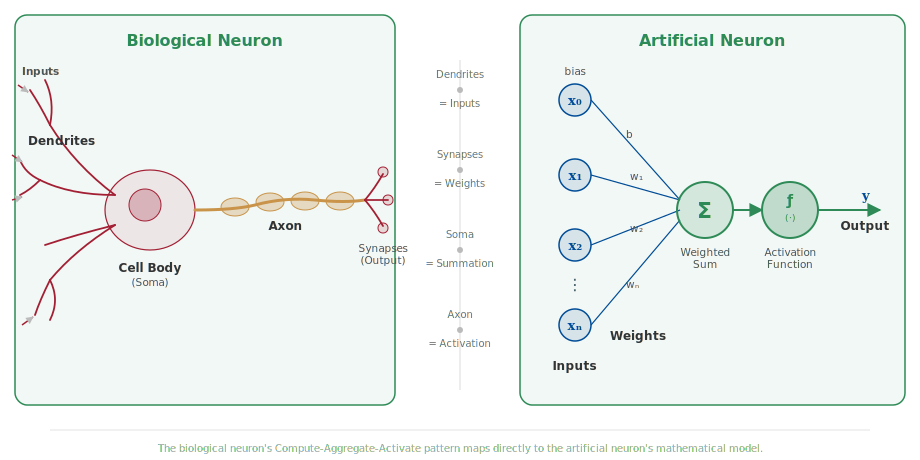
\includegraphics[keepaspectratio]{contents/vol1/dl_primer/images/png/bio_nn2ai_nn.png}}

}

\caption{\label{fig-bio_nn2ai_nn}\textbf{Biological-to-Artificial Neuron
Mapping}: Side-by-side comparison showing how biological neuron
structures map to artificial neuron components. Dendrites correspond to
inputs, synapses to weights, the cell body to the summation function,
and the axon to the activation output. This mapping established the
``Compute-Aggregate-Activate'' pattern central to neural network
design.}

\end{figure}%

Table~\ref{tbl-neuron_structure} formalizes these structural components,
mapping the mathematical functions to their role in the overall
processing pipeline.

\begin{longtable}[]{@{}
  >{\raggedright\arraybackslash}p{(\linewidth - 4\tabcolsep) * \real{0.2376}}
  >{\raggedright\arraybackslash}p{(\linewidth - 4\tabcolsep) * \real{0.3168}}
  >{\raggedright\arraybackslash}p{(\linewidth - 4\tabcolsep) * \real{0.4455}}@{}}
\caption{\textbf{Neuron Structure and Function}: The artificial neuron
functions as a processing pipeline where inputs are modulated by
learnable weights, aggregated into a single signal, and transformed
through a nonlinear activation function. This abstraction enables the
construction of massive networks capable of sophisticated pattern
recognition.}\label{tbl-neuron_structure}\tabularnewline
\toprule\noalign{}
\begin{minipage}[b]{\linewidth}\raggedright
\textbf{Functional Component}
\end{minipage} & \begin{minipage}[b]{\linewidth}\raggedright
\textbf{Mathematical Operation}
\end{minipage} & \begin{minipage}[b]{\linewidth}\raggedright
\textbf{Engineering Role}
\end{minipage} \\
\midrule\noalign{}
\endfirsthead
\toprule\noalign{}
\begin{minipage}[b]{\linewidth}\raggedright
\textbf{Functional Component}
\end{minipage} & \begin{minipage}[b]{\linewidth}\raggedright
\textbf{Mathematical Operation}
\end{minipage} & \begin{minipage}[b]{\linewidth}\raggedright
\textbf{Engineering Role}
\end{minipage} \\
\midrule\noalign{}
\endhead
\bottomrule\noalign{}
\endlastfoot
\textbf{Input Vector} & \(\mathbf{x} = [x_1, \dots, x_n]\) & Data
ingestion from sensors or prior layers \\
\textbf{Weight Vector} & \(\mathbf{w} = [w_1, \dots, w_n]\) & Learnable
parameters encoding importance \\
\textbf{Aggregation} & \(z = \sum (x_i \cdot w_i) + b\) & Linear
integration of feature signals \\
\textbf{Activation} & \(a = \sigma(z)\) & Nonlinear thresholding and
signal propagation \\
\end{longtable}

The processing pipeline operates as follows:

\begin{enumerate}
\def\labelenumi{\arabic{enumi}.}
\item
  \textbf{Input Reception}: The neuron receives a vector of input
  features \(\mathbf{x}\). In a system like MNIST digit recognition,
  these represent individual pixel intensities.
\item
  \textbf{Weighted Modulation}: Each input is multiplied by a learnable
  weight \(w_i\). These weights act as ``gain'' controls, determining
  how much influence each feature has on the final decision. This is
  where the model's ``knowledge'' is stored.
\item
  \textbf{Signal Aggregation (Net Input)}: The neuron integrates the
  weighted signals and adds a bias term \(b\). This produces a single
  scalar value \(z\) representing the evidence for a particular pattern.
\item
  \textbf{Nonlinear Activation}: The aggregated signal passes through an
  activation function \(\sigma(z)\). This nonlinearity is critical: it
  allows the network to model complex, non-linear relationships and acts
  as a threshold, determining whether the neuron ``fires'' a signal to
  the next layer.
\end{enumerate}

From a systems engineering perspective, this translation reveals
\emph{why} neural networks have such demanding computational
requirements. Each ``simple'' neuron requires \(N\) multiply-accumulate
(MAC) operations and \(N+1\) memory accesses. When replicated millions
of times across a network, these primitives create the massive
arithmetic and bandwidth demands that define modern AI infrastructure.

\textbf{Artificial Neural Network Design Principles.} The transition
from individual neurons to integrated systems requires navigating the
fundamental trade-off between representational capacity and
computational cost. While silicon transistors operate at gigahertz
frequencies, millions of times faster than biological chemical
signaling, the sheer volume of operations in deep networks creates
unique bottlenecks.

Replicating intelligent behavior in silicon requires navigating three
system-level constraints:

\begin{itemize}
\tightlist
\item
  \textbf{The Memory Wall}: Neural networks store information in
  discrete weights. As models grow to billions of parameters, moving
  these weights from storage to processing units becomes the primary
  energy and latency bottleneck.
\item
  \textbf{Concurrency vs.~Dependency}: While layers can be computed in
  parallel across thousands of cores (throughput), the sequential nature
  of deep networks (layer \(L+1\) depends on layer \(L\)) creates
  fundamental latency limits.
\item
  \textbf{Precision and Power}: Digital systems achieve high accuracy
  through precise 32-bit or 64-bit math, but each bit increases the
  energy cost of every operation. The drive toward efficiency
  (\textbf{?@sec-model-compression}) involves finding the minimum
  precision required to maintain accuracy while maximizing throughput.
\end{itemize}

Implementing these principles requires two approaches. The first focuses
on \textbf{Architectural Inductive Bias}, designing network structures
(like CNNs for images) that encode problem-specific constraints to
improve efficiency. The second focuses on \textbf{Computational
Scaling}, leveraging massive hardware arrays to solve problems through
brute-force optimization. Modern AI engineering increasingly sits at the
intersection of these two paths: using clever architectures to reduce
the search space and massive scale to find the optimal solution within
it.

\subsection{Mathematical Translation of Neural
Concepts}\label{sec-deep-learning-systems-foundations-mathematical-translation-neural-concepts-8234}

The power of neural networks emerges from their ability to translate
abstract patterns into concrete matrix operations. By organizing neurons
into layers, we can express the entire computation as a series of linear
algebra primitives, which are highly optimized for modern hardware.

Table~\ref{tbl-comp_mapping} maps the conceptual components of the
system to their mathematical and computational implementations.

\begin{longtable}[]{@{}ll@{}}
\caption{\textbf{Conceptual to Computational Mapping}: Deep learning
systems abstract pattern recognition into a series of matrix operations
and nonlinear transformations. This mapping enables efficient digital
implementation while preserving the system's ability to learn complex
hierarchical features.}\label{tbl-comp_mapping}\tabularnewline
\toprule\noalign{}
\textbf{System Component} & \textbf{Computational Implementation} \\
\midrule\noalign{}
\endfirsthead
\toprule\noalign{}
\textbf{System Component} & \textbf{Computational Implementation} \\
\midrule\noalign{}
\endhead
\bottomrule\noalign{}
\endlastfoot
\textbf{Feature Extraction} & Weighted Linear Sum \\
\textbf{Thresholding} & Nonlinear Activation Function \\
\textbf{Pattern Interaction} & Fully-Connected Layer \\
\textbf{Model Memory} & Weight Matrices \& Parameters \\
\textbf{Information Flow} & Forward Propagation \\
\end{longtable}

This mathematical abstraction preserves the essential properties of
learning systems while enabling efficient silicon implementation.
However, this implementation has a physical cost: what appears as a
single matrix multiplication in code translates to millions of
transistors switching at high frequency, generating heat and consuming
significant power. In modern systems, energy efficiency is no longer an
afterthought but a primary design constraint. Large language models can
consume megawatts during training---a scale of energy consumption that
motivates the sustainable engineering practices we explore throughout
this text.

The distributed nature of neural memory also presents a challenge.
Unlike traditional databases where information is stored at specific
addresses, neural ``memory'' is distributed across the entire set of
weights. This means that every prediction requires reading a significant
portion of the model's parameters, placing enormous demands on memory
bandwidth. This ``Memory Wall'' is why modern AI accelerators
(\textbf{?@sec-ai-acceleration}) prioritize high-bandwidth memory (HBM)
over raw processing speed.

\subsection{Hardware and Software
Requirements}\label{sec-deep-learning-systems-foundations-hardware-software-requirements-e1e6}

The computational translation of neural principles creates
infrastructure demands that emerge from key differences between
biological and artificial implementations, directly shaping system
design. Table~\ref{tbl-comp2sys} quantifies how each computational
element drives particular system requirements: activation functions
demand fast nonlinear operation units, weight operations require
high-bandwidth memory access, and learning algorithms necessitate
gradient computation hardware.

\begin{longtable}[]{@{}ll@{}}
\caption{\textbf{Computational Demands}: Artificial neural network
design directly translates into specific system requirements; for
example, efficient activation functions necessitate fast nonlinear
operation units and large-scale weight storage demands high-bandwidth
memory access. Understanding this mapping guides hardware and system
architecture choices for effective implementation of artificial
intelligence.}\label{tbl-comp2sys}\tabularnewline
\toprule\noalign{}
\textbf{Computational Element} & \textbf{System Requirements} \\
\midrule\noalign{}
\endfirsthead
\toprule\noalign{}
\textbf{Computational Element} & \textbf{System Requirements} \\
\midrule\noalign{}
\endhead
\bottomrule\noalign{}
\endlastfoot
\textbf{Activation functions} & Fast nonlinear operation units \\
\textbf{Weight operations} & High-bandwidth memory access \\
\textbf{Parallel computation} & Specialized parallel processors \\
\textbf{Weight storage} & Large-scale memory systems \\
\textbf{Learning algorithms} & Gradient computation hardware \\
\end{longtable}

Storage architecture represents a critical requirement, driven by the
key difference in how biological and artificial systems handle memory.
In biological systems, memory and processing are intrinsically
integrated---synapses both store connection strengths and process
signals. Artificial systems, however, must maintain a clear separation
between processing units and memory. This creates a need for both
high-capacity storage to hold millions or billions of connection weights
and high-bandwidth pathways to move this data quickly between storage
and processing units. The efficiency of this data movement often becomes
a critical bottleneck that biological systems do not face.

The learning process itself imposes distinct requirements on artificial
systems. While biological networks modify synaptic strengths through
local chemical processes, artificial networks must coordinate weight
updates across the entire network. This creates computational and memory
demands during training, as systems must not only store current weights
but also maintain space for gradients and intermediate calculations. The
requirement to backpropagate error signals, with no real biological
analog, complicates the system architecture. Securing these large models
and protecting sensitive training data introduces complex robustness and
security requirements.

Energy efficiency emerges as a final critical requirement, highlighting
perhaps the clearest contrast between biological and artificial
implementations. The human brain operates on approximately 20 watts,
whereas artificial neural networks demand substantially more power.
Current systems often require orders of magnitude more energy to
implement similar capabilities. This gap drives ongoing research in more
efficient hardware architectures and has profound implications for the
practical deployment of neural networks, particularly in
resource-constrained environments like mobile devices or edge computing
systems. The environmental impact of this energy consumption makes
sustainable AI development an increasingly important consideration for
ML systems engineers.

These system requirements directly drive the architectural choices we
make in building ML systems, from the specialized hardware accelerators
covered in \textbf{?@sec-ai-acceleration} to the distributed training
systems discussed in \textbf{?@sec-ai-training}. Understanding why these
requirements exist, rooted in the key differences between biological and
artificial computation, is essential for making informed decisions about
system design and optimization.

\subsection{Evolution of Neural Network
Computing}\label{sec-deep-learning-systems-foundations-evolution-neural-network-computing-8754}

Deep learning evolved to meet these challenges through concurrent
advances in hardware and algorithms. The journey began with early
artificial neural networks in the 1950s, marked by the introduction of
the \textbf{Perceptron}
(\citeproc{ref-rosenblatt1958perceptron}{Rosenblatt
1958})\sidenote{\textbf{Perceptron}: Invented by Frank Rosenblatt in
1957 at Cornell, the perceptron was the first artificial neural network
capable of learning. The New York Times famously reported it would be
``the embryo of an electronic computer that {[}the Navy{]} expects will
be able to walk, talk, see, write, reproduce itself and be conscious of
its existence.'' While overly optimistic, this breakthrough laid the
foundation for all modern neural networks. }. While groundbreaking in
concept, these early systems were severely limited by the computational
capabilities of their era: mainframe computers that lacked both the
processing power and memory capacity needed for complex networks.

The \textbf{backpropagation} algorithm, first applied to neural networks
by Paul Werbos in his 1974 PhD thesis and building on Seppo Linnainmaa's
1970 work on automatic differentiation, was popularized by Rumelhart,
Hinton, and Williams in 1986
(\citeproc{ref-rumelhart1986learning}{Rumelhart, Hinton, and Williams
1986})\sidenote{\textbf{Backpropagation}: Short for ``backward
propagation of errors,'' the name describes how error signals flow
backward through network layers to update weights. The algorithm solves
the ``credit assignment problem'' (determining which weights caused
errors) using the mathematical chain rule. Werbos first applied it to
neural networks in his 1974 PhD thesis
(\citeproc{ref-werbos1974beyond}{Werbos 1974}), building on Linnainmaa's
1970 automatic differentiation work. The 1986 publication by Rumelhart,
Hinton, and Williams (\citeproc{ref-rumelhart1986learning}{Rumelhart,
Hinton, and Williams 1986}) demonstrated practical effectiveness,
triggering the modern deep learning era. }. Their publication
demonstrated the algorithm's practical effectiveness and brought it to
widespread attention in the machine learning community, triggering
renewed interest in neural networks. The systems-level implementation of
this algorithm is detailed in \textbf{?@sec-ai-training}. Despite this
breakthrough, the computational demands far exceeded available hardware
capabilities. Training even modest networks could take weeks, making
experimentation and practical applications challenging. This mismatch
between algorithmic requirements and hardware capabilities contributed
to a period of reduced interest in neural networks.

This historical trajectory offers an important lesson in systems
engineering: a groundbreaking algorithm is only as powerful as the
hardware available to execute it. The decades-long gap between the
mathematical formulation of backpropagation and its widespread adoption
was not a failure of theory, but a latency in infrastructure. It teaches
us that efficient ML systems engineering is not just about designing for
the best math, but co-designing for the available silicon. The eventual
deep learning revolution was sparked not by a new mathematical discovery
alone, but by the convergence of data availability, algorithmic
maturity, and the parallel processing power of GPUs.

While the preceding sections established the technical foundations of
deep learning, the term itself gained prominence in the 2010s,
coinciding with advances in computational power and data accessibility.
Two remarkable trends emerge from Figure~\ref{fig-trends}: computational
capabilities measured in floating-point operations per second (FLOPS)
initially followed a \(1.4\times\) improvement pattern from 1952 to
2010, then accelerated to a 3.4-month doubling cycle from 2012 to 2022.
The emergence of large-scale models between 2015 and 2022 (not
explicitly shown or easily seen in Figure~\ref{fig-trends}) is perhaps
more striking still: these scaled 2 to 3 orders of magnitude faster than
the general trend, following an aggressive 10-month doubling cycle.

\begin{figure}[htb]

\centering{

\pandocbounded{\includegraphics[keepaspectratio]{contents/vol1/dl_primer/images/png/trends_65d82031.png}}

}

\caption{\label{fig-trends}\textbf{Computational Growth}: Log-scale
scatter plot showing training compute in FLOPS from 1952 to 2022.
Computational power grew at a 1.4x rate from 1952 to 2010, then
accelerated to a doubling every 3.4 months from 2012 to 2022.
Large-scale models after 2015 followed an even faster 10-month doubling
cycle, addressing the historical bottleneck of training complex neural
networks.}

\end{figure}%

Table~\ref{tbl-historical-performance} grounds these trends in concrete
systems, showing how parameters, compute, and hardware co-evolved across
four decades of neural network development.

\begin{longtable}[]{@{}
  >{\raggedright\arraybackslash}p{(\linewidth - 12\tabcolsep) * \real{0.0734}}
  >{\raggedright\arraybackslash}p{(\linewidth - 12\tabcolsep) * \real{0.0917}}
  >{\raggedleft\arraybackslash}p{(\linewidth - 12\tabcolsep) * \real{0.1560}}
  >{\raggedleft\arraybackslash}p{(\linewidth - 12\tabcolsep) * \real{0.1743}}
  >{\raggedleft\arraybackslash}p{(\linewidth - 12\tabcolsep) * \real{0.2294}}
  >{\raggedright\arraybackslash}p{(\linewidth - 12\tabcolsep) * \real{0.1284}}
  >{\raggedright\arraybackslash}p{(\linewidth - 12\tabcolsep) * \real{0.1468}}@{}}
\caption{\textbf{Historical Performance}: Four decades of neural network
evolution showing the co-scaling of model parameters, training compute,
and hardware infrastructure. Training FLOPs increased by approximately
\(10^{13}\)× from LeNet-1 to GPT-4, while parameters grew by
\(10^{8}\)×. \textbf{Uncertainty notes}: Earlier systems (LeNet,
AlexNet) have well-documented specifications; recent closed models
(GPT-4) have only external estimates. ``OoM'' = order of magnitude
uncertainty.}\label{tbl-historical-performance}\tabularnewline
\toprule\noalign{}
\begin{minipage}[b]{\linewidth}\raggedright
\textbf{Year}
\end{minipage} & \begin{minipage}[b]{\linewidth}\raggedright
\textbf{System}
\end{minipage} & \begin{minipage}[b]{\linewidth}\raggedleft
\textbf{Params}
\end{minipage} & \begin{minipage}[b]{\linewidth}\raggedleft
\textbf{Train FLOPs}
\end{minipage} & \begin{minipage}[b]{\linewidth}\raggedleft
\textbf{Hardware}
\end{minipage} & \begin{minipage}[b]{\linewidth}\raggedright
\textbf{Train Time}
\end{minipage} & \begin{minipage}[b]{\linewidth}\raggedright
\textbf{Error/Task}
\end{minipage} \\
\midrule\noalign{}
\endfirsthead
\toprule\noalign{}
\begin{minipage}[b]{\linewidth}\raggedright
\textbf{Year}
\end{minipage} & \begin{minipage}[b]{\linewidth}\raggedright
\textbf{System}
\end{minipage} & \begin{minipage}[b]{\linewidth}\raggedleft
\textbf{Params}
\end{minipage} & \begin{minipage}[b]{\linewidth}\raggedleft
\textbf{Train FLOPs}
\end{minipage} & \begin{minipage}[b]{\linewidth}\raggedleft
\textbf{Hardware}
\end{minipage} & \begin{minipage}[b]{\linewidth}\raggedright
\textbf{Train Time}
\end{minipage} & \begin{minipage}[b]{\linewidth}\raggedright
\textbf{Error/Task}
\end{minipage} \\
\midrule\noalign{}
\endhead
\bottomrule\noalign{}
\endlastfoot
1989 & LeNet-1 & \textasciitilde9.8K & \(10^{11}\)--\(10^{12}\) &
Sun-4/260 workstation & 3 days & 1.0\% (USPS) \\
1998 & LeNet-5 & 60K ±1K & \(10^{14}\) ±1 OoM & SGI Origin 2000 (200
MHz) & 2-3 days & 0.95\% (MNIST) \\
2012 & AlexNet & \textasciitilde60M & \(5 \times 10^{17}\) & 2× GTX 580
GPUs & 5-6 days & 15.3\% (ImageNet) \\
2015 & ResNet-152 & \textasciitilde60M & \(10^{19}\) ±0.5 OoM & 8× Tesla
K80 GPUs & \textasciitilde3 weeks & 3.6\% (ImageNet) \\
2020 & GPT-3 & 175B (exact) & \(3 \times 10^{23}\) & \textasciitilde10K
V100 GPUs & weeks & N/A (language) \\
2023 & GPT-4 & \textasciitilde1.8T (MoE, est.) &
\(10^{24}\)--\(10^{25}\) & 10-25K A100s (est.) & months & N/A
(language) \\
\end{longtable}

Beyond raw compute, this exponential growth has profound environmental
implications. Consider the energy costs behind these scaling trends,
which reveal what we call \emph{the carbon footprint of AI evolution}.

\phantomsection\label{callout-notebookux2a-1.3}
\begin{fbxSimple}{callout-notebook}{AI Engineer’s Notebook:}{The Carbon Footprint of AI Evolution}
\phantomsection\label{callout-notebook*-1.3}
\textbf{The Energy Scale Factor}: As we scale from LeNet to GPT-4, we
are not just scaling parameters; we are scaling computational
requirements by 13 orders of magnitude.

\begin{enumerate}
\def\labelenumi{\arabic{enumi}.}
\tightlist
\item
  \textbf{LeNet-1 (1989)}: Training took days on a workstation consuming
  \textasciitilde200W. Total Energy \(\approx\) \textbf{50 kWh}.
\item
  \textbf{ResNet-50 (2015)}: Training takes weeks on 8 GPUs. Total
  Energy \(\approx\) \textbf{10 MWh}.
\item
  \textbf{GPT-4 (2023)}: Training takes months on \textasciitilde25,000
  GPUs. Total Energy \(\approx\) \textbf{50,000 MWh}.
\end{enumerate}

\textbf{The Systems Conclusion}: The energy cost of AI has moved from
``negligible'' (a lightbulb) to ``industrial'' (a city). This shift
forces systems engineers to treat \textbf{Energy Efficiency} (Joules/Op)
as a primary design constraint, equal to or greater than FLOPS. The
\textbf{Energy Corollary} to the Iron Law is not theoretical; it is an
economic and environmental imperative.

\end{fbxSimple}

Three quantitative ``laws'' emerge from this historical data that inform
modern systems engineering:

\begin{enumerate}
\def\labelenumi{\arabic{enumi}.}
\item
  \textbf{The Compute Scaling Law}: Training compute for frontier AI
  models grows approximately \textbf{4-5× per year}, with a doubling
  time of \textasciitilde5-6 months---roughly 4× faster than Moore's Law
  for transistor density.
\item
  \textbf{The Algorithmic Efficiency Law}: The compute required to
  achieve a fixed benchmark performance halves approximately every
  \textbf{8 months for language models} (5-14 months 95\% CI) due to
  algorithmic improvements (better architectures, optimizers, training
  techniques), separate from and faster than hardware gains alone. For
  image classification, the doubling time is approximately 16 months.
\item
  \textbf{The Cost-Compute Gap}: While compute grows \textasciitilde4-5×
  per year, training \emph{costs} grow only \textasciitilde2.4× per
  year, reflecting efficiency gains in hardware utilization, reduced
  precision arithmetic, and scale economies. Nevertheless, frontier
  model training costs have risen from thousands of dollars (LeNet era)
  to over \$100 million (GPT-4 era).
\end{enumerate}

These laws have direct implications for systems engineering: the compute
scaling law determines infrastructure investment timelines, the
algorithmic efficiency law justifies continuous architecture research,
and the cost-compute gap shapes build-versus-buy decisions for ML teams.

\phantomsection\label{callout-perspectiveux2a-1.4}
\begin{fbxSimple}{callout-perspective}{Systems Perspective:}{The Energy Cost of Intelligence}
\phantomsection\label{callout-perspective*-1.4}

Beyond dollar costs, neural network computation consumes substantial
energy, a consideration increasingly important for sustainable AI
development and edge deployment where power budgets are constrained.
Table~\ref{tbl-energy-costs} summarizes energy consumption across neural
network scales.

\begin{longtable}[]{@{}
  >{\raggedright\arraybackslash}p{(\linewidth - 6\tabcolsep) * \real{0.2436}}
  >{\raggedleft\arraybackslash}p{(\linewidth - 6\tabcolsep) * \real{0.2564}}
  >{\raggedleft\arraybackslash}p{(\linewidth - 6\tabcolsep) * \real{0.2692}}
  >{\raggedleft\arraybackslash}p{(\linewidth - 6\tabcolsep) * \real{0.2308}}@{}}
\caption{\textbf{Energy Consumption Across Neural Network Scales}: CO₂
estimates assume US average grid (\textasciitilde0.5 kg CO₂/kWh).
Inference energy assumes single request; training energy covers full
model development. *BERT-base figure includes hyperparameter tuning;
base training alone is lower.}\label{tbl-energy-costs}\tabularnewline
\toprule\noalign{}
\begin{minipage}[b]{\linewidth}\raggedright
\textbf{System}
\end{minipage} & \begin{minipage}[b]{\linewidth}\raggedleft
\textbf{Energy/Inference}
\end{minipage} & \begin{minipage}[b]{\linewidth}\raggedleft
\textbf{Energy/Training}
\end{minipage} & \begin{minipage}[b]{\linewidth}\raggedleft
\textbf{CO₂ Equivalent}
\end{minipage} \\
\midrule\noalign{}
\endfirsthead
\toprule\noalign{}
\begin{minipage}[b]{\linewidth}\raggedright
\textbf{System}
\end{minipage} & \begin{minipage}[b]{\linewidth}\raggedleft
\textbf{Energy/Inference}
\end{minipage} & \begin{minipage}[b]{\linewidth}\raggedleft
\textbf{Energy/Training}
\end{minipage} & \begin{minipage}[b]{\linewidth}\raggedleft
\textbf{CO₂ Equivalent}
\end{minipage} \\
\midrule\noalign{}
\endhead
\bottomrule\noalign{}
\endlastfoot
\textbf{MNIST MLP (CPU)} & \textasciitilde0.1 mJ & \textasciitilde10 J
(full training) & \textasciitilde0.005 g \\
\textbf{MNIST MLP (GPU)} & \textasciitilde0.01 mJ & \textasciitilde1 J &
\textasciitilde0.0005 g \\
\textbf{ResNet-50} & \textasciitilde10 mJ & \textasciitilde100 kWh &
\textasciitilde50 kg \\
\textbf{BERT-base} & \textasciitilde50 mJ & \textasciitilde1,500 kWh* &
\textasciitilde635 kg \\
\textbf{GPT-3} & \textasciitilde1 J & \textasciitilde1,287 MWh &
\textasciitilde552 tonnes \\
\textbf{GPT-4 (est.)} & \textasciitilde10 J & \textasciitilde50,000 MWh
& \textasciitilde25,000 tonnes \\
\end{longtable}

\textbf{Key insights for systems engineers:}

\begin{enumerate}
\def\labelenumi{\arabic{enumi}.}
\tightlist
\item
  \textbf{Data movement dominates}: Moving a byte from DRAM costs
  \textasciitilde100× more energy than a floating-point operation.
  Optimizing data locality matters more than raw compute speed for
  energy efficiency.
\item
  \textbf{Inference vs Training}: Training GPT-3 consumed energy
  equivalent to \textasciitilde120 US households for a year---but each
  inference consumes only \textasciitilde1 J. At scale, inference energy
  often exceeds training energy (GPT-3 serves billions of queries).
\item
  \textbf{Edge deployment constraint}: Mobile devices budget 1-5W for ML
  inference. A 10 mJ/inference model can run at 100-500
  inferences/second within this budget; a 1 J/inference model is
  impractical for real-time mobile use.
\item
  \textbf{The efficiency imperative}: Energy costs provide strong
  economic incentive for model compression
  (\textbf{?@sec-model-compression}) and efficient architectures
  (\textbf{?@sec-dnn-architectures}). A 10× energy reduction translates
  directly to 10× cost reduction at scale.
\end{enumerate}

\end{fbxSimple}

The dominance of data movement in energy consumption has profound
implications for architecture design. The following engineering
calculation reveals \emph{the physics of efficiency} at the transistor
level.

\phantomsection\label{callout-notebookux2a-1.5}
\begin{fbxSimple}{callout-notebook}{AI Engineer’s Notebook:}{The Physics of Efficiency}
\phantomsection\label{callout-notebook*-1.5}
\textbf{Why Data Movement Dominates:} To understand why architectures
like CNNs (high reuse) are more efficient than MLPs (low reuse), we must
look at the energy cost of operations at the transistor level.

\begin{longtable}[]{@{}
  >{\raggedright\arraybackslash}p{(\linewidth - 4\tabcolsep) * \real{0.2553}}
  >{\raggedright\arraybackslash}p{(\linewidth - 4\tabcolsep) * \real{0.3085}}
  >{\raggedright\arraybackslash}p{(\linewidth - 4\tabcolsep) * \real{0.4362}}@{}}
\toprule\noalign{}
\begin{minipage}[b]{\linewidth}\raggedright
\textbf{Operation (45nm)}
\end{minipage} & \begin{minipage}[b]{\linewidth}\raggedright
\textbf{Energy (pJ)}
\end{minipage} & \begin{minipage}[b]{\linewidth}\raggedright
\textbf{Relative Cost}
\end{minipage} \\
\midrule\noalign{}
\endhead
\bottomrule\noalign{}
\endlastfoot
\textbf{FP32 Add} & 0.9 pJ & 1\(\times\) \\
\textbf{FP32 Multiply} & 3.7 pJ & 4\(\times\) \\
\textbf{SRAM Access (32-bit)} & 5.0 pJ & 5\(\times\) \\
\textbf{DRAM Access (32-bit)} & \textbf{640.0 pJ} &
\textbf{711\(\times\)} \\
\end{longtable}

\emph{Source: Mark Horowitz, ``Computing's Energy Problem'' (ISSCC
2014).}

\textbf{The Engineering Implication:} Fetching a weight from DRAM costs
\textbf{711 times more energy} than multiplying it.

\begin{itemize}
\tightlist
\item
  \textbf{Inefficient:} Read weight \(\to\) Multiply \(\to\) Write. Cost
  \(\approx 1284\) pJ.
\item
  \textbf{Efficient:} Read weight \(\to\) Multiply 100 times (Reuse)
  \(\to\) Write. Cost per op drops dramatically.
\end{itemize}

This physics dictates why \textbf{Arithmetic Intensity} (Ops/Byte) is
the fundamental metric of efficient computing.

\end{fbxSimple}

Parallel advances across three dimensions drove these evolutionary
trends: data availability, algorithmic innovations, and computing
infrastructure. Figure~\ref{fig-virtuous-cycle} captures this
reinforcing cycle: more powerful computing infrastructure enabled
processing larger datasets, larger datasets drove algorithmic
innovations, and better algorithms demanded more sophisticated computing
systems. This reinforcing cycle continues to drive progress today.

\begin{figure}[htb]

\centering{

\pandocbounded{\includegraphics[keepaspectratio]{index_files/mediabag/5832d666949320d0ce8c30b98230f4afbb26a195.pdf}}

}

\caption{\label{fig-virtuous-cycle}\textbf{Deep Learning Virtuous
Cycle}: Three mutually reinforcing factors, data availability,
algorithmic innovations, and computing infrastructure, form a
self-reinforcing loop where breakthroughs in one area create
opportunities in the others.}

\end{figure}%

The data revolution transformed what was possible with neural networks.
The rise of the internet and digital devices created vast new sources of
training data: image sharing platforms provided millions of labeled
images, digital text collections enabled language processing at scale,
and sensor networks generated continuous streams of real-world data.
This abundance provided the raw material neural networks needed to learn
complex patterns effectively.

Algorithmic innovations made it possible to use this data effectively.
New methods for initializing networks and controlling learning rates
made training more stable. Techniques for preventing
overfitting\sidenote{\textbf{Overfitting}: The term emerged from
statistics, where ``fitting'' describes how well a model matches data.
``Over-fitting'' occurs when a model matches training data too
precisely, capturing noise rather than underlying patterns. The concept
dates to early 20th-century statistics, but became central to ML through
the bias-variance tradeoff framework. Occam's Razor (14th century)
anticipated this idea: simpler explanations that fit the data are
preferable to complex ones that fit perfectly but fail to generalize. }
allowed models to generalize better to new data. Researchers discovered
that neural network performance scaled predictably with model size,
computation, and data quantity, leading to increasingly ambitious
architectures.

These algorithmic advances created demand for more powerful computing
infrastructure, which evolved in response. On the hardware side, GPUs
provided the parallel processing capabilities needed for efficient
neural network computation, and specialized AI accelerators like
TPUs\sidenote{\textbf{Tensor Processing Unit (TPU)}: Google's custom
silicon designed specifically for tensor operations, the mathematical
building blocks of neural networks. First deployed internally in 2015,
TPUs can perform matrix multiplications up to 30× faster than 2015-era
GPUs while using less power. The name reflects their optimization for
tensor operations---multi-dimensional arrays that represent data flowing
through neural networks. Google has since made TPUs available through
cloud services, democratizing access to this specialized AI hardware. }
(\citeproc{ref-jouppi2023tpu}{Jouppi et al. 2023}) pushed performance
further. High-bandwidth memory systems and fast interconnects addressed
data movement challenges. Equally important were software advances:
frameworks and libraries\sidenote{\textbf{Deep Learning Frameworks}:
Software libraries like TensorFlow and PyTorch that provide high-level
abstractions for building and training neural networks. Framework design
and selection are detailed in \textbf{?@sec-ai-frameworks}. } that
simplified building and training networks, distributed computing systems
that enabled training at scale, and tools for optimizing model
deployment.

The convergence of data availability, algorithmic innovation, and
computational infrastructure created the foundation for modern deep
learning. Building effective ML systems requires understanding the
computational operations that drive these infrastructure requirements,
because when scaled across millions of parameters and billions of
training examples, simple mathematical operations create the massive
computational demands that shaped this evolution.

\phantomsection\label{callout-checkpointux2a-1.6}
\begin{fbxSimple}{callout-checkpoint}{Checkpoint:}{Understanding Deep Learning's Emergence}
\phantomsection\label{callout-checkpoint*-1.6}
Before proceeding to the mathematical foundations, verify your
understanding of why deep learning emerged:

\begin{itemize}
\tightlist
\item[$\square$]
  Can you explain why rule-based programming fails for tasks like image
  recognition?
\item[$\square$]
  Do you understand the difference between classical ML (feature
  engineering) and deep learning (automatic feature learning)?
\item[$\square$]
  Can you describe the three factors that converged to enable modern
  deep learning (data, algorithms, infrastructure)?
\item[$\square$]
  Do you understand why deep learning requires specialized hardware
  compared to traditional programming?
\end{itemize}

If any of these concepts remain unclear, review the relevant sections
before continuing. The mathematical details that follow build directly
on this conceptual foundation.

\end{fbxSimple}

Having established why deep learning emerged and what infrastructure it
requires, we now examine the mathematical building blocks that create
these computational demands.

\section{Neural Network
Fundamentals}\label{sec-deep-learning-systems-foundations-neural-network-fundamentals-07e4}

The infrastructure demands we examined (massive parallelism, high memory
bandwidth, specialized accelerators) arise directly from the
mathematical operations neural networks perform. To understand
\emph{why} a GPU processes neural networks faster than a CPU, or
\emph{why} training requires more memory than inference, we must examine
the operations themselves. This section develops that mathematical
foundation, showing how simple operations on individual neurons compound
into the computational requirements that shaped modern AI
infrastructure.

The concepts here apply to all neural networks, from simple classifiers
to large language models. While architectures evolve and new paradigms
emerge, these fundamentals remain constant: weighted sums, nonlinear
activations, gradient-based learning. Master these operations and their
computational characteristics, and you can reason about any neural
network's resource requirements.

\subsection{Why Depth Matters: The Power of Hierarchical
Representations}\label{sec-deep-learning-systems-foundations-depth-matters-power-hierarchical-representations-f83c}

Before examining the mathematical machinery of neural networks, we
preview why ``deep'' learning earns its name. The detailed mechanics of
layers and connections follow in subsequent sections; here we establish
the intuition for why depth provides such dramatic representational
advantages. We introduced hierarchical feature learning conceptually
when discussing the evolution from classical machine learning; now we
formalize that intuition with a concrete example that grounds all
subsequent mathematical development.

Deep networks succeed because they leverage \textbf{compositionality}:
complex patterns decompose into simpler patterns that themselves
decompose further. In image recognition, pixels combine into edges,
edges into textures, textures into parts, and parts into objects. This
hierarchical decomposition reflects the structure of the world itself
and explains why ``deep'' learning earns its name.

Consider recognizing the digit ``7'' in our MNIST example. A
single-layer network would need to directly map all 784 pixel values to
a decision, essentially memorizing every variation of how people write
``7.'' A deep network takes a fundamentally different approach:

\begin{itemize}
\tightlist
\item
  \textbf{Layer 1} learns simple edge detectors---vertical lines,
  horizontal lines, diagonal strokes
\item
  \textbf{Layer 2} combines edges into shapes---the horizontal top
  stroke of a ``7,'' the diagonal downstroke
\item
  \textbf{Layer 3} combines shapes into complete digit patterns
\end{itemize}

Each layer builds on the previous, exponentially expanding
representational capacity with only linear parameter growth. This
hierarchy enables efficiency that shallow networks cannot match. The
same edge detectors learned for ``7'' also detect edges in ``1,'' ``4,''
and every other digit. This \textbf{parameter reuse} means a deep
network with 100K parameters can represent patterns that would require
millions of parameters in a shallow network attempting direct
pixel-to-label mapping. However, the choice between adding layers and
widening existing ones involves a fundamental \emph{depth vs.~width
tradeoff}.

\phantomsection\label{callout-perspectiveux2a-1.7}
\begin{fbxSimple}{callout-perspective}{Systems Perspective:}{The Depth vs. Width Tradeoff}
\phantomsection\label{callout-perspective*-1.7}
The theoretical power of depth comes from the \textbf{exponential
advantage}: a network with \(L\) layers can represent functions that
require exponentially more (\(2^L\)) neurons in a single-layer network.
This follows from the fact that each layer doubles the complexity of
decision boundaries it can express.

However, depth introduces engineering challenges. Each additional layer:

\begin{itemize}
\tightlist
\item
  Adds sequential dependencies (layer \(L+1\) waits for layer \(L\)),
  limiting parallelism
\item
  Increases gradient path length, risking vanishing/exploding gradients
\item
  Requires storing intermediate activations for backpropagation
\end{itemize}

Modern architectures balance depth (representational power) against
width (parallelism). A network with 10 layers of 100 neurons has the
same 1,000 neurons per input as one with 2 layers of 500 neurons, but
very different computational characteristics. The deeper network can
represent more complex functions; the wider network can compute all
neurons in a layer simultaneously.

\end{fbxSimple}

This hierarchical decomposition is a powerful computational strategy,
one that biological visual systems also employ. The specific
architectures examined in \textbf{?@sec-dnn-architectures} formalize
different ways to encode this hierarchical structure, from the local
connectivity of convolutional networks to the attention mechanisms of
transformers.

With the intuition for \emph{why} depth matters established, we now
examine \emph{how} neural networks implement this hierarchical
processing. The following sections develop the precise mechanics: how
neurons compute, how layers connect, and how information flows from
input to output.

\subsection{Network Architecture
Fundamentals}\label{sec-deep-learning-systems-foundations-network-architecture-fundamentals-1f58}

The architecture of a neural network determines how information flows
from input to output. While modern networks can be tremendously complex,
they all build upon a few organizational principles that directly impact
system design. Understanding these principles is necessary for both
implementing neural networks and appreciating why they require the
computational infrastructure discussed above.

To ground these concepts in a concrete example, we use handwritten digit
recognition throughout this section, specifically the task of
classifying images from the MNIST dataset
(\citeproc{ref-lecun1998gradient}{Lecun et al. 1998}). This seemingly
simple task reveals all the fundamental principles of neural networks
while providing intuition for more complex applications.

\phantomsection\label{callout-exampleux2a-1.8}
\begin{fbxSimple}{callout-example}{Example:}{Running Example: MNIST Digit Recognition}
\phantomsection\label{callout-example*-1.8}
\textbf{The Task}: Given a 28×28 pixel grayscale image of a handwritten
digit, classify it as one of the ten digits (0--9).

\textbf{Input Representation}: Each image contains 784 pixels (28×28),
with values ranging from 0 (white) to 255 (black). We normalize these to
the range {[}0,1{]} by dividing by 255. When fed to a neural network,
these 784 values form our input vector
\(\mathbf{x} \in \mathbb{R}^{784}\).

\textbf{Output Representation}: The network produces 10 values, one for
each possible digit. These values represent the network's confidence
that the input image contains each digit. The digit with the highest
confidence becomes the prediction.

\textbf{Why This Example}: MNIST is small enough to understand
completely (784 inputs, \textasciitilde100K parameters for a simple
network) yet large enough to be realistic. The task is intuitive:
everyone understands what ``recognize a handwritten 7'' means, making it
ideal for learning neural network principles that scale to much larger
problems.

\textbf{Network Architecture Preview}: A typical MNIST classifier might
use: 784 input neurons (one per pixel) → 128 hidden neurons → 64 hidden
neurons → 10 output neurons (one per digit class). As we develop
concepts, we'll reference this specific architecture.

\end{fbxSimple}

Each architectural choice, from how neurons are connected to how layers
are organized, creates specific computational patterns that must be
efficiently mapped to hardware. This mapping between network
architecture and computational requirements is essential for building
scalable ML systems.

\subsubsection{Nonlinear Activation
Functions}\label{sec-deep-learning-systems-foundations-nonlinear-activation-functions-38bc}

With the conceptual framework of layers and hierarchical processing
established, we now examine the computational machinery within each
layer. Central to all neural architectures is a basic building block:
the artificial neuron or perceptron, which implements the
biological-to-artificial translation principles established earlier.
From a systems perspective, understanding the perceptron's mathematical
operations matters because these simple operations, replicated millions
of times across a network, create the computational bottlenecks
discussed above.

Consider our MNIST digit recognition task. Each pixel in a 28x28 image
becomes an input to our network. A single neuron in the first hidden
layer might learn to detect a specific pattern, perhaps a vertical edge
that appears in digits like ``1'' or ``7.'' This neuron must somehow
combine all 784 pixel values into a single output that indicates whether
its pattern is present.

The perceptron accomplishes this through weighted summation. It takes
multiple inputs \(x_1, x_2, ..., x_n\) (in our case, \(n=784\) pixel
values), each representing a feature of the object under analysis. For
digit recognition, these features are simply the raw pixel intensities,
though for other tasks they might be the characteristics of a home for
predicting its price or the attributes of a song to forecast its
popularity.

This multiplication process reveals the computational complexity beneath
apparently simple operations. Each input requires storage in memory and
retrieval during processing. When multiplied across millions of neurons
in a deep network, these memory access patterns become a primary
performance bottleneck, which is why the memory hierarchy and bandwidth
considerations discussed earlier are so critical to neural network
performance.

With this weighted summation, a perceptron can perform either regression
or classification tasks. For regression, the numerical output
\(\hat{y}\) is used directly. For classification, the output depends on
whether \(\hat{y}\) crosses a threshold: above the threshold, the
perceptron outputs one class (e.g., ``yes''); below it, another class
(e.g., ``no'').

Figure~\ref{fig-perceptron} illustrates how weighted inputs combine with
activation functions to enable pattern recognition: each input \(x_i\)
multiplies by its corresponding weight \(w_{ij}\), the products sum with
a bias term, and the activation function produces the final output.

\begin{figure}[htb]

\centering{

\pandocbounded{\includegraphics[keepaspectratio]{index_files/mediabag/306caa56c287a8fa9e0178945b95ad56a11e5a61.pdf}}

}

\caption{\label{fig-perceptron}\textbf{Perceptron Architecture}: The
fundamental computational unit of neural networks, showing inputs
multiplied by weights, summed with bias, and passed through an
activation function to produce output.}

\end{figure}%

Scaling beyond individual units, layers of perceptrons work in concert,
with each layer's output serving as the input for the subsequent layer.
This hierarchical arrangement creates deep learning models capable of
tackling increasingly sophisticated tasks, from image recognition to
natural language processing.

Breaking down the computational mechanics, each input \(x_i\) has a
corresponding weight \(w_{ij}\), and the perceptron simply multiplies
each input by its matching weight. The intermediate output, \(z\), is
computed as the weighted sum of inputs:
\[ z = \sum (x_i \cdot w_{ij}) \]

The apparent simplicity of this expression masks its computational
complexity. Scaled across millions of neurons and billions of
parameters, these memory access patterns become the dominant performance
bottleneck in neural network computation.

To enhance the model's flexibility, a bias term \(b\) is added to this
intermediate calculation, allowing the model to better fit the data by
shifting the linear output function up or down. Thus, the intermediate
linear combination computed by the perceptron including the bias
becomes: \[ z = \sum (x_i \cdot w_{ij}) + b \]

This mathematical formulation directly drives the hardware requirements
we discussed earlier. The summation requires accumulator units, the
multiplications demand high-throughput arithmetic units, and the memory
accesses necessitate high-bandwidth memory systems. Understanding this
connection between mathematical operations and hardware requirements is
crucial for designing efficient ML systems.

Activation functions are critical nonlinear transformations that enable
neural networks to learn complex patterns by converting linear weighted
sums into nonlinear outputs. Without activation functions, multiple
linear layers would collapse into a single linear transformation,
severely limiting the network's expressive power. Four commonly used
activation functions each exhibit distinct mathematical characteristics
that shape their effectiveness in different contexts
(Figure~\ref{fig-activation-functions}).

\begin{figure}[htb]

\centering{

\pandocbounded{\includegraphics[keepaspectratio]{index_files/mediabag/643bc46a41d949aa4c16b0115a33288df2bfb1fc.pdf}}

}

\caption{\label{fig-activation-functions}\textbf{Common Activation
Functions}: Four nonlinear activation functions plotted with their
output ranges. Sigmoid maps inputs to \((0,1)\) with smooth gradients,
tanh provides zero-centered outputs in \((-1,1)\), ReLU introduces
sparsity by outputting zero for negative inputs, and softmax converts
logits into probability distributions.}

\end{figure}%

The choice of activation function affects both learning effectiveness
and computational efficiency. The mathematical properties of each
function shape its suitability for different contexts. The most commonly
used activation functions include:

\paragraph{Sigmoid}\label{sec-deep-learning-systems-foundations-sigmoid-a98f}

The sigmoid function\sidenote{\textbf{Sigmoid}: From the Greek letter
sigma (Σ, σ) combined with ``-oid'' meaning ``resembling.'' The
function's S-shaped curve visually resembles the letter sigma. First
described mathematically by Pierre-Francois Verhulst in 1845 for
modeling population growth, the sigmoid became central to neural
networks because its smooth, bounded output (0 to 1) naturally
represents probabilities. The term ``logistic function'' is often used
interchangeably, from the Greek ``logistikos'' (skilled in calculating).
\[ \sigma(x) = \frac{1}{1 + e^{-x}} \] } maps any input value to a
bounded range between 0 and 1:

This S-shaped curve produces outputs that can be interpreted as
probabilities, making sigmoid particularly useful for binary
classification tasks. For very large positive inputs, the function
approaches 1; for very large negative inputs, it approaches 0. The
smooth, continuous nature of sigmoid makes it differentiable everywhere,
which is necessary for gradient-based learning.

Sigmoid has a significant limitation: for inputs with large absolute
values (far from zero), the gradient becomes extremely small, a
phenomenon called the \textbf{vanishing gradient
problem}\sidenote{\textbf{Vanishing Gradients}: When gradients become
exponentially small as they propagate backward through many layers,
learning effectively stops in early layers
(\citeproc{ref-hochreiter1998vanishing}{Hochreiter 1998}). This occurs
because gradients are computed via the chain rule, multiplying
derivatives from each layer. If these derivatives are consistently less
than 1 (as with saturated sigmoid outputs), their product shrinks
exponentially with network depth. This problem is addressed in detail in
\textbf{?@sec-ai-training}. }. During backpropagation, these small
gradients multiply together across layers, causing gradients in early
layers to become exponentially tiny. This effectively prevents learning
in deep networks, as weight updates become negligible.

Sigmoid outputs are not zero-centered (all outputs are positive). This
asymmetry can cause inefficient weight updates during optimization, as
gradients for weights connected to sigmoid units will all have the same
sign.

\paragraph{Tanh}\label{sec-deep-learning-systems-foundations-tanh-e981}

The hyperbolic tangent function\sidenote{\textbf{Tanh (Hyperbolic
Tangent)}: ``Hyperbolic'' functions were named by Vincenzo Riccati in
1757 because their geometric relationship to hyperbolas mirrors how
circular trigonometric functions relate to circles. The ``tangent''
comes from Latin ``tangens'' (touching), describing a line touching a
curve at one point. While sinh and cosh model hanging chains
(catenaries) in physics, tanh found its role in neural networks because
it maps any input to (-1, 1) with zero-centered outputs, improving
gradient flow compared to sigmoid's (0, 1) range.
\[ \tanh(x) = \frac{e^x - e^{-x}}{e^x + e^{-x}} \] } addresses sigmoid's
zero-centering limitation by mapping inputs to the range \((-1, 1)\):

The tanh function produces an S-shaped curve similar to sigmoid but
centered at zero. Negative inputs map to negative outputs, while
positive inputs map to positive outputs. This symmetry helps balance
gradient flow during training, often leading to faster convergence than
sigmoid.

Like sigmoid, tanh is smooth and differentiable everywhere, and it still
suffers from the vanishing gradient problem for inputs with large
magnitudes. When the function saturates (approaches -1 or 1), gradients
become very small. Despite this limitation, tanh's zero-centered outputs
make it preferable to sigmoid for hidden layers in many architectures,
particularly in recurrent neural networks where maintaining balanced
activations across time steps is important.

Both sigmoid and tanh share a fundamental limitation: gradient
saturation at extreme input values. The search for an activation
function that avoids this problem while remaining computationally
efficient led to one of deep learning's most important innovations.

\paragraph{ReLU}\label{sec-deep-learning-systems-foundations-relu-7184}

The Rectified Linear Unit (ReLU) function was known for decades before
deep learning, but Nair and Hinton demonstrated in 2010 that it enabled
more effective training of deep networks
(\citeproc{ref-nair2010rectified}{Nair and Hinton
2010})\sidenote{\textbf{ReLU (Rectified Linear Unit)}: ``Rectified''
comes from Latin ``rectus'' (straight) and describes the function's
behavior of passing positive values straight through while zeroing
negatives, similar to electrical rectifiers that convert AC to DC by
blocking negative voltage. The mathematical function \(\max(0, x)\) was
known for decades, but Nair and Hinton (2010) demonstrated its
effectiveness for deep networks. ReLU's computational simplicity (one
comparison vs.~exponentials for sigmoid) and constant gradient for
positive values made it the default activation that enabled the deep
learning revolution. }. Combined with GPU computing,
dropout\sidenote{\textbf{Dropout}: A regularization technique introduced
by Srivastava et al. (\citeproc{ref-srivastava2014dropout}{Srivastava et
al. 2014}) that randomly sets a fraction of neuron outputs to zero
during training, typically 20-50\%. This forces the network to learn
redundant representations and prevents co-adaptation between neurons.
From a systems perspective, dropout creates different computational
graphs during training versus inference: training requires random mask
generation and element-wise multiplication, while inference uses all
neurons but scales activations. Modern frameworks handle this mode
switching automatically, but understanding this difference is critical
when optimizing inference latency. }, and other innovations, ReLU helped
enable the AlexNet breakthrough in 2012
(\citeproc{ref-krizhevsky2012imagenet}{Krizhevsky, Sutskever, and Hinton
2017}):
\[ \text{ReLU}(x) = \max(0, x) = \begin{cases} x & \text{if } x > 0 \\ 0 & \text{if } x \leq 0 \end{cases} \]

ReLU's characteristic shape (a straight line for positive inputs and
zero for negative inputs) provides several advantages:

\textbf{Gradient Flow}: For positive inputs, ReLU's gradient is exactly
1, allowing gradients to flow unchanged through the network. This
prevents the vanishing gradient problem that plagues sigmoid and tanh in
deep architectures.

\textbf{Sparsity}: By setting all negative activations to zero, ReLU
introduces natural sparsity in the network. Typically, about 50\% of
neurons in a ReLU network output zero for any given input. This sparsity
can help reduce overfitting and makes the network more interpretable.

\textbf{Computational Efficiency}: Unlike sigmoid and tanh, which
require expensive exponential calculations, ReLU is computed with a
simple comparison and conditional operation:
\texttt{output\ =\ (input\ \textgreater{}\ 0)\ ?\ input\ :\ 0}. This
simplicity translates to faster computation and lower energy
consumption, particularly important for deployment on
resource-constrained devices.

ReLU is not without drawbacks. The \textbf{dying ReLU problem} occurs
when neurons become stuck outputting zero. If a neuron's weights evolve
during training such that the pre-activation
\(z = \mathbf{w}^T\mathbf{x} + b\) is consistently negative across all
training examples, the neuron outputs zero for every input. Since ReLU's
gradient is also zero for negative inputs, no gradient flows back
through this neuron during backpropagation: the weights cannot update,
and the neuron remains dead. This can happen with large learning rates
that push weights into unfavorable regions. Careful initialization
(\citeproc{ref-he2015delving}{He et al. 2015}), moderate learning rates,
and architectural choices (leaky ReLU variants or batch normalization
(\citeproc{ref-ioffe2015batch}{Ioffe and Szegedy 2015})) help mitigate
this issue.

\paragraph{Softmax}\label{sec-deep-learning-systems-foundations-softmax-ebe5}

Unlike the previous activation functions that operate independently on
each value, softmax\sidenote{\textbf{Softmax}: A ``soft'' approximation
to the ``max'' function, coined by John Bridle in 1990. While argmax
returns a hard one-hot vector (all zeros except one), softmax produces a
smooth probability distribution that approaches argmax as values become
extreme. The ``soft'' prefix appears throughout ML: soft attention
(vs.~hard attention), soft labels (vs.~hard labels). The inputs to
softmax are called ``logits,'' from ``logistic,'' referring to their
role before the logistic-like transformation.
\[ \text{softmax}(z_i) = \frac{e^{z_i}}{\sum_{j=1}^K e^{z_j}} \] }
considers all values simultaneously to produce a probability
distribution:

For a vector of \(K\) values (often called
logits\sidenote{\textbf{Logits}: Short for ``log-odds units.'' In
statistics, the \emph{logit} function is the inverse of the sigmoid
(logistic) function, transforming a probability \(p \in (0,1)\) into a
real number \(\in (-\infty, \infty)\) representing the log-odds
\(\log(\frac{p}{1-p})\). In deep learning, we use the term loosely to
refer to the raw, unnormalized scores output by the last layer before
the Softmax activation converts them into probabilities. }), softmax
transforms them into \(K\) probabilities that sum to 1. One component of
the softmax output appears in Figure~\ref{fig-activation-functions}
(bottom-right); in practice, softmax processes entire vectors where each
element's output depends on all input values.

Softmax is almost exclusively used in the output layer for multi-class
classification problems. By converting arbitrary real-valued logits into
probabilities, softmax enables the network to express confidence across
multiple classes. The class with the highest probability becomes the
predicted class. The exponential function ensures that larger logits
receive disproportionately higher probabilities, creating clear
distinctions between classes when the network is confident.

The mathematical relationship between input logits and output
probabilities is differentiable, allowing gradients to flow back through
softmax during training. When combined with cross-entropy loss
(discussed in \textbf{?@sec-ai-training}), softmax produces particularly
clean gradient expressions that guide learning effectively. Beyond their
mathematical properties, the choice of \emph{activation functions} has
direct consequences for \emph{hardware} efficiency.

\phantomsection\label{callout-perspectiveux2a-1.9}
\begin{fbxSimple}{callout-perspective}{Systems Perspective:}{Activation Functions and Hardware}
\phantomsection\label{callout-perspective*-1.9}
\textbf{Why ReLU Dominates in Practice}: Beyond its mathematical
benefits like avoiding vanishing gradients, ReLU's hardware efficiency
explains its widespread adoption. Computing \(\max(0,x)\) requires a
single comparison operation, while sigmoid and tanh require computing
exponentials---operations that are orders of magnitude more expensive in
both time and energy. This computational simplicity means ReLU can be
executed faster on any processor and consumes significantly less power,
a critical consideration for battery-powered devices. The computational
and hardware implications of activation functions, including performance
benchmarks and implementation strategies for modern accelerators, are
explored in \textbf{?@sec-ai-training}.

\end{fbxSimple}

These nonlinear transformations convert the linear input sum into a
non-linear output, giving us the complete perceptron computation:
\[ \hat{y} = \sigma(z) = \sigma\left(\sum (x_i \cdot w_{ij}) + b\right) \]

Figure~\ref{fig-nonlinear} demonstrates this principle visually: the
left panel shows a linear decision boundary that fails to separate the
two classes, while the right panel shows how nonlinear activation
functions enable the network to learn a curved boundary that correctly
classifies the data.

\begin{figure}[htb]

\centering{

\pandocbounded{\includegraphics[keepaspectratio]{index_files/mediabag/8e679944b285c0ba99cd1dc87c8a7c6d2f33afe9.pdf}}

}

\caption{\label{fig-nonlinear}\textbf{Linear vs.~Nonlinear Decision
Boundaries}: Two scatter plots compare classification with and without
activation functions. Without activation, a straight line fails to
separate the two classes. With a nonlinear activation function applied,
the network produces a curved decision boundary that correctly separates
the points.}

\end{figure}%

The \textbf{universal approximation theorem}\sidenote{\textbf{Universal
Approximation Theorem}: Proven by George Cybenko
(\citeproc{ref-cybenko1989approximation}{Cybenko 1989}) and Kurt Hornik
et al. (\citeproc{ref-hornik1989multilayer}{Hornik, Stinchcombe, and
White 1989}), this theorem states that neural networks with just one
hidden layer containing enough neurons can approximate any continuous
function to arbitrary accuracy. However, the theorem doesn't specify how
many neurons are needed (could be exponentially many) or how to find the
right weights. This explains why neural networks are theoretically
powerful but doesn't guarantee practical learnability---a key
distinction that drove the development of deep learning architectures
and better training algorithms, echoing the learnability guarantees of
PAC Learning (\citeproc{ref-valiant1984theory}{Valiant 1984}). }
establishes that neural networks with activation functions can
approximate arbitrary functions. This theoretical foundation, combined
with the computational and optimization characteristics of specific
activation functions like ReLU and sigmoid, explains neural networks'
practical effectiveness in complex tasks.

\subsubsection{Layers and
Connections}\label{sec-deep-learning-systems-foundations-layers-connections-76c3}

With the mathematical machinery of individual neurons established
(weighted sums, bias terms, and activation functions), we can now
examine how neurons organize into layers. While a single perceptron can
model simple decisions, the power of neural networks comes from
combining multiple neurons into layers. A layer is a collection of
neurons that process information in parallel. Each neuron in a layer
operates independently on the same input but with its own set of weights
and bias, allowing the layer to learn different features from the same
input data.

In a typical neural network, we organize these layers hierarchically:

\begin{enumerate}
\def\labelenumi{\arabic{enumi}.}
\item
  \textbf{Input Layer}: Receives the raw data features
\item
  \textbf{Hidden Layers}: Process and transform the data through
  multiple stages
\item
  \textbf{Output Layer}: Produces the final prediction or decision
\end{enumerate}

Figure~\ref{fig-layers} visualizes this hierarchical processing: data
enters at the input layer, flows through multiple hidden layers that
progressively extract more abstract features, and emerges at the output
layer as a prediction. Each successive layer transforms the data
representation, building increasingly complex and abstract features.
This hierarchical processing gives deep neural networks their ability to
learn complex patterns.

\begin{figure}[htb]

\centering{

\pandocbounded{\includegraphics[keepaspectratio]{index_files/mediabag/5782afd9deaf035bc1bb9039de6a29049cfd79c9.pdf}}

}

\caption{\label{fig-layers}\textbf{Layered Network Architecture}: Deep
neural networks transform data through successive layers, enabling the
extraction of increasingly complex features and patterns. Each layer
applies non-linear transformations to the outputs of the previous layer,
ultimately mapping raw inputs to desired outputs.}

\end{figure}%

\textbf{Data Flow Through Network Layers.} As data flows through the
network, it is transformed at each layer to extract meaningful patterns.
The weighted summation and activation process we established for
individual neurons scales up: each layer applies these operations in
parallel across all its neurons, with outputs from one layer becoming
inputs to the next. This creates a hierarchical pipeline where simple
features detected in early layers combine into increasingly complex
patterns in deeper layers---enabling neural networks to learn
sophisticated representations from raw data.

\subsection{Parameters and
Connections}\label{sec-deep-learning-systems-foundations-parameters-connections-27c9}

The learnable parameters\sidenote{\textbf{Parameter}: From Greek
``para'' (beside) + ``metron'' (measure), meaning ``measuring
alongside.'' In mathematics, parameters are values that define a
function's behavior, distinguishing variables we control from variables
we observe. In neural networks, parameters (weights and biases) are
learned from data, while hyperparameters (learning rate, batch size) are
set by engineers. Modern models have billions of parameters: GPT-3 has
175 billion, meaning 175 billion numbers that collectively encode
language understanding. } of neural networks, weights and biases,
determine how information flows through the network and how
transformations are applied to input data. Their organization directly
impacts both learning capacity and computational requirements.

\subsubsection{Weight
Matrices}\label{sec-deep-learning-systems-foundations-weight-matrices-9f9a}

Weights determine how strongly inputs influence neuron outputs. In
larger networks, these organize into matrices for efficient computation
across layers. In a layer with \(n\) input features and \(m\) neurons,
the weights form a matrix \(\mathbf{W} \in \mathbb{R}^{n \times m}\),
where each column represents the weights for a single neuron. This
organization allows the network to process multiple inputs
simultaneously, an essential feature for handling real-world data
efficiently.

Recall that for a single neuron, we computed
\(z = \sum_{i=1}^n (x_i \cdot w_{ij}) + b\). When we have a layer of
\(m\) neurons, we could compute each neuron's output separately, but
matrix operations provide a much more efficient approach. Rather than
computing each neuron individually, matrix multiplication enables us to
compute all \(m\) outputs simultaneously:
\[ \mathbf{z} = \mathbf{x}^T\mathbf{W} + \mathbf{b} \]

This matrix organization is more than just mathematical convenience; it
reflects how modern neural networks are implemented for efficiency. Each
weight \(w_{ij}\) represents the strength of the connection between
input feature \(i\) and neuron \(j\) in the layer.

\textbf{Network Connectivity Architectures.} In the simplest and most
common case, each neuron in a layer is connected to every neuron in the
previous layer, forming what we call a ``dense'' or ``fully-connected''
layer. This pattern means that each neuron has the opportunity to learn
from all available features from the previous layer. Fully-connected
layers establish foundational principles, but alternative connectivity
patterns (explored in \textbf{?@sec-dnn-architectures}) can dramatically
improve efficiency for structured data by restricting connections based
on problem characteristics.

Figure~\ref{fig-connections} illustrates this dense connectivity pattern
with explicit weight values: for a network with layers of sizes
\((n_1, n_2, n_3)\), every input connects to every hidden neuron via
distinct weights (ihWeight), and every hidden neuron connects to every
output (hoWeight). The weight matrices have these dimensions:

\begin{itemize}
\tightlist
\item
  Between first and second layer:
  \(\mathbf{W}^{(1)} \in \mathbb{R}^{n_1 \times n_2}\)
\item
  Between second and third layer:
  \(\mathbf{W}^{(2)} \in \mathbb{R}^{n_2 \times n_3}\)
\end{itemize}

\begin{figure}[htb]

\centering{

\pandocbounded{\includegraphics[keepaspectratio]{index_files/mediabag/ec32fed4bd5ca47a7896c419bbd801d08cd8356b.pdf}}

}

\caption{\label{fig-connections}\textbf{Fully-Connected Layers}: A
three-layer network with dense connections between layers, where each
neuron integrates information from all neurons in the preceding layer.
Weight matrices between layers determine connection strengths, with
labeled values shown on each edge alongside computed activation values
at each node.}

\end{figure}%

\subsubsection{Bias
Terms}\label{sec-deep-learning-systems-foundations-bias-terms-d450}

Each neuron in a layer also has an associated bias term. While weights
determine the relative importance of inputs, biases allow neurons to
shift their activation functions. This shifting is crucial for learning,
as it gives the network flexibility to fit more complex patterns.

For a layer with \(m\) neurons, the bias terms form a vector
\(\mathbf{b} \in \mathbb{R}^m\). When we compute the layer's output,
this bias vector is added to the weighted sum of inputs:
\[ \mathbf{z} = \mathbf{x}^T\mathbf{W} + \mathbf{b} \]

The bias terms\sidenote{\textbf{Bias Terms}: Constant values added to
weighted inputs that allow neurons to shift their activation functions
horizontally, enabling networks to model patterns that don't pass
through the origin. Without bias terms, a neuron with all-zero inputs
would always produce zero output, severely limiting representational
capacity. Biases typically require 1--5\% of total parameters but
provide crucial flexibility---for example, allowing a digit classifier
to have different baseline tendencies for recognizing each digit based
on frequency in training data. } effectively allow each neuron to have a
different ``threshold'' for activation, making the network more
expressive.

\textbf{Weight and Bias Storage Organization.} The organization of
weights and biases across a neural network follows a systematic pattern.
For a network with \(L\) layers, we maintain:

\begin{itemize}
\item
  A weight matrix \(\mathbf{W}^{(l)}\) for each layer \(l\)
\item
  A bias vector \(\mathbf{b}^{(l)}\) for each layer \(l\)
\item
  Activation functions \(f^{(l)}\) for each layer \(l\)
\end{itemize}

This gives us the complete layer computation:
\[ \mathbf{h}^{(l)} = f^{(l)}(\mathbf{z}^{(l)}) = f^{(l)}(\mathbf{h}^{(l-1)T}\mathbf{W}^{(l)} + \mathbf{b}^{(l)}) \]
Where \(\mathbf{h}^{(l)}\) represents the layer's output after applying
the activation function. With this equation in place, we have covered
all the \emph{neural network architecture fundamentals} needed to
proceed.

\phantomsection\label{callout-checkpointux2a-1.10}
\begin{fbxSimple}{callout-checkpoint}{Checkpoint:}{Neural Network Architecture Fundamentals}
\phantomsection\label{callout-checkpoint*-1.10}
Before proceeding to network topology and training, verify your
understanding of the foundational concepts we've covered:

\textbf{Core Concepts:}

\begin{itemize}
\tightlist
\item[$\square$]
  \textbf{Neuron Computation}: Can you write the equation for a neuron's
  output, including the weighted sum, bias term, and activation
  function?
\item[$\square$]
  \textbf{Activation Functions}: Can you explain why ReLU is
  computationally efficient compared to sigmoid, and why nonlinearity is
  essential?
\item[$\square$]
  \textbf{Layer Organization}: Can you describe the three types of
  layers (input, hidden, output) and how they transform data
  sequentially?
\item[$\square$]
  \textbf{Weight Matrices}: Do you understand how a weight matrix
  \(\mathbf{W}^{(l)} \in \mathbb{R}^{n \times m}\) connects a layer of
  \(n\) neurons to a layer of \(m\) neurons?
\item[$\square$]
  \textbf{Parameter Count}: Given a network architecture (e.g.,
  784→128→64→10), can you calculate the total number of parameters
  (weights + biases)?
\end{itemize}

\textbf{Systems Implications:}

\begin{itemize}
\tightlist
\item[$\square$]
  Can you explain why neural network computation is
  memory-bandwidth-limited rather than compute-limited?
\item[$\square$]
  Do you understand why each architectural choice (layer width, depth,
  connectivity) directly affects memory and computational requirements?
\end{itemize}

\textbf{Self-Test Example}: For a digit recognition network with layers
784→128→64→10, calculate: (1) parameters in each weight matrix, (2)
total parameter count, (3) activations stored during inference for a
single image.

\emph{If any of these feel unclear, review the earlier sections on
Neural Network Fundamentals, Neurons and Activations, or Weights and
Biases before continuing. The upcoming sections on training and
optimization build directly on these foundations.}

\end{fbxSimple}

\subsection{Architecture
Design}\label{sec-deep-learning-systems-foundations-architecture-design-523c}

Network topology describes how individual neurons organize into layers
and connect to form complete neural networks. Building intuition begins
with a simple problem that became famous in AI
history\sidenote{\textbf{XOR Problem}: The exclusive-or function became
famous in AI history when Marvin Minsky and Seymour Papert proved in
their influential book \emph{Perceptrons}
(\citeproc{ref-minsky1969perceptrons}{Minsky and Papert 2017}) that
single-layer perceptrons could never learn it, contributing to the ``AI
winter'' of the 1970s. XOR requires non-linear decision
boundaries---something impossible with linear models. The solution
requires at least one hidden layer, demonstrating why ``deep'' networks
(with hidden layers) are essential for learning complex patterns. This
simple 2-input, 1-output problem helped establish the theoretical
foundation for multi-layer neural networks. }.

\phantomsection\label{callout-exampleux2a-1.11}
\begin{fbxSimple}{callout-example}{Example:}{Building Intuition: The XOR Problem}
\phantomsection\label{callout-example*-1.11}
Consider a network learning the XOR function, a classic problem that
requires non-linearity. With inputs \(x_1\) and \(x_2\) that can be 0 or
1, XOR outputs 1 when inputs differ and 0 when they're the same.

\textbf{Network Structure}: 2 inputs → 2 hidden neurons → 1 output

\textbf{Forward Pass Example}: For inputs \((1, 0)\):

\begin{itemize}
\tightlist
\item
  Hidden neuron 1:
  \(h_1 = \text{ReLU}(1 \cdot w_{11} + 0 \cdot w_{12} + b_1)\)
\item
  Hidden neuron 2:
  \(h_2 = \text{ReLU}(1 \cdot w_{21} + 0 \cdot w_{22} + b_2)\)
\item
  Output:
  \(y = \text{sigmoid}(h_1 \cdot w_{31} + h_2 \cdot w_{32} + b_3)\)
\end{itemize}

This simple network demonstrates how hidden layers enable learning
non-linear patterns, something a single layer cannot achieve.

\end{fbxSimple}

The XOR example established the fundamental three-layer architecture,
but real-world networks require systematic consideration of design
constraints and computational scale\sidenote{\textbf{Computational Scale
Considerations}: Network size decisions involve balancing accuracy
against computational costs. A 784→1000→1000→10 MNIST network has
\textasciitilde1.8M parameters requiring \textasciitilde7 MB memory,
while a 784→100→100→10 network needs only \textasciitilde90K parameters
and \textasciitilde350 KB memory. The larger network might achieve
99.5\% vs 98.5\% accuracy, but requires 20\(\times\) more memory and
computation---often an unacceptable trade-off for mobile deployment
where every megabyte and millisecond matters. }. Recognizing handwritten
digits using the MNIST (\citeproc{ref-lecun1998gradient}{Lecun et al.
1998})\sidenote{\textbf{MNIST Dataset}: Created by Yann LeCun and
colleagues in 1998, MNIST (Modified National Institute of Standards and
Technology) contains 70,000 images of handwritten digits---60,000 for
training and 10,000 for testing. Each image is 28×28 pixels in
grayscale, totaling 784 features per digit. MNIST became the ``hello
world'' of computer vision, with error rates dropping from 12\% with
traditional methods in 1998 to 0.23\% with modern deep learning. Despite
being ``solved,'' MNIST remains invaluable for teaching because it's
large enough to be realistic yet small enough to train quickly on any
computer. } dataset illustrates how problem structure determines network
dimensions while hidden layer configuration remains an important design
decision.

\subsubsection{Feedforward Network
Architecture}\label{sec-deep-learning-systems-foundations-feedforward-network-architecture-d2cf}

Applying the three-layer architecture to MNIST reveals how data
characteristics and task requirements constrain network design.
Figure~\ref{fig-mnist-topology-1} illustrates both perspectives on this
architecture: panel (a) shows a \(28\times 28\) pixel grayscale image of
a handwritten digit connected to the hidden and output layers, while
panel (b) demonstrates how the 2D image flattens into a 784-dimensional
vector.

The input layer's width is directly determined by our data format. For a
\(28\times 28\) pixel image, each pixel becomes an input feature,
requiring 784 input neurons \((28\times 28 =\) 784\()\). We can think of
this either as a 2D grid of pixels or as a flattened vector of 784
values, where each value represents the intensity of one pixel.

The output layer's structure is determined by our task requirements. For
digit classification, we use 10 output neurons, one for each possible
digit (0-9). When presented with an image, the network produces a value
for each output neuron, where higher values indicate greater confidence
that the image represents that particular digit.

Between these fixed input and output layers, we have flexibility in
designing the hidden layer topology. The choice of hidden layer
structure, including the number of layers to use and their respective
widths, represents one of the key design decisions in neural networks.
Additional layers increase the network's depth, allowing it to learn
more abstract features through successive transformations. The width of
each layer provides capacity for learning different features at each
level of abstraction.

\begin{figure}[htb]

\centering{

\pandocbounded{\includegraphics[keepaspectratio]{index_files/mediabag/ad292539fa44e76132e589a1a60d243ceb3076f2.pdf}}

}

\caption{\label{fig-mnist-topology-1}\textbf{MNIST Network Topology}:
Two panels show the network architecture for digit recognition. Panel
(a) displays a 28x28 pixel image of a digit connected through hidden
layers to 10 output nodes. Panel (b) shows the same architecture with
the input image flattened into a 784-element vector, illustrating how
spatial data enters the network.}

\end{figure}%

\subsubsection{Layer Connectivity Design
Patterns}\label{sec-deep-learning-systems-foundations-layer-connectivity-design-patterns-c66e}

Neural networks can be structured with different connection patterns
between layers, each offering distinct advantages for learning and
computation. These patterns determine how networks process information
and learn representations from data.

Dense connectivity represents the standard pattern where each neuron
connects to every neuron in the subsequent layer. In our MNIST example,
connecting our 784-dimensional input layer to a hidden layer of 128
neurons requires 100,352 weight parameters (784 × 128). This full
connectivity enables the network to learn arbitrary relationships
between inputs and outputs, but the number of parameters scales
quadratically with layer width.

Sparse connectivity patterns introduce purposeful restrictions in how
neurons connect between layers. Rather than maintaining all possible
connections, neurons connect to only a subset of neurons in the adjacent
layer. This approach draws inspiration from biological neural systems,
where neurons typically form connections with a limited number of other
neurons. In visual processing tasks like our MNIST example, neurons
might connect only to inputs representing nearby pixels, reflecting the
local nature of visual features.

As networks grow deeper, the path from input to output becomes longer,
potentially complicating the learning process. Skip connections address
this by adding direct paths between non-adjacent layers. These
connections provide alternative routes for information flow,
supplementing the standard layer-by-layer progression. In our digit
recognition example, skip connections might allow later layers to
reference both high-level patterns and the original pixel values
directly.

These connection patterns have significant implications for both the
theoretical capabilities and practical implementation of neural
networks. Dense connections maximize learning flexibility at the cost of
computational efficiency. Sparse connections can reduce computational
requirements while potentially improving the network's ability to learn
structured patterns. Skip connections help maintain effective
information flow in deeper networks.

\subsubsection{Model Size and Computational
Complexity}\label{sec-deep-learning-systems-foundations-model-size-computational-complexity-1f0f}

The arrangement of parameters (weights and biases) in a neural network
determines both its learning capacity and computational requirements.
While topology defines the network's structure, the initialization and
organization of parameters play a crucial role in learning and
performance.

Parameter count grows with network width and depth. For our MNIST
example, consider a network with a 784-dimensional input layer, hidden
layers of 128 and 64 neurons, and a 10-neuron output layer
(784→128→64→10). The first layer requires 100,352 weights and 128
biases, the second layer 8,192 weights and 64 biases, and the output
layer 640 weights and 10 biases, totaling 109,386 parameters. Each must
be stored in memory and updated during learning.

\phantomsection\label{callout-exampleux2a-1.12}
\begin{fbxSimple}{callout-example}{Example:}{Memory: Training vs. Inference}
\phantomsection\label{callout-example*-1.12}
\textbf{Problem}: Calculate the memory footprint for our MNIST network
(784→128→64→10) during training with batch size 32, using 32-bit
(4-byte) floating-point precision. Compare to inference requirements.

\textbf{Solution}:

\subsubsection*{Step 1: Model Parameters}\label{step-1-model-parameters}
\addcontentsline{toc}{subsubsection}{Step 1: Model Parameters}

\begin{longtable}[]{@{}
  >{\raggedright\arraybackslash}p{(\linewidth - 6\tabcolsep) * \real{0.1979}}
  >{\raggedleft\arraybackslash}p{(\linewidth - 6\tabcolsep) * \real{0.3021}}
  >{\raggedleft\arraybackslash}p{(\linewidth - 6\tabcolsep) * \real{0.1771}}
  >{\raggedleft\arraybackslash}p{(\linewidth - 6\tabcolsep) * \real{0.3229}}@{}}
\toprule\noalign{}
\begin{minipage}[b]{\linewidth}\raggedright
\textbf{Layer}
\end{minipage} & \begin{minipage}[b]{\linewidth}\raggedleft
\textbf{Weights}
\end{minipage} & \begin{minipage}[b]{\linewidth}\raggedleft
\textbf{Biases}
\end{minipage} & \begin{minipage}[b]{\linewidth}\raggedleft
\textbf{Total Parameters}
\end{minipage} \\
\midrule\noalign{}
\endhead
\bottomrule\noalign{}
\endlastfoot
\textbf{Input→Hidden1} & 784 × 128 = 100,352 & 128 & 100,480 \\
\textbf{Hidden1→Hidden2} & 128 × 64 = 8,192 & 64 & 8,256 \\
\textbf{Hidden2→Output} & 64 × 10 = 640 & 10 & 650 \\
\textbf{Total} & & & \textbf{109,386} \\
\end{longtable}

\textbf{Parameter memory}: 109,386 × 4 bytes = \textbf{427.3 KB}

\subsubsection*{Step 2: Activations}\label{step-2-activations}
\addcontentsline{toc}{subsubsection}{Step 2: Activations}

\begin{longtable}[]{@{}
  >{\raggedright\arraybackslash}p{(\linewidth - 6\tabcolsep) * \real{0.1146}}
  >{\raggedleft\arraybackslash}p{(\linewidth - 6\tabcolsep) * \real{0.2083}}
  >{\raggedleft\arraybackslash}p{(\linewidth - 6\tabcolsep) * \real{0.3125}}
  >{\raggedleft\arraybackslash}p{(\linewidth - 6\tabcolsep) * \real{0.3646}}@{}}
\toprule\noalign{}
\begin{minipage}[b]{\linewidth}\raggedright
\textbf{Layer}
\end{minipage} & \begin{minipage}[b]{\linewidth}\raggedleft
\textbf{Activation Shape}
\end{minipage} & \begin{minipage}[b]{\linewidth}\raggedleft
\textbf{Values}
\end{minipage} & \begin{minipage}[b]{\linewidth}\raggedleft
\textbf{Memory}
\end{minipage} \\
\midrule\noalign{}
\endhead
\bottomrule\noalign{}
\endlastfoot
\textbf{Input} & 32 × 784 & 25,088 & 98.0 KB \\
\textbf{Hidden1} & 32 × 128 & 4,096 & 16.0 KB \\
\textbf{Hidden2} & 32 × 64 & 2,048 & 8.0 KB \\
\textbf{Output} & 32 × 10 & 320 & 1.2 KB \\
\textbf{Total} & & 31,552 & \textbf{123.2 KB} \\
\end{longtable}

\subsubsection*{Step 3: Training-Only
Memory}\label{step-3-training-only-memory}
\addcontentsline{toc}{subsubsection}{Step 3: Training-Only Memory}

\begin{itemize}
\tightlist
\item
  \textbf{Gradients} (same size as parameters): 427.3 KB
\item
  \textbf{Optimizer state} (Adam stores momentum + velocity, 2×
  parameters): 854.6 KB
\end{itemize}

\textbf{Summary}:

\begin{longtable}[]{@{}
  >{\raggedright\arraybackslash}p{(\linewidth - 4\tabcolsep) * \real{0.2000}}
  >{\raggedright\arraybackslash}p{(\linewidth - 4\tabcolsep) * \real{0.4000}}
  >{\raggedright\arraybackslash}p{(\linewidth - 4\tabcolsep) * \real{0.4000}}@{}}
\toprule\noalign{}
\begin{minipage}[b]{\linewidth}\raggedright
\textbf{Component}
\end{minipage} & \begin{minipage}[b]{\linewidth}\raggedright
\textbf{Training}
\end{minipage} & \begin{minipage}[b]{\linewidth}\raggedright
\textbf{Inference}
\end{minipage} \\
\midrule\noalign{}
\endhead
\bottomrule\noalign{}
\endlastfoot
\textbf{Parameters} & 427.3 KB & 427.3 KB \\
\textbf{Activations} & 123.2 KB & 123.2 KB \\
\textbf{Gradients} & 427.3 KB & --- \\
\textbf{Optimizer state} & 854.6 KB & --- \\
\textbf{Total} & \textbf{\textasciitilde1.8 MB} &
\textbf{\textasciitilde550.5 KB} \\
\end{longtable}

\textbf{Key insight}: Training requires \textbf{3.3× more memory} than
inference for the same batch size. For larger models, this ratio
increases further because gradient and optimizer storage scale with
parameter count, while activations scale with batch size × layer widths.

\end{fbxSimple}

The memory requirements above seem modest for our small MNIST
classifier. But what happens when we scale to production-sized models?
This scaling leads to a phenomenon we call the \emph{memory explosion},
which fundamentally alters hardware requirements.

\phantomsection\label{callout-notebookux2a-1.13}
\begin{fbxSimple}{callout-notebook}{AI Engineer’s Notebook:}{The Memory Explosion}
\phantomsection\label{callout-notebook*-1.13}
How does the scale of our Lighthouse Models affect the \textbf{Data
(\(D_{vol}\))} term of the Iron Law? Compare our MNIST classifier to
\textbf{GPT-2}.

\begin{itemize}
\tightlist
\item
  \textbf{MNIST Archetype}: 100,000 parameters × 4 bytes (FP32)
  \(\approx\) \textbf{391 KB}. This entire model fits inside the L2
  cache of a modern processor.
\item
  \textbf{GPT-2 Archetype}: 1,500,000,000 parameters × 4 bytes (FP32)
  \(\approx\) \textbf{6 GB}. This requires dedicated GPU VRAM and
  high-speed memory bandwidth.
\end{itemize}

\textbf{The Systems Conclusion}: Moving from 100K to 1.5B parameters is
a \textbf{15,000× jump}. It is not just ``more parameters''; it is a
phase change in engineering. MNIST is a logic problem; GPT-2 is a
\textbf{Data Movement} problem.

\end{fbxSimple}

The memory calculations above are precise but slow. Experienced
engineers develop shortcuts for quick feasibility assessments.

\phantomsection\label{callout-notebookux2a-1.14}
\begin{fbxSimple}{callout-notebook}{AI Engineer’s Notebook:}{Quick Estimation for ML Engineers}
\phantomsection\label{callout-notebook*-1.14}
Detailed calculations are essential for design documents, but
experienced engineers also develop rapid mental estimation skills. These
``napkin math'' shortcuts enable quick feasibility checks before
committing to detailed analysis:

\textbf{Memory Estimation}

\begin{itemize}
\tightlist
\item
  \textbf{Parameters → Bytes}: Multiply by 4 (FP32) or 2 (FP16/BF16) or
  1 (INT8)
\item
  \textbf{FC layer parameters}: Input × Output (plus Output biases,
  usually negligible)
\item
  \textbf{Training memory}: \textasciitilde3-4× inference memory
  (gradients + optimizer state)
\item
  \textbf{Adam optimizer overhead}: 2× parameter memory (momentum +
  velocity)
\item
  \textbf{Max batch size}: (GPU VRAM − Model Size) ÷ (Activations per
  sample)
\end{itemize}

\textbf{Compute Estimation}

\begin{itemize}
\tightlist
\item
  \textbf{FC layer FLOPs}: 2 × Input × Output × Batch (multiply-add = 2
  ops)
\item
  \textbf{MACs to FLOPs}: Multiply by 2
\item
  \textbf{GPU utilization}: Actual FLOPS ÷ Peak FLOPS (typically 30-70\%
  for training)
\end{itemize}

\textbf{Quick Sanity Checks}

\begin{longtable}[]{@{}
  >{\raggedright\arraybackslash}p{(\linewidth - 2\tabcolsep) * \real{0.4681}}
  >{\raggedleft\arraybackslash}p{(\linewidth - 2\tabcolsep) * \real{0.5319}}@{}}
\toprule\noalign{}
\begin{minipage}[b]{\linewidth}\raggedright
\textbf{Question}
\end{minipage} & \begin{minipage}[b]{\linewidth}\raggedleft
\textbf{Quick Estimate}
\end{minipage} \\
\midrule\noalign{}
\endhead
\bottomrule\noalign{}
\endlastfoot
\textbf{``Will this model fit in GPU memory?''} & Parameters × 4 bytes ×
4 (training) \textless{} VRAM \\
\textbf{``How long per epoch on MNIST?''} & 60K images × FLOPs/image ÷
GPU TFLOPS \\
\textbf{``Is this compute-bound or memory-bound?''} & If batch ×
layer\_width \textless{} 1000, likely memory-bound \\
\end{longtable}

\textbf{Example}: \emph{``Can I train a 100M parameter model on a 16GB
GPU?''}

Mental math: 100M × 4 bytes × 4 (training overhead) = 1.6 GB for model.
Leaves \textasciitilde14GB for activations and batch data. Answer: Yes,
comfortably---batch size is the main constraint.

\end{fbxSimple}

Parameter initialization is critical to network behavior. Setting all
parameters to zero would cause neurons in a layer to behave identically,
preventing diverse feature learning. Instead, weights are typically
initialized randomly, often using specific strategies like Xavier/Glorot
initialization (\citeproc{ref-glorot2010understanding}{Glorot and Bengio
2010}) or He initialization (\citeproc{ref-he2015delving}{He et al.
2015}), while biases often start at small constant values or zeros. The
scale of these initial values matters: values that are too large or too
small lead to poor learning dynamics.

The distribution of parameters affects information flow through layers.
In digit recognition, if weights are too small, important input details
might not propagate to later layers. If too large, the network might
amplify noise. Biases help adjust the activation threshold of each
neuron, enabling the network to learn optimal decision boundaries.

Different architectures impose specific constraints on parameter
organization. Some share weights across network regions to encode
position-invariant pattern recognition; others restrict certain weights
to zero, implementing sparse connectivity patterns.

With our understanding of network architecture, neurons, and parameters
established, we can now address the fundamental question: how do these
randomly initialized parameters become useful? The answer lies in the
learning process, where networks systematically adjust their weights
based on feedback from training data.

\section{Learning
Process}\label{sec-deep-learning-systems-foundations-learning-process-0b83}

Neural networks learn through training on examples, transforming
randomly initialized weights into parameters that encode meaningful
patterns from data. Understanding this process is essential to both the
theoretical foundations and practical implementation of deep learning.

\subsection{Supervised Learning from Labeled
Examples}\label{sec-deep-learning-systems-foundations-supervised-learning-labeled-examples-5e6d}

Drawing from our architectural foundation, the core principle of neural
network training is supervised learning from labeled examples. Consider
our MNIST digit recognition task: we have a dataset of 60,000 training
images, each a \(28\times 28\) pixel grayscale image paired with its
correct digit label. The network must learn the relationship between
these images and their corresponding digits through an iterative process
of prediction and weight adjustment. Ensuring the quality and integrity
of training data is essential to model success, as established in
\textbf{?@sec-data-engineering-ml}.

This relationship between inputs and outputs drives the training
methodology. Training operates as a loop where each iteration processes
a subset of training examples called a batch\sidenote{\textbf{Batch
Processing}: From Old English ``baecce'' (something baked together),
batch processing groups multiple examples for simultaneous computation,
typically 32-256 samples. The term entered computing in the 1950s for
grouping jobs on mainframes. In ML, batching serves dual purposes:
larger batches provide more stable gradient estimates (averaging noise
across examples) and better utilize parallel hardware (GPUs process many
inputs simultaneously with similar cost to one). The tradeoff: larger
batches need more memory. }. For each batch, the network performs four
operations: forward computation through the network layers generates
predictions, a loss function evaluates prediction accuracy, weight
adjustments are computed based on prediction errors, and network weights
are updated to improve future predictions.

This iterative approach can be expressed mathematically. Given an input
image \(x\) and its true label \(y\), the network computes its
prediction: \[ \hat{y} = f(x; \theta) \] where \(f\) represents the
neural network function and \(\theta\) represents all trainable
parameters (weights and biases, which we discussed earlier). The
network's error is measured by a loss function \(L\):
\[ \text{loss} = L(\hat{y}, y) \]

This error measurement drives the adjustment of network parameters
through backpropagation, which we examine in detail below.

In practice, training operates on batches of examples rather than
individual inputs. For the MNIST dataset, each training iteration might
process, for example, 32, 64, or 128 images simultaneously. This batch
processing serves two purposes: it enables efficient use of modern
computing hardware through parallel processing, and it provides more
stable parameter updates by averaging errors across multiple examples.

This batch-based approach yields both computational efficiency and
training stability. The training cycle continues until the network
achieves sufficient accuracy or reaches a predetermined number of
iterations. Throughout this process, the loss function serves as a
guide, its minimization indicating improved performance. Establishing
proper metrics and evaluation protocols is crucial for assessing
training effectiveness, as discussed in \textbf{?@sec-benchmarking-ai}.

\subsection{Forward Pass
Computation}\label{sec-deep-learning-systems-foundations-forward-pass-computation-e5dd}

Forward propagation is the core computational process in a neural
network: input data flows through the network's layers to generate
predictions. Figure~\ref{fig-forward-propagation} traces the complete
process. Inputs enter from the left, pass through weighted connections
to hidden layers, generate a prediction that is compared against the
true value, and produce a loss score that drives parameter updates
through the optimizer. This process underlies both inference and
training. We examine how it works using our MNIST digit recognition
example.

\begin{figure}[htb]

\centering{

\pandocbounded{\includegraphics[keepaspectratio]{index_files/mediabag/0b262961724114dfcd00068ab23bf491937d8648.pdf}}

}

\caption{\label{fig-forward-propagation}\textbf{Training Loop
Architecture}: Complete neural network training flow showing forward
propagation through layers to generate prediction, comparison with true
value via loss function, and backward propagation of gradients through
optimizer to update weights and biases.}

\end{figure}%

This bidirectional flow (data forward, gradients backward) is the
heartbeat of neural network training. Before proceeding to the
mathematical details, verify your understanding of this fundamental
mechanism.

\phantomsection\label{callout-checkpointux2a-1.15}
\begin{fbxSimple}{callout-checkpoint}{Checkpoint:}{Gradient Flow}
\phantomsection\label{callout-checkpoint*-1.15}

The forward pass is only half the story.

\textbf{Data vs.~Signal}

\begin{itemize}
\tightlist
\item[$\square$]
  \textbf{Forward Pass}: Moves \textbf{Data} from input to output to
  generate predictions.
\item[$\square$]
  \textbf{Backward Pass}: Moves \textbf{Error Signal} from output to
  input to update weights.
\end{itemize}

\textbf{Dependencies}

\begin{itemize}
\tightlist
\item[$\square$]
  \textbf{Memory}: Why must we store the forward pass activations?
  (Because the backward pass needs them to compute gradients).
\end{itemize}

\end{fbxSimple}

When an image of a handwritten digit enters our network, it undergoes a
series of transformations through the layers. Each transformation
combines the weighted inputs with learned patterns to progressively
extract relevant features. In our MNIST example, a \(28\times 28\) pixel
image is processed through multiple layers to ultimately produce
probabilities for each possible digit (0-9).

The process begins with the input layer, where each pixel's grayscale
value becomes an input feature. For MNIST, this means 784 input values
\((28\times 28 =\) 784\()\), each normalized between 0 and 1. These
values then propagate forward through the hidden layers, where each
neuron combines its inputs according to its learned weights and applies
a nonlinear activation function.

Each forward pass through our MNIST network (784-128-64-10) requires
substantial matrix operations. The first layer alone performs nearly
100,000 multiply-accumulate operations per sample. When processing
multiple samples in a batch, these operations multiply accordingly,
requiring careful management of memory bandwidth and computational
resources. Specialized hardware like GPUs executes these operations
efficiently through parallel processing.

\subsubsection{Individual Layer
Processing}\label{sec-deep-learning-systems-foundations-individual-layer-processing-7ea9}

The forward computation through a neural network proceeds
systematically, with each layer transforming its inputs into
increasingly abstract representations. In our MNIST network, this
transformation process occurs in distinct stages.

At each layer, the computation involves two key steps: a linear
transformation of inputs followed by a nonlinear activation. The linear
transformation applies the same weighted sum operation we've seen
before, but now using notation that tracks which layer we're in:
\[ \mathbf{Z}^{(l)} = \mathbf{W}^{(l)}\mathbf{A}^{(l-1)} + \mathbf{b}^{(l)} \]

Here, \(\mathbf{W}^{(l)}\) represents the weight matrix for layer \(l\),
\(\mathbf{A}^{(l-1)}\) contains the activations from the previous layer
(the outputs after applying activation functions), and
\(\mathbf{b}^{(l)}\) is the bias vector. The superscript \((l)\) keeps
track of which layer each parameter belongs to.

Following this linear transformation, each layer applies a nonlinear
activation function \(f\): \[ \mathbf{A}^{(l)} = f(\mathbf{Z}^{(l)}) \]

This process repeats at each layer, creating a chain of transformations:

Input → Linear Transform → Activation → Linear Transform → Activation →
\ldots{} → Output

In our MNIST example, the pixel values first undergo a transformation by
the first hidden layer's weights, converting the 784-dimensional input
into an intermediate representation. Each subsequent layer further
transforms this representation, ultimately producing a 10-dimensional
output vector representing the network's confidence in each possible
digit.

\subsubsection{Matrix Multiplication
Formulation}\label{sec-deep-learning-systems-foundations-matrix-multiplication-formulation-417c}

The complete forward propagation process can be expressed as a
composition of functions, each representing a layer's transformation.
Formalizing this mathematically builds on the MNIST example.

For a network with \(L\) layers, we can express the full forward
computation as:
\[ \mathbf{A}^{(L)} = f^{(L)}\Big(\mathbf{W}^{(L)}f^{(L-1)}\Big(\mathbf{W}^{(L-1)}\cdots\big(f^{(1)}(\mathbf{W}^{(1)}\mathbf{X} + \mathbf{b}^{(1)})\big)\cdots + \mathbf{b}^{(L-1)}\Big) + \mathbf{b}^{(L)}\Big) \]

This composition reveals that forward propagation is fundamentally a
chain of matrix multiplications interleaved with nonlinear activations.
Understanding \emph{why} matrix multiplication dominates AI computation
requires examining the arithmetic intensity of each operation.

\phantomsection\label{callout-perspectiveux2a-1.16}
\begin{fbxSimple}{callout-perspective}{Systems Perspective:}{Why Matrix Multiplication Dominates AI}
\phantomsection\label{callout-perspective*-1.16}
\textbf{The Arithmetic Intensity Gap}: Not all operations are created
equal. Systems engineers distinguish between \textbf{Compute-Bound}
operations (dense math) and \textbf{Memory-Bound} operations (simple
math).

\begin{longtable}[]{@{}
  >{\raggedright\arraybackslash}p{(\linewidth - 8\tabcolsep) * \real{0.2613}}
  >{\raggedleft\arraybackslash}p{(\linewidth - 8\tabcolsep) * \real{0.1802}}
  >{\raggedleft\arraybackslash}p{(\linewidth - 8\tabcolsep) * \real{0.1982}}
  >{\raggedleft\arraybackslash}p{(\linewidth - 8\tabcolsep) * \real{0.2162}}
  >{\raggedright\arraybackslash}p{(\linewidth - 8\tabcolsep) * \real{0.1441}}@{}}
\toprule\noalign{}
\begin{minipage}[b]{\linewidth}\raggedright
\textbf{Operation}
\end{minipage} & \begin{minipage}[b]{\linewidth}\raggedleft
\textbf{Complexity (Ops)}
\end{minipage} & \begin{minipage}[b]{\linewidth}\raggedleft
\textbf{Data Movement (IO)}
\end{minipage} & \begin{minipage}[b]{\linewidth}\raggedleft
\textbf{Intensity (Ops/Byte)}
\end{minipage} & \begin{minipage}[b]{\linewidth}\raggedright
\textbf{Hardware Fit}
\end{minipage} \\
\midrule\noalign{}
\endhead
\bottomrule\noalign{}
\endlastfoot
\textbf{Matrix Mul (\(N \times N\))} & \(2N^3\) & \(3N^2\) &
\(\approx 2N/3\) (High) & \textbf{GPU / TPU} \\
\textbf{Element-wise (ReLU)} & \(N^2\) & \(2N^2\) & \(0.5\) (Low) &
\textbf{CPU / Vector} \\
\end{longtable}

Modern AI accelerators (GPUs) have massive compute arrays but limited
memory bandwidth. They only achieve peak performance on \textbf{High
Intensity} operations like Matrix Multiplication where data is reused
many times. This is why ``fully connected'' and ``convolutional'' layers
are preferred over complex, custom element-wise logic.

\textbf{The GEMM Engine}: The mathematical expression
\(\mathbf{x}^T\mathbf{W}\) is implemented in hardware as a
\textbf{General Matrix Multiply (GEMM)} kernel---the most optimized
routine in all of computing, accounting for over 90\% of the
floating-point operations in most neural networks. To achieve peak
performance, engineers use techniques like \textbf{blocking} and
\textbf{tiling} to ensure data fits perfectly into L1/L2 caches and
remains there as long as possible (data reuse). This hardware-software
co-design---designing model architectures to use large, dense matrix
multiplications that specialized accelerators like Tensor Cores can
execute at exaflop scale---is what makes modern deep learning physically
possible.

\end{fbxSimple}

While this nested expression captures the complete process, we typically
compute it step by step:

\begin{enumerate}
\def\labelenumi{\arabic{enumi}.}
\item
  First layer:
  \[ \mathbf{Z}^{(1)} = \mathbf{W}^{(1)}\mathbf{X} + \mathbf{b}^{(1)} \]
  \[ \mathbf{A}^{(1)} = f^{(1)}(\mathbf{Z}^{(1)}) \]
\item
  Hidden layers \((l = 2,\ldots, L-1)\):
  \[ \mathbf{Z}^{(l)} = \mathbf{W}^{(l)}\mathbf{A}^{(l-1)} + \mathbf{b}^{(l)} \]
  \[ \mathbf{A}^{(l)} = f^{(l)}(\mathbf{Z}^{(l)}) \]
\item
  Output layer:
  \[ \mathbf{Z}^{(L)} = \mathbf{W}^{(L)}\mathbf{A}^{(L-1)} + \mathbf{b}^{(L)} \]
  \[ \mathbf{A}^{(L)} = f^{(L)}(\mathbf{Z}^{(L)}) \]
\end{enumerate}

In our MNIST example, if we have a batch of \(B\) images, the dimensions
of these operations are:

\begin{itemize}
\tightlist
\item
  Input \(\mathbf{X}\): \(B \times 784\)
\item
  First layer weights \(\mathbf{W}^{(1)}\): \(n_1\times 784\)
\item
  Hidden layer weights \(\mathbf{W}^{(l)}\): \(n_l\times n_{l-1}\)
\item
  Output layer weights \(\mathbf{W}^{(L)}\): \(10 \times n_{L-1}\)
\end{itemize}

\subsubsection{Step-by-Step Computation
Sequence}\label{sec-deep-learning-systems-foundations-stepbystep-computation-sequence-2973}

Understanding how these mathematical operations translate into actual
computation requires examining the forward propagation process for a
batch of MNIST images. This process illustrates how data transforms from
raw pixel values to digit predictions.

Consider a batch of 32 images entering our network. Each image starts as
a \(28\times 28\) grid of pixel values, which we flatten into a
784-dimensional vector. For the entire batch, this gives us an input
matrix \(\mathbf{X}\) of size \(32\times 784\), where each row
represents one image. The values are typically normalized to lie between
0 and 1.

The transformation at each layer proceeds as follows:

\begin{itemize}
\item
  \textbf{Input Layer Processing}: The network takes our input matrix
  \(\mathbf{X}\) \((32\times 784)\) and transforms it using the first
  layer's weights. If our first hidden layer has 128 neurons,
  \(\mathbf{W}^{(1)}\) is a \(784\times 128\) matrix. The resulting
  computation \(\mathbf{X}\mathbf{W}^{(1)}\) produces a \(32\times 128\)
  matrix.
\item
  \textbf{Hidden Layer Transformations}: Each element in this matrix
  then has its corresponding bias added and passes through an activation
  function. For example, with a ReLU activation, any negative values
  become zero while positive values remain unchanged. This nonlinear
  transformation enables the network to learn complex patterns in the
  data.
\item
  \textbf{Output Generation}: The final layer transforms its inputs into
  a \(32\times 10\) matrix, where each row contains 10 values
  corresponding to the network's confidence scores for each possible
  digit. Often, these scores are converted to probabilities using a
  softmax function:
  \[ P(\text{digit } j) = \frac{e^{z_j}}{\sum_{k=1}^{10} e^{z_k}} \]
\end{itemize}

For each image in the batch, this produces a probability distribution
over the possible digits. The digit with the highest probability
represents the network's prediction. To appreciate the computational
cost of this process, we can quantify it by \emph{counting ops in the
forward pass}.

\phantomsection\label{callout-exampleux2a-1.17}
\begin{fbxSimple}{callout-example}{Example:}{Counting Ops in Forward Pass}
\phantomsection\label{callout-example*-1.17}

\textbf{Problem}: Calculate the total arithmetic operations
(\textbf{\(Ops\)}) required for one forward pass through our MNIST
network (784→128→64→10) with batch size 32.

\textbf{Background}: A matrix multiplication of dimensions
\((M \times K) \times (K \times N)\) requires
\(2 \times M \times K \times N\) operations (one multiply and one add
per output element, summed over \(K\) terms). Bias addition adds
\(M \times N\) \(Ops\). ReLU activation adds \(M \times N\) comparisons
(counted as \(Ops\)).

\textbf{Solution}:

\begin{longtable}[]{@{}
  >{\raggedright\arraybackslash}p{(\linewidth - 6\tabcolsep) * \real{0.1068}}
  >{\raggedright\arraybackslash}p{(\linewidth - 6\tabcolsep) * \real{0.1359}}
  >{\raggedleft\arraybackslash}p{(\linewidth - 6\tabcolsep) * \real{0.1942}}
  >{\raggedleft\arraybackslash}p{(\linewidth - 6\tabcolsep) * \real{0.5631}}@{}}
\toprule\noalign{}
\begin{minipage}[b]{\linewidth}\raggedright
\textbf{Layer}
\end{minipage} & \begin{minipage}[b]{\linewidth}\raggedright
\textbf{Operation}
\end{minipage} & \begin{minipage}[b]{\linewidth}\raggedleft
\textbf{Dimensions}
\end{minipage} & \begin{minipage}[b]{\linewidth}\raggedleft
\textbf{Ops}
\end{minipage} \\
\midrule\noalign{}
\endhead
\bottomrule\noalign{}
\endlastfoot
\textbf{Layer 1} & MatMul & (32×784) × (784×128) &
\(2 \times 32 \times 784 \times 128 =\) 6,422,528 \\
\textbf{Layer 1} & Bias + ReLU & 32 × 128 & \(2 \times 4,096 =\)
8,192 \\
\textbf{Layer 2} & MatMul & (32×128) × (128×64) &
\(2 \times 32 \times 128 \times 64 =\) 524,288 \\
\textbf{Layer 2} & Bias + ReLU & 32 × 64 & \(2 \times 2,048 =\) 4,096 \\
\textbf{Layer 3} & MatMul & (32×64) × (64×10) &
\(2 \times 32 \times 64 \times 10 =\) 40,960 \\
\textbf{Layer 3} & Bias + Softmax & 32 × 10 & \textasciitilde640
(simplified) \\
\textbf{Total} & & & \textbf{\textasciitilde7.0 MOps} \\
\end{longtable}

\textbf{Per-image cost}: 7.0 MOps ÷ 32 = \textbf{\textasciitilde219 KOps
per image}

\textbf{Key insights}:

\begin{enumerate}
\def\labelenumi{\arabic{enumi}.}
\tightlist
\item
  \textbf{Layer 1 dominates}: The first layer accounts for 92\% of all
  \(Ops\) because it processes the largest input (784 dimensions). This
  is why dimensionality reduction in early layers is so impactful.
\item
  \textbf{Compute vs.~Memory}: At 219 KOps per image and
  \textasciitilde551 KB memory, this network has an arithmetic intensity
  of \textasciitilde12.4 \(Ops\)/byte---firmly in the
  \textbf{memory-bound} regime for most hardware. A modern GPU achieving
  10 TFLOPS would process each image in \textasciitilde22 nanoseconds of
  pure compute, but memory latency typically dominates actual inference
  time.
\item
  \textbf{Scaling intuition}: Doubling the hidden layer widths
  (784→256→128→10) would increase \(Ops\) by \textasciitilde4× to
  \textasciitilde28 MOps, demonstrating quadratic scaling with layer
  width.
\end{enumerate}

\end{fbxSimple}

\subsubsection{Implementation and Optimization
Considerations}\label{sec-deep-learning-systems-foundations-implementation-optimization-considerations-f2ca}

Implementing forward propagation requires attention to several practical
aspects that affect both computational efficiency and memory usage.
These considerations become particularly important when processing large
batches of data or working with deep networks.

Memory management plays a central role during forward propagation. Each
layer's activations must be stored for the backward pass during
training. For our MNIST example (784-128-64-10) with a batch size of 32,
the activation storage requirements are:

\begin{itemize}
\tightlist
\item
  First hidden layer: \(32\times 128 =\) 4,096 values
\item
  Second hidden layer: \(32\times 64 =\) 2,048 values
\item
  Output layer: \(32\times 10 =\) 320 values
\end{itemize}

This produces a total of 6,464 values that must be maintained in memory
for each batch during training, consistent with the worked example in
Section~\ref{sec-deep-learning-systems-foundations-model-size-computational-complexity-1f0f}.
The memory requirements scale linearly with batch size and become
substantial for larger networks.

Batch processing introduces important trade-offs. Larger batches enable
more efficient matrix operations and better hardware utilization but
require more memory. For example, doubling the batch size to 64 would
double the memory requirements for activations. This relationship
between batch size, memory usage, and computational efficiency guides
the choice of batch size in practice.

The organization of computations also affects performance. Matrix
operations can be optimized through careful memory layout and
specialized libraries. The choice of activation functions affects both
the network's learning capabilities and computational efficiency, as
some functions (like ReLU) require less computation than others (like
tanh or sigmoid).

The computational characteristics of neural networks favor parallel
processing architectures. While traditional CPUs can execute these
operations, GPUs designed for parallel computation achieve substantial
speedups, often 10 to 100x faster for matrix operations. Specialized AI
accelerators achieve even better efficiency through reduced precision
arithmetic, specialized memory architectures, and dataflow optimizations
tailored for neural network computation patterns.

Energy consumption also varies significantly across hardware platforms.
CPUs offer flexibility but consume more energy per operation. GPUs
provide high throughput at higher power consumption. Specialized edge
accelerators optimize for energy efficiency, achieving the same
computations with orders of magnitude less power, which is important for
mobile and embedded deployments. This energy disparity stems from the
fundamental memory hierarchy challenges where data movement dominates
computation costs.

These considerations form the foundation for understanding the system
requirements of neural networks, which we will explore in more detail in
\textbf{?@sec-dnn-architectures}.

Forward propagation transforms inputs into predictions, but a critical
question remains: how do we determine whether these predictions are
good? The answer lies in loss functions, which provide the mathematical
framework for measuring prediction quality.

\section{Loss
Functions}\label{sec-deep-learning-systems-foundations-loss-functions}

The forward propagation process described above suffices for
\textbf{inference}, using a pre-trained model to make predictions. To
\textbf{train} a model, however, we need a way to measure how well those
predictions match reality. Loss functions quantify these errors, serving
as the feedback mechanism that guides learning. They convert the
abstract goal of ``making good predictions'' into a concrete
optimization problem.

Continuing with our MNIST digit recognition example: when the network
processes a handwritten digit image, it outputs ten numbers representing
its confidence in each possible digit (0-9). The loss function measures
how far these predictions deviate from the true answer. If an image
displays a ``7'', the network should exhibit high confidence for digit
``7'' and low confidence for all other digits. The loss function
penalizes deviations from this target.

Consider a concrete example: if the network sees an image of ``7'' and
outputs confidences:

\begin{verbatim}
Predicted: [0.1, 0.1, 0.1, 0.0, 0.0, 0.0, 0.2, 0.3, 0.1, 0.1]
\end{verbatim}

The highest confidence (0.3) is assigned to digit ``7'', but this
confidence is quite low, indicating uncertainty in the prediction. A
good loss function would produce a high loss value here, signaling that
the network needs significant improvement. Conversely, if the network
outputs:

\begin{verbatim}
Predicted: [0.0, 0.0, 0.0, 0.0, 0.0, 0.0, 0.0, 0.9, 0.0, 0.1]
\end{verbatim}

The loss function should produce a lower value, as this prediction is
much closer to ideal. This illustrates how loss functions guide network
improvement by providing feedback on prediction quality.

\subsubsection{Error Measurement
Fundamentals}\label{sec-deep-learning-systems-foundations-error-measurement-fundamentals-844a}

A loss function measures how far the network's predictions are from the
correct answers. This difference is expressed as a single number: lower
loss means more accurate predictions, while higher loss indicates the
network needs improvement. During training, the loss function guides
weight adjustments. In recognizing handwritten digits, for example, the
loss penalizes predictions that assign low confidence to the correct
digit.

Mathematically, a loss function \(L\) takes two inputs: the network's
predictions \(\hat{y}\) and the true values \(y\). For a single training
example in our MNIST task:
\[ L(\hat{y}, y) = \text{measure of discrepancy between prediction and truth} \]

When training with batches of data, we typically compute the average
loss across all examples in the batch:
\[ L_{\text{batch}} = \frac{1}{B}\sum_{i=1}^B L(\hat{y}_i, y_i) \] where
\(B\) is the batch size and \((\hat{y}_i, y_i)\) represents the
prediction and truth for the \(i\)-th example.

The choice of loss function depends on the type of task. For our MNIST
classification problem, we need a loss function that can:

\begin{enumerate}
\def\labelenumi{\arabic{enumi}.}
\tightlist
\item
  Handle probability distributions over multiple classes
\item
  Provide meaningful gradients for learning
\item
  Penalize wrong predictions effectively
\item
  Scale well with batch processing
\end{enumerate}

\subsubsection{Cross-Entropy and Classification Loss
Functions}\label{sec-deep-learning-systems-foundations-crossentropy-classification-loss-functions-7def}

For classification tasks like MNIST digit recognition, ``cross-entropy''
(\citeproc{ref-shannon1948mathematical}{Shannon
1948})\sidenote{\textbf{Cross-Entropy Loss}: From Greek ``entropein''
(to turn toward, transform), ``entropy'' was coined by Rudolf Clausius
in 1865 for thermodynamics, then adapted by Claude Shannon in 1948 for
information theory. ``Cross'' indicates comparing two distributions
(predicted vs.~true). Cross-entropy measures the ``bits of surprise''
when the predicted distribution differs from reality. If a model is 99\%
confident about the wrong answer, the loss is high; being 60\% wrong
produces lower loss. This mathematical property, derived from
information theory, makes cross-entropy ideal for classification. } loss
has emerged as the standard choice. This loss function is particularly
well-suited for comparing predicted probability distributions with true
class labels.

For a single digit image, our network outputs a probability distribution
over the ten possible digits. We represent the true label as a one-hot
vector where all entries are 0 except for a 1 at the correct digit's
position. For instance, if the true digit is ``7'', the label would be:
\[ y = \big[0, 0, 0, 0, 0, 0, 0, 1, 0, 0\big] \]

The cross-entropy loss for this example is:
\[ L(\hat{y}, y) = -\sum_{j=1}^{10} y_j \log(\hat{y}_j) \] where
\(\hat{y}_j\) represents the network's predicted probability for digit
j. Given our one-hot encoding, this simplifies to:
\[ L(\hat{y}, y) = -\log(\hat{y}_c) \] where \(c\) is the index of the
correct class. This means the loss depends only on the predicted
probability for the correct digit; the network is penalized based on how
confident it is in the right answer.

For example, if our network predicts the following probabilities for an
image of ``7'':

\begin{verbatim}
Predicted: [0.1, 0.0, 0.0, 0.0, 0.0, 0.0, 0.0, 0.8, 0.0, 0.1]
True: [0, 0, 0, 0, 0, 0, 0, 1, 0, 0]
\end{verbatim}

The loss would be \(-\log(0.8)\), which is approximately 0.223. If the
network were more confident and predicted 0.9 for the correct digit, the
loss would decrease to approximately 0.105.

\subsubsection{Batch Loss Calculation
Methods}\label{sec-deep-learning-systems-foundations-batch-loss-calculation-methods-f02b}

The practical computation of loss involves considerations for both
numerical stability and batch processing. When working with batches of
data, we compute the average loss across all examples in the batch.

For a batch of B examples, the cross-entropy loss becomes:
\[ L_{\text{batch}} = -\frac{1}{B}\sum_{i=1}^B \sum_{j=1}^{10} y_{ij} \log(\hat{y}_{ij}) \]

Computing this loss efficiently requires careful consideration of
numerical precision. Taking the logarithm of very small probabilities
can lead to numerical instability. Consider a case where our network
predicts a probability of 0.0001 for the correct class. Computing
\(\log(0.0001)\) directly might cause underflow or result in imprecise
values.

To address this, we typically implement the loss computation with two
key modifications:

\begin{enumerate}
\def\labelenumi{\arabic{enumi}.}
\item
  Add a small epsilon to prevent taking log of zero:
  \[ L = -\log(\hat{y} + \epsilon) \]
\item
  Apply the log-sum-exp trick for numerical stability:
  \[ \text{softmax}(z_i) = \frac{\exp\big(z_i - \max(z)\big)}{\sum_j \exp\big(z_j - \max(z)\big)} \]
\end{enumerate}

For our MNIST example with a batch size of 32, this means:

\begin{itemize}
\tightlist
\item
  Processing 32 sets of 10 probabilities
\item
  Computing 32 individual loss values
\item
  Averaging these values to produce the final batch loss
\end{itemize}

\subsubsection{Impact on Learning
Dynamics}\label{sec-deep-learning-systems-foundations-impact-learning-dynamics-fb35}

How loss functions influence training helps explain key implementation
decisions in deep learning.

During each training iteration, the loss value serves multiple purposes:

\begin{enumerate}
\def\labelenumi{\arabic{enumi}.}
\tightlist
\item
  Performance Metric: It quantifies current network accuracy
\item
  Optimization Target: Its gradients guide weight updates
\item
  Convergence Signal: Its trend indicates training progress
\end{enumerate}

For our MNIST classifier, monitoring the loss during training reveals
the network's learning trajectory. A typical pattern might show:

\begin{itemize}
\tightlist
\item
  Initial high loss (\(\sim 2.3\), equivalent to random guessing among
  10 classes)
\item
  Rapid decrease in early training iterations
\item
  Gradual improvement as the network fine-tunes its predictions
\item
  Eventually stabilizing at a lower loss (\(\sim 0.1\), indicating
  confident correct predictions)
\end{itemize}

The loss function's gradients with respect to the network's outputs
provide the initial error signal that drives backpropagation. For
cross-entropy loss, these gradients have a particularly simple form: the
difference between predicted and true probabilities. This mathematical
property makes cross-entropy loss especially suitable for classification
tasks, as it provides strong gradients even when predictions are very
wrong.

The choice of loss function also influences other training decisions:

\begin{itemize}
\tightlist
\item
  Learning rate selection (larger loss gradients might require smaller
  learning rates)
\item
  Batch size (loss averaging across batches affects gradient stability)
\item
  Optimization algorithm behavior
\item
  Convergence criteria
\end{itemize}

Loss functions answer a crucial question: how wrong is our prediction?
But knowing we made an error does not tell us how to fix it. With
109,386 parameters in our MNIST network, which weights should change, by
how much, and in what direction? This is the credit assignment problem:
determining which of thousands of connections contributed to the error.
The next section introduces backpropagation, which solves this problem
through the chain rule of calculus, systematically computing each
weight's responsibility for the final prediction error.

\subsection{Gradient Computation and
Backpropagation}\label{sec-deep-learning-systems-foundations-gradient-computation-backpropagation-dacf}

Backpropagation is the algorithmic cornerstone of neural network
training, enabling systematic weight adjustment through gradient-based
optimization. While loss functions tell us how wrong our predictions
are, backpropagation tells us exactly how to fix them.

\phantomsection\label{callout-definitionux2a-1.18}
\begin{fbxSimple}{callout-definition}{Definition:}{Backpropagation}
\phantomsection\label{callout-definition*-1.18}
\textbf{\emph{Backpropagation}} is the efficient application of the
\textbf{Chain Rule} to a computational graph. It propagates error
signals from output to input, computing the gradient of the loss with
respect to every parameter in \textbf{\(O(1)\)} backward passes, thereby
solving the \textbf{Credit Assignment Problem} for deep hierarchies.

\end{fbxSimple}

This definition captures the mathematical essence, but building
intuition requires understanding the problem backpropagation solves.
Consider the following questions before examining the algorithm in
detail.

\phantomsection\label{callout-checkpointux2a-1.19}
\begin{fbxSimple}{callout-checkpoint}{Checkpoint:}{Backpropagation}
\phantomsection\label{callout-checkpoint*-1.19}

The ``Credit Assignment Problem'' asks: which weight caused this error?

\textbf{The Mechanism}

\begin{itemize}
\tightlist
\item[$\square$]
  \textbf{Chain Rule}: Can you explain how backprop decomposes a complex
  error signal into local gradients for each layer?
\item[$\square$]
  \textbf{Gradient Decay}: Why do gradients often vanish in deep
  networks (multiplying many small numbers)?
\end{itemize}

\textbf{Training vs.~Inference}

\begin{itemize}
\tightlist
\item[$\square$]
  \textbf{Computational Cost}: Why is training (O(3N) ops) roughly 3x
  more expensive than inference (O(N) ops)? (Forward + Backward +
  Update).
\end{itemize}

\end{fbxSimple}

To build intuition, consider the credit assignment problem through a
factory assembly line analogy. A car factory passes vehicles through
multiple stations: Station A installs the frame, Station B adds the
engine, Station C attaches the wheels, and Station D performs final
assembly. When quality inspectors at the end of the line find a
defective car, they face a critical question: which station contributed
most to the problem, and how should each station adjust its process?

The solution works backward from the defect. The inspector first
examines the final assembly (Station D) and determines how its work
affected the quality issue. Station D then evaluates what it received
from Station C and calculates how much of the problem came from the
wheels versus its own assembly work. This feedback flows backward:
Station C examines the engine from Station B, and Station B reviews the
frame from Station A. Each station receives an adjustment signal
proportional to how much its work contributed to the defect. If Station
B's engine mounting was the primary cause, it receives a strong signal
to change its process, while stations that performed correctly receive
smaller or no adjustment signals.

Backpropagation solves this credit assignment problem in neural networks
systematically. The output layer (like Station D) receives the most
direct feedback about what went wrong. It calculates how its inputs from
the previous layer contributed to the error and sends specific
adjustment signals backward through the network. Each layer receives
guidance proportional to its contribution to the prediction error and
adjusts its weights accordingly. This process ensures that every layer
learns from the mistake, with the most responsible connections making
the largest adjustments.

In neural networks, each layer acts like a station on the assembly line,
and backpropagation determines how much each connection contributed to
the final prediction error. Translating this intuition into mathematics
requires the chain rule of calculus, which provides the precise
mechanism for computing each layer's contribution. In the factory
analogy, ``Station D's adjustment signal'' corresponds to the gradient
at the output layer, ``proportion of contribution'' maps to partial
derivatives, and ``sending feedback backward'' describes the chain rule
multiplication that propagates error signals through the network.

\subsubsection{Backpropagation Algorithm
Steps}\label{sec-deep-learning-systems-foundations-backpropagation-algorithm-steps-6871}

While forward propagation computes predictions, backward propagation
determines how to adjust weights to improve those predictions. Consider
our MNIST example where the network predicts a ``3'' for an image of
``7''. Backward propagation provides a systematic way to adjust weights
throughout the network by calculating how each weight contributed to the
error.

The process begins at the network's output, where we compare predicted
digit probabilities with the true label. This error then flows backward
through the network, with each layer's weights receiving an update
signal based on their contribution to the final prediction. The
computation follows the chain rule of calculus, breaking down the
complex relationship between weights and final error into manageable
steps.

The mathematical foundations of backpropagation provide the theoretical
basis for training neural networks, but practical implementation
requires sophisticated software frameworks. Modern frameworks like
PyTorch and TensorFlow implement automatic differentiation systems that
handle gradient computation automatically, eliminating manual derivative
implementation. The systems engineering aspects of these frameworks,
including computation graphs and optimization strategies, are covered in
\textbf{?@sec-ai-frameworks}.

This requirement to store intermediate values has significant
implications for system memory requirements during training:

\phantomsection\label{callout-perspectiveux2a-1.20}
\begin{fbxSimple}{callout-perspective}{Systems Perspective:}{The Memory Cost of Backprop}
\phantomsection\label{callout-perspective*-1.20}
\textbf{Why Training is Memory-Bound}: In forward inference, we can
discard the activations of Layer \(i\) as soon as Layer \(i+1\) is
computed. Training is different. Because the gradient at Layer \(i\)
depends on the activation at Layer \(i\) (via the chain rule), we must
\textbf{store every intermediate activation} until the backward pass
reaches that layer.

\[ \text{Training Memory} \approx \text{Model Weights} + \text{Optimizer States} + \text{Activations} \]

For deep networks, \textbf{Activations} dominate. Storing a batch of
high-resolution images across 100 layers consumes gigabytes of HBM (High
Bandwidth Memory). This \textbf{Capacity Wall} drives the need for
systems techniques like \textbf{Gradient Checkpointing} (recomputing
activations instead of storing them) and \textbf{Model Parallelism}.

\end{fbxSimple}

\subsubsection{Error Signal
Propagation}\label{sec-deep-learning-systems-foundations-error-signal-propagation-9eeb}

The flow of gradients through a neural network follows a path opposite
to the forward propagation. Starting from the loss at the output layer,
gradients propagate backwards, computing how each layer, and ultimately
each weight, influenced the final prediction error.

In our MNIST example, consider what happens when the network
misclassifies a ``7'' as a ``3''. The loss function generates an initial
error signal at the output layer, essentially indicating that the
probability for ``7'' should increase while the probability for ``3''
should decrease. This error signal then propagates backward through the
network layers.

For a network with L layers, the gradient flow can be expressed
mathematically. At each layer l, we compute how the layer's output
affected the final loss:
\[ \frac{\partial L}{\partial \mathbf{A}^{(l)}} = \frac{\partial L}{\partial \mathbf{A}^{(l+1)}} \frac{\partial \mathbf{A}^{(l+1)}}{\partial \mathbf{A}^{(l)}} \]

This computation cascades backward through the network, with each
layer's gradients depending on the gradients from the layer above it.
The process reveals how each layer's transformation contributed to the
final prediction error. If certain weights in an early layer strongly
influenced a misclassification, they receive larger gradient values,
indicating a need for more substantial adjustment.

This process faces challenges in deep networks. As gradients flow
backward through many layers, they can either vanish or explode. When
gradients are repeatedly multiplied through many layers, they can become
exponentially small, particularly with sigmoid or tanh activation
functions. This causes early layers to learn very slowly or not at all,
as they receive negligible updates. Conversely, if gradient values are
consistently greater than 1, they can grow exponentially, leading to
unstable training and destructive weight updates.

\subsubsection{Derivative Calculation
Process}\label{sec-deep-learning-systems-foundations-derivative-calculation-process-edaa}

Computing gradients involves calculating several partial derivatives at
each layer: how changes in weights, biases, and activations affect the
final loss. These computations follow directly from the chain rule of
calculus but must be implemented efficiently for practical training.

At each layer \(l\), we compute three main gradient components. Each
serves a distinct purpose in the learning process.

Weight gradients measure how changing each weight affects the final
loss. These gradients tell us precisely how to adjust the connection
strengths between neurons to reduce prediction errors:
\[ \frac{\partial L}{\partial \mathbf{W}^{(l)}} = \frac{\partial L}{\partial \mathbf{Z}^{(l)}} {\mathbf{A}^{(l-1)}}^T \]

Bias gradients measure how changing each bias term affects the loss.
Since biases shift the activation threshold of neurons, these gradients
indicate whether neurons should become more or less easily activated:
\[ \frac{\partial L}{\partial \mathbf{b}^{(l)}} = \frac{\partial L}{\partial \mathbf{Z}^{(l)}} \]

Input gradients propagate the error signal backward to the previous
layer. Rather than directly updating parameters, these gradients serve
as the ``adjustment signals'' that allow earlier layers to learn from
the final prediction error:
\[ \frac{\partial L}{\partial \mathbf{A}^{(l-1)}} = {\mathbf{W}^{(l)}}^T \frac{\partial L}{\partial \mathbf{Z}^{(l)}} \]

In our MNIST example, consider the final layer where the network outputs
digit probabilities. If the network predicted
\([0.1, 0.2, 0.5,\ldots, 0.05]\) for an image of ``7'', the gradient
computation would:

\begin{enumerate}
\def\labelenumi{\arabic{enumi}.}
\tightlist
\item
  Start with the error in these probabilities
\item
  Compute how weight adjustments would affect this error
\item
  Propagate these gradients backward to help adjust earlier layer
  weights
\end{enumerate}

While understanding these mathematical details is essential for
debugging and optimization, modern practitioners rarely implement
gradients manually. The systems breakthrough lies in how frameworks
automatically implement these calculations. Consider a simple operation
like matrix multiplication followed by ReLU activation:
\texttt{output\ =\ torch.relu(input\ @\ weight)}. The mathematical
gradient involves computing the derivative of ReLU (0 for negative
inputs, 1 for positive) and applying the chain rule for matrix
multiplication. The framework handles this automatically by:

\begin{enumerate}
\def\labelenumi{\arabic{enumi}.}
\tightlist
\item
  Recording the operation in a computation graph during forward pass
\item
  Storing necessary intermediate values (pre-ReLU activations for
  gradient computation)
\item
  Automatically generating the backward pass function for each operation
\item
  Optimizing memory usage and computation order across the entire graph
\end{enumerate}

This automation transforms gradient computation from a manual,
error-prone process requiring deep mathematical expertise into a
reliable system capability that enables rapid experimentation and
deployment. The framework ensures correctness while optimizing for
computational efficiency, memory usage, and hardware utilization.

\subsubsection{Computational Implementation
Details}\label{sec-deep-learning-systems-foundations-computational-implementation-details-1ecc}

The practical implementation of backward propagation requires careful
consideration of computational resources and memory management. These
implementation details significantly impact training efficiency and
scalability.

Memory requirements during backward propagation stem from two main
sources. First, we need to store the intermediate activations from the
forward pass, as these are required for computing gradients. For our
MNIST network with a batch size of 32, each layer's activations must be
maintained:

\begin{itemize}
\tightlist
\item
  Input layer: \(32\times 784\) values (\textasciitilde98 KB using
  32-bit numbers)
\item
  Hidden layer 1: \(32\times 512\) values (\textasciitilde64 KB)
\item
  Hidden layer 2: \(32\times 256\) values (\textasciitilde32 KB)
\item
  Output layer: \(32\times 10\) values (\textasciitilde1.2 KB)
\end{itemize}

Second, we must store gradients for each parameter during backward
propagation. For our example network with approximately 500,000
parameters, this requires several megabytes of memory for gradients.
Advanced optimizers like Adam\sidenote{\textbf{Adam Optimizer}: An
acronym for ``Adaptive Moment Estimation,'' introduced by Kingma and Ba
(\citeproc{ref-kingma2014adam}{Kingma and Ba 2014}). The name reflects
how Adam adapts learning rates using running averages (moments) of
gradients. ``Moment'' comes from statistics, where the first moment is
the mean and second moment relates to variance. Adam combines AdaGrad's
adaptive rates with RMSprop's exponential averaging. It requires 2x
memory (storing momentum and velocity per parameter) but became the
default optimizer due to its robustness across diverse problems with
minimal tuning. } require additional memory to store momentum terms,
roughly doubling the gradient storage requirements.

The memory bandwidth requirements scale with model size and batch size.
Each training step requires loading all parameters, storing gradients,
and accessing activations---creating substantial memory traffic. For
modest networks like our MNIST example, this traffic remains manageable
within typical memory system capabilities. However, as models grow
larger, memory bandwidth can become a significant bottleneck, with the
largest models requiring specialized high-bandwidth memory systems to
maintain training efficiency.

Second, we need storage for the gradients themselves. For each layer, we
must maintain gradients of similar dimensions to the weights and biases.
For our canonical network (784→128→64→10), this means storing:

\begin{itemize}
\tightlist
\item
  First layer gradients: \(784\times 128 =\) 100,352 values
\item
  Second layer gradients: \(128\times 64 =\) 8,192 values
\item
  Output layer gradients: \(64\times 10 =\) 640 values
\end{itemize}

The computational pattern of backward propagation follows a specific
sequence:

\begin{enumerate}
\def\labelenumi{\arabic{enumi}.}
\tightlist
\item
  Compute gradients at current layer
\item
  Update stored gradients
\item
  Propagate error signal to previous layer
\item
  Repeat until input layer is reached
\end{enumerate}

For batch processing, these computations are performed simultaneously
across all examples in the batch, enabling efficient use of matrix
operations and parallel processing capabilities.

Modern frameworks handle these computations through sophisticated
autograd\sidenote{\textbf{Autograd (Automatic Differentiation)}: From
Greek ``autos'' (self) + Latin ``gradus'' (step), autograd computes
gradients automatically without manual derivative implementation. The
technique records operations during forward pass into a directed acyclic
graph (DAG), then traverses backward using the chain rule. Seppo
Linnainmaa formalized automatic differentiation in 1970, but it took
decades before frameworks like Theano (2010), TensorFlow (2015), and
PyTorch (2016) made it accessible. PyTorch's dynamic graph enables
flexible architectures; TensorFlow's original static approach traded
flexibility for optimization potential. } engines. When you call
\texttt{loss.backward()} in PyTorch, the framework automatically manages
memory allocation, operation scheduling, and gradient accumulation
across the computation graph. The system tracks which tensors require
gradients, optimizes memory usage through gradient checkpointing when
needed, and schedules operations to maximize hardware utilization. This
automated management allows practitioners to focus on model design
rather than the intricate details of gradient computation
implementation.

\subsection{Weight Update and
Optimization}\label{sec-deep-learning-systems-foundations-weight-update-optimization-3e00}

Training neural networks requires systematic adjustment of weights and
biases to minimize prediction errors through iterative optimization.
Building on the computational foundations established earlier, this
section explores the core mechanisms of neural network optimization,
from gradient-based parameter updates to practical training
implementations.

\subsubsection{Parameter Update
Algorithms}\label{sec-deep-learning-systems-foundations-parameter-update-algorithms-b592}

The optimization process adjusts network weights through
\textbf{gradient descent}\sidenote{\textbf{Gradient Descent}: Think of
gradient descent as finding the bottom of a valley while
blindfolded---you feel the slope under your feet and take steps
downhill. Mathematically, the gradient points in the direction of
steepest increase, so we move in the opposite direction to minimize our
loss function. The name comes from the Latin ``gradus'' (step) and was
first formalized by Cauchy in 1847 for solving systems of equations,
though the modern machine learning version was developed much later. },
a systematic method that implements the learning principles derived from
our biological neural network analysis.

\phantomsection\label{callout-definitionux2a-1.21}
\begin{fbxSimple}{callout-definition}{Definition:}{Gradient Descent}
\phantomsection\label{callout-definition*-1.21}
\textbf{\emph{Gradient Descent}} is the iterative algorithm that
navigates the \textbf{Loss Landscape}. By updating parameters in the
direction of the negative gradient, it transforms the \textbf{Learning
Problem} into an \textbf{Optimization Problem}, trading computational
cycles for error reduction until convergence.

\end{fbxSimple}

This iterative process calculates how each weight contributes to the
error and updates parameters to reduce loss, gradually refining the
network's predictive ability.

The fundamental update rule combines backpropagation's gradient
computation with parameter adjustment:
\[ \theta_{\text{new}} = \theta_{\text{old}} - \alpha \nabla_{\theta}L \]
where \(\theta\) represents any network parameter (weights or biases),
\(\alpha\) is the learning rate, and \(\nabla_{\theta}L\) is the
gradient computed through backpropagation.

For our MNIST example, this means adjusting weights to improve digit
classification accuracy. If the network frequently confuses ``7''s with
``1''s, gradient descent will modify weights to better distinguish
between these digits. The learning rate
\(\alpha\)\sidenote{\textbf{Learning Rate}: From Greek ``hyper-'' (over,
beyond) + ``parameter,'' hyperparameters are settings that control the
learning process itself rather than being learned from data. The
learning rate, often called the most important hyperparameter,
determines step size in optimization. Values typically range from 0.1 to
0.0001. Too large causes overshooting (divergence); too small causes
impractically slow convergence. Unlike model parameters (weights) that
are learned automatically, hyperparameters must be set by engineers,
often through trial-and-error or systematic search. } controls
adjustment magnitude: too large values cause overshooting optimal
parameters, while too small values result in slow convergence.

Despite neural network loss landscapes being highly non-convex with
multiple local minima, gradient descent reliably finds effective
solutions in practice. The theoretical reasons, involving concepts like
the lottery ticket hypothesis (\citeproc{ref-frankle2018lottery}{Frankle
and Carbin 2019}), implicit bias
(\citeproc{ref-neyshabur2017exploring}{Neyshabur et al. 2017}), and
overparameterization benefits (\citeproc{ref-nakkiran2019deep}{Nakkiran
et al. 2019}), remain active research areas. For practical ML systems
engineering, the key insight is that gradient descent with appropriate
learning rates, initialization, and regularization consistently trains
neural networks to high performance.

\subsubsection{Mini-Batch Gradient
Updates}\label{sec-deep-learning-systems-foundations-minibatch-gradient-updates-4a04}

Neural networks typically process multiple examples simultaneously
during training, an approach known as mini-batch gradient descent.
Rather than updating weights after each individual image, we compute the
average gradient over a batch of examples before performing the update.

For a batch of size \(B\), the loss gradient becomes:
\[ \nabla_{\theta}L_{\text{batch}} = \frac{1}{B}\sum_{i=1}^B \nabla_{\theta}L_i \]

In our MNIST training, with a typical batch size of 32, this means:

\begin{enumerate}
\def\labelenumi{\arabic{enumi}.}
\tightlist
\item
  Process 32 images through forward propagation
\item
  Compute loss for all 32 predictions
\item
  Average the gradients across all 32 examples
\item
  Update weights using this averaged gradient
\end{enumerate}

The choice of batch size has direct implications for \emph{batch size
and hardware utilization}.

\phantomsection\label{callout-perspectiveux2a-1.22}
\begin{fbxSimple}{callout-perspective}{Systems Perspective:}{Batch Size and Hardware Utilization}
\phantomsection\label{callout-perspective*-1.22}
\textbf{The Batch Size Trade-off}: Larger batches improve hardware
efficiency because matrix operations can process multiple examples with
similar computational cost to processing one. However, each example in
the batch requires memory to store its activations, creating a
fundamental trade-off: larger batches use hardware more efficiently but
demand more memory. Available memory thus becomes a hard constraint on
batch size, which in turn affects how efficiently the hardware can be
utilized. This relationship between algorithm design (batch size) and
hardware capability (memory) exemplifies why ML systems engineering
requires thinking about both simultaneously.

\end{fbxSimple}

\subsubsection{Iterative Learning
Process}\label{sec-deep-learning-systems-foundations-iterative-learning-process-10b9}

The complete training process combines forward propagation, backward
propagation, and weight updates into a systematic training loop. This
loop repeats until the network achieves satisfactory performance or
reaches a predetermined number of iterations.

A single pass through the entire training dataset is called an
epoch\sidenote{\textbf{Epoch}: From the Greek word ``epoche'' meaning
``fixed point in time,'' an epoch represents one complete cycle through
all training data. Deep learning models typically require 10--200 epochs
to converge, depending on dataset size and complexity. Modern large
language models like GPT-3 train on only 1 epoch over massive datasets
(300 billion tokens), while smaller models might train for 100+ epochs
on limited data. The term was borrowed from astronomy, where it marks a
specific moment for measuring celestial positions---fitting for the
iterative refinement process of neural network training. }. For MNIST,
with 60,000 training images and a batch size of 32, each epoch consists
of 1,875 batch iterations. The training loop structure is:

\begin{enumerate}
\def\labelenumi{\arabic{enumi}.}
\tightlist
\item
  For each epoch:

  \begin{itemize}
  \tightlist
  \item
    Shuffle training data to prevent learning order-dependent patterns
  \item
    For each batch:

    \begin{itemize}
    \tightlist
    \item
      Perform forward propagation
    \item
      Compute loss
    \item
      Execute backward propagation
    \item
      Update weights using gradient descent
    \end{itemize}
  \item
    Evaluate network performance
  \end{itemize}
\end{enumerate}

During training, we monitor several key metrics. Training loss tracks
the average loss over recent batches. Validation accuracy measures
performance on held-out test data. Learning progress indicates how
quickly the network improves. For our digit recognition task, we might
observe the network's accuracy improve from 10\% (random guessing) to
over 95\% through multiple epochs of training.

\subsubsection{Convergence and Stability
Considerations}\label{sec-deep-learning-systems-foundations-convergence-stability-considerations-a9b7}

Successful neural network training requires attention to several
practical aspects that significantly impact learning effectiveness.
These considerations bridge theoretical understanding and practical
implementation, beginning with the central risk of \emph{overfitting}.

\phantomsection\label{callout-definitionux2a-1.23}
\begin{fbxSimple}{callout-definition}{Definition:}{Overfitting}
\phantomsection\label{callout-definition*-1.23}
\textbf{\emph{Overfitting}} is the failure of \textbf{Generalization}
caused by memorizing \textbf{Noise} instead of \textbf{Signal}. It
occurs when a model's \textbf{Capacity} exceeds the information content
of the training data, allowing it to satisfy the training objective
without learning the underlying data distribution.

\end{fbxSimple}

Learning rate selection is perhaps the most critical parameter affecting
training. For our MNIST network, the choice of learning rate
dramatically influences the training dynamics. A large learning rate of
0.1 might cause unstable training where the loss oscillates or explodes
as weight updates overshoot optimal values. Conversely, a very small
learning rate of 0.0001 might result in extremely slow convergence,
requiring many more epochs to achieve good performance. A moderate
learning rate of 0.01 often provides a good balance between training
speed and stability, allowing the network to make steady progress while
maintaining stable learning.

Convergence monitoring provides crucial feedback during training. As
training progresses, the loss value typically stabilizes around a
particular value, indicating the network is approaching a local optimum.
Validation accuracy often plateaus as well, suggesting the network has
extracted most learnable patterns from the data. The gap between
training and validation performance reveals whether the network is
overfitting or generalizing well to new examples. The operational
aspects of monitoring models in production, including detecting model
degradation and performance drift, are covered in
\textbf{?@sec-machine-learning-operations-mlops}.

Resource requirements become increasingly important as we scale neural
network training. The memory footprint must accommodate both model
parameters and the intermediate computations needed for backpropagation.
Computation scales linearly with batch size, affecting training speed
and hardware utilization. Modern training often leverages GPU
acceleration, making efficient use of parallel computing capabilities
crucial for practical implementation.

Training neural networks also presents persistent challenges.
Overfitting occurs when the network becomes too specialized to training
data, performing well on seen examples but poorly on new ones. Gradient
instability can manifest as vanishing or exploding gradients, making
learning difficult. The interplay between batch size, available memory,
and computational resources requires careful balancing to achieve
efficient training within hardware constraints.

You now understand the complete training pipeline: from forward
propagation through loss computation to gradient-based weight updates.
The following checkpoint consolidates the \emph{neural network learning
process} before we examine what happens after training completes.

\phantomsection\label{callout-checkpointux2a-1.24}
\begin{fbxSimple}{callout-checkpoint}{Checkpoint:}{Neural Network Learning Process}
\phantomsection\label{callout-checkpoint*-1.24}
You've now covered the complete training cycle---the mathematical
machinery that enables neural networks to learn from data. Before moving
to inference and deployment, verify your understanding:

\textbf{Forward Propagation:}

\begin{itemize}
\tightlist
\item[$\square$]
  Can you trace data flow through a network, computing activations
  layer-by-layer using
  \(\mathbf{Z}^{(l)} = \mathbf{W}^{(l)}\mathbf{A}^{(l-1)} + \mathbf{b}^{(l)}\)
  and \(\mathbf{A}^{(l)} = f(\mathbf{Z}^{(l)})\)?
\item[$\square$]
  Do you understand why we must store intermediate activations during
  forward propagation?
\end{itemize}

\textbf{Loss Functions:}

\begin{itemize}
\tightlist
\item[$\square$]
  Can you explain what cross-entropy loss measures and why
  \(L = -\log(\hat{y}_c)\) penalizes low confidence in the correct
  class?
\item[$\square$]
  Do you understand why we average loss across a batch rather than
  computing it per-example?
\end{itemize}

\textbf{Backward Propagation:}

\begin{itemize}
\tightlist
\item[$\square$]
  Can you explain conceptually how gradients flow backward through the
  network using the chain rule?
\item[$\square$]
  Do you understand why we need stored activations from the forward pass
  to compute gradients?
\item[$\square$]
  Can you describe the vanishing gradient problem and why it affects
  deep networks?
\end{itemize}

\textbf{Optimization:}

\begin{itemize}
\tightlist
\item[$\square$]
  Can you write the gradient descent update rule:
  \(\theta_{\text{new}} = \theta_{\text{old}} - \alpha \nabla_{\theta}L\)?
\item[$\square$]
  Do you understand the trade-offs between batch size (memory
  vs.~throughput vs.~gradient stability)?
\item[$\square$]
  Can you explain what an epoch represents and why we typically train
  for multiple epochs?
\end{itemize}

\textbf{The Complete Training Loop:}

\begin{itemize}
\tightlist
\item[$\square$]
  Can you describe the four-step cycle: forward pass → compute loss →
  backward pass → update weights?
\item[$\square$]
  Do you understand why training requires significantly more memory than
  inference?
\end{itemize}

\textbf{Self-Test}: For our MNIST network (784→128→64→10), trace what
happens during one training iteration with batch size 32: What matrices
multiply? What gets stored? What memory is required? What gradients are
computed?

\emph{If any concepts feel unclear, review the earlier sections on
Forward Propagation, Loss Functions, Backward Propagation, or the
Optimization Process. These mechanisms form the foundation for
understanding the training-vs-inference distinction we explore next.}

\end{fbxSimple}

\section{Inference
Pipeline}\label{sec-deep-learning-systems-foundations-inference-pipeline-5372}

The training process we have examined transforms randomly initialized
weights into parameters that encode meaningful patterns. Training,
however, is not the end goal; it is preparation for deployment. The
inference\sidenote{\textbf{Inference}: From Latin ``inferre'' (to bring
in, to conclude), inference in logic means deriving conclusions from
premises. In ML, inference refers to using a trained model to make
predictions on new data, deriving outputs from inputs using learned
patterns. This terminology distinguishes the prediction phase from
training, where the model learns patterns. Statisticians use
``inference'' similarly when drawing conclusions about populations from
samples. The term emphasizes that the model is reasoning from learned
knowledge rather than memorizing specific examples. During inference,
networks use learned parameters to transform inputs into outputs without
any learning mechanisms active. This computational process requires
careful consideration of data flow and system resource utilization, as
the constraints differ substantially from the training phase we examined
earlier. } phase introduces different engineering constraints: while
training optimizes for learning capacity, inference optimizes for
prediction speed, energy efficiency, and reliability under production
load.

\subsection{Production Deployment and Prediction
Pipeline}\label{sec-deep-learning-systems-foundations-production-deployment-prediction-pipeline-19c0}

This section examines the core characteristics of inference, beginning
with a systematic comparison to training before exploring the
computational pipeline that transforms inputs into predictions.

The transition from training to inference introduces a constraint on
model adaptability that significantly impacts system design. Trained
models generalize to unseen inputs through learned statistical patterns,
but parameters remain fixed throughout deployment. Once training
concludes, the model applies its learned probability distributions
without modification. When operational data distribution diverges from
training distributions, the model continues executing its fixed
computational pathways regardless of this shift. Consider an autonomous
vehicle perception system: if construction zone frequency increases
substantially or novel vehicle configurations appear in deployment, the
model's responses reflect statistical patterns learned during training
rather than adapting to the evolved operational context. Adaptation in
ML systems emerges not from runtime model modification but from
systematic retraining with updated data, a deliberate engineering
process detailed in \textbf{?@sec-ai-training}.

\subsubsection{Operational Phase
Differences}\label{sec-deep-learning-systems-foundations-operational-phase-differences-3f95}

Neural network operation divides into two distinct phases with markedly
different computational requirements. Training requires both forward and
backward passes to compute gradients and update weights; inference
involves only the forward pass. Figure~\ref{fig-training-vs-inference}
contrasts these phases: the top panel shows training with bidirectional
data flow (forward for prediction, backward for error correction), while
the bottom panel shows inference with only the streamlined forward path.
This simplification means each layer performs only one set of operations
during inference, transforming inputs to outputs using learned weights
without tracking intermediate values for gradient computation.

These computational differences manifest directly in hardware
requirements and deployment strategies. Training clusters typically
employ high-memory GPUs\sidenote{\textbf{Training GPU Requirements}:
Modern training GPUs like the NVIDIA A100 or H100 provide 80 GB of
high-bandwidth memory and consume 400--700 W during operation. This high
memory capacity accommodates large models and training batches, while
the power consumption reflects the intensive parallel computation
required for gradient calculations across millions of parameters. } with
substantial cooling infrastructure. Inference deployments prioritize
latency and energy efficiency across diverse platforms: mobile devices
utilize low-power neural processors (typically 2--4 W), edge servers
deploy specialized inference accelerators\sidenote{\textbf{Edge AI
Accelerators}: Specialized processors like Google's Edge TPU optimize
for inference efficiency. As a representative snapshot, such
accelerators can reach on the order of a few TOPS/W on INT8-style
kernels, which can translate to order-of-magnitude energy-efficiency
improvements over CPU execution for well-matched workloads. This
efficiency enables deployment on battery-powered devices like
smartphones and IoT sensors. }, and cloud services employ
inference-optimized instances with reduced numerical precision for
increased throughput\sidenote{\textbf{Inference Numerical Precision}:
Inference systems often use reduced precision arithmetic---16-bit or
8-bit numbers instead of 32-bit---to increase throughput while
maintaining accuracy. This precision reduction exploits the fact that
trained models are more robust to numerical approximation than the
training process itself. Using 8-bit integers can provide 4× throughput
improvement compared to 32-bit floating-point operations. }. Production
inference systems serving millions of requests daily require
sophisticated infrastructure including load balancing, auto-scaling, and
failover mechanisms typically unnecessary in training environments.

\begin{figure}[htb]

\centering{

\pandocbounded{\includegraphics[keepaspectratio]{index_files/mediabag/e45145028d5007614e4e01120d06da0a57b1f85b.pdf}}

}

\caption{\label{fig-training-vs-inference}\textbf{Inference vs.~Training
Flow}: During inference, neural networks utilize learned weights for
forward pass computation only, simplifying the data flow and reducing
computational cost compared to training, which requires both forward and
backward passes for weight updates. This streamlined process enables
efficient deployment of trained models for real-time predictions.}

\end{figure}%

These architectural differences translate directly into distinct
resource profiles. Table~\ref{tbl-forward-pass-comparison} summarizes
how the computational flow differences manifest in practical system
behavior.

\begin{longtable}[]{@{}
  >{\raggedright\arraybackslash}p{(\linewidth - 4\tabcolsep) * \real{0.1760}}
  >{\raggedright\arraybackslash}p{(\linewidth - 4\tabcolsep) * \real{0.4240}}
  >{\raggedright\arraybackslash}p{(\linewidth - 4\tabcolsep) * \real{0.4000}}@{}}
\caption{\textbf{Training vs.~Inference Forward Pass}: While both phases
execute the same mathematical operations layer-by-layer, they differ
fundamentally in memory management and computational organization.
Training must preserve intermediate values for gradient computation;
inference can discard them immediately, enabling significant memory
optimization.}\label{tbl-forward-pass-comparison}\tabularnewline
\toprule\noalign{}
\begin{minipage}[b]{\linewidth}\raggedright
\textbf{Characteristic}
\end{minipage} & \begin{minipage}[b]{\linewidth}\raggedright
\textbf{Training Forward Pass}
\end{minipage} & \begin{minipage}[b]{\linewidth}\raggedright
\textbf{Inference Forward Pass}
\end{minipage} \\
\midrule\noalign{}
\endfirsthead
\toprule\noalign{}
\begin{minipage}[b]{\linewidth}\raggedright
\textbf{Characteristic}
\end{minipage} & \begin{minipage}[b]{\linewidth}\raggedright
\textbf{Training Forward Pass}
\end{minipage} & \begin{minipage}[b]{\linewidth}\raggedright
\textbf{Inference Forward Pass}
\end{minipage} \\
\midrule\noalign{}
\endhead
\bottomrule\noalign{}
\endlastfoot
\textbf{Activation Storage} & Maintains complete activation history for
backprop & Retains only current layer activations \\
\textbf{Memory Pattern} & Preserves intermediate states throughout
forward pass & Releases memory after layer computation completes \\
\textbf{Computational Flow} & Structured for gradient computation
preparation & Optimized for direct output generation \\
\textbf{Resource Profile} & Higher memory requirements for training
operations & Minimized memory footprint for efficient execution \\
\end{longtable}

\subsubsection{Memory and Computational
Resources}\label{sec-deep-learning-systems-foundations-memory-computational-resources-d02b}

Neural networks consume computational resources differently during
inference than during training. Inference focuses on efficient forward
pass computation with minimal memory overhead. The specific requirements
for our canonical MNIST network (784-128-64-10) illustrate this:

Memory requirements during inference can be precisely quantified:

\begin{enumerate}
\def\labelenumi{\arabic{enumi}.}
\tightlist
\item
  Static Memory (Model Parameters):

  \begin{itemize}
  \tightlist
  \item
    Layer 1: \(784 \times 128 =\) 100,352 weights + 128 biases
  \item
    Layer 2: \(128 \times 64 =\) 8,192 weights + 64 biases
  \item
    Layer 3: \(64 \times 10 =\) 640 weights + 10 biases
  \item
    Total: 109,386 parameters (≈ 427.3 KB at 32-bit floating point
    precision\sidenote{\textbf{32-bit Floating Point Precision}: Also
    called ``single precision'' or FP32, this IEEE 754 standard uses 32
    bits to represent real numbers: 1 bit for sign, 8 bits for exponent,
    and 23 bits for mantissa. While neural network training typically
    requires FP32 precision to maintain gradient stability, inference
    often works with FP16 (half precision) or even INT8 (8-bit
    integers), reducing memory usage by 2× to 4×. Modern AI chips like
    Google's TPU v4 support ``bfloat16'' (brain floating point), a
    custom 16-bit format that maintains FP32's range while halving
    memory requirements. })
  \end{itemize}
\end{enumerate}

\begin{enumerate}
\def\labelenumi{\arabic{enumi}.}
\setcounter{enumi}{1}
\tightlist
\item
  Dynamic Memory (Activations per image):

  \begin{itemize}
  \tightlist
  \item
    Layer 1 output: 128 values
  \item
    Layer 2 output: 64 values
  \item
    Layer 3 output: 10 values
  \item
    Total: 202 values (≈ 0.79 KB at 32-bit floating point precision)
  \end{itemize}
\end{enumerate}

Computational requirements follow a fixed pattern for each input:

\begin{itemize}
\tightlist
\item
  First layer: 100,352 multiply-adds
\item
  Second layer: 8,192 multiply-adds
\item
  Output layer: 640 multiply-adds
\item
  Total: 109,184 multiply-add operations per inference
\end{itemize}

This resource profile differs markedly from training requirements, where
additional memory for gradients and computational overhead for
backpropagation significantly increase resource demands (see the worked
example in
Section~\ref{sec-deep-learning-systems-foundations-model-size-computational-complexity-1f0f}).
The predictable, streamlined nature of inference computations enables
various optimization opportunities and efficient hardware utilization.

\subsubsection{Performance Enhancement
Techniques}\label{sec-deep-learning-systems-foundations-performance-enhancement-techniques-692f}

The fixed nature of inference computation presents optimization
opportunities unavailable during training. Once parameters are frozen,
the predictable computation pattern allows systematic improvements in
both memory usage and computational efficiency.

Batch size selection represents a key inference trade-off. During
training, large batches stabilized gradient computation, but inference
offers more flexibility. Processing single inputs minimizes latency,
making it ideal for real-time applications requiring immediate
responses. Batch processing, however, significantly improves throughput
by better utilizing parallel computing capabilities, particularly on
GPUs. For our MNIST network, processing a single image requires storing
202 activation values, while a batch of 32 images requires 6,464
activation values but can process images up to 32 times faster on
parallel hardware.

Memory management during inference is significantly more efficient than
during training. Since intermediate values serve only forward
computation, memory buffers can be reused aggressively. Activation
values from each layer need only exist until the next layer's
computation completes, enabling in-place operations that reduce the
total memory footprint. The fixed nature of inference allows precise
memory alignment and access patterns optimized for the underlying
hardware architecture.

Hardware-specific optimizations become particularly important during
inference. On CPUs, computations can be organized to maximize cache
utilization and exploit SIMD (single instruction, multiple data)
parallelism. GPU deployments benefit from optimized matrix
multiplication routines and efficient memory transfer patterns. These
optimizations extend beyond computational efficiency to significantly
impact power consumption and hardware utilization, critical factors in
real-world deployments.

The predictable nature of inference also enables optimizations like
reduced numerical precision. While training typically requires full
floating-point precision to maintain stable learning, inference can
often operate with reduced precision while maintaining acceptable
accuracy. For our MNIST network, such optimizations could significantly
reduce the memory footprint with corresponding improvements in
computational efficiency.

These optimization principles, while illustrated through our simple
MNIST feedforward network, represent only the foundation of neural
network optimization. More sophisticated architectures introduce
additional considerations and opportunities, including specialized
designs for spatial data processing, sequential computation, and
attention-based computation patterns. These architectural variations and
their optimizations are explored in \textbf{?@sec-dnn-architectures} and
\textbf{?@sec-model-compression}. Production deployment considerations,
including batching strategies and runtime optimization, are covered in
\textbf{?@sec-benchmarking-ai} and
\textbf{?@sec-machine-learning-operations-mlops}.

\subsection{Output Interpretation and Decision
Making}\label{sec-deep-learning-systems-foundations-output-interpretation-decision-making-33be}

Transforming neural network outputs into actionable predictions requires
a return to traditional computing paradigms. Just as preprocessing
bridges real-world data to neural computation, post-processing bridges
neural outputs back to conventional computing systems. This completes
the hybrid pipeline where neural and traditional computing operations
work in concert to solve real-world problems.

The complexity of post-processing extends beyond simple mathematical
transformations. Real-world systems must handle uncertainty, validate
outputs, and integrate with larger computing systems. In our MNIST
example, a digit recognition system might require not just the most
likely digit, but also confidence measures to determine when human
intervention is needed. This introduces additional computational steps:
confidence thresholds, secondary prediction checks, and error handling
logic, all of which are implemented in traditional computing frameworks.

The computational requirements of post-processing differ significantly
from neural network inference. While inference benefits from parallel
processing and specialized hardware, post-processing typically runs on
conventional CPUs and follows sequential logic. Operations are more
flexible and easier to modify than neural computations, but they can
become bottlenecks if not carefully implemented. Computing softmax
probabilities for a batch of predictions, for instance, requires
different optimization strategies than the matrix multiplications of
neural network layers.

System integration considerations often dominate post-processing design.
Output formats must match downstream system requirements, error handling
must align with broader system protocols, and performance must meet
system-level constraints. In a complete mail sorting system, the
post-processing stage must not only identify digits but also format
these predictions for the sorting machinery, handle uncertainty cases
appropriately, and maintain processing speeds that match physical mail
flow rates.

This return to traditional computing completes the hybrid nature of deep
learning systems. Just as preprocessing prepared real-world data for
neural computation, postprocessing adapts neural outputs for real-world
use. Understanding this hybrid nature is essential for designing
effective deep learning systems.

The preceding sections have covered the complete lifecycle of neural
networks: from architectural design through training dynamics to
inference deployment. Each concept (neurons, layers, forward
propagation, backpropagation, loss functions, optimization) represents a
piece of the puzzle. How do these pieces fit together in practice? The
following checkpoint verifies your understanding of how these components
integrate, before we examine a historical case study that brings all
these principles to life.

\phantomsection\label{callout-checkpointux2a-1.25}
\begin{fbxSimple}{callout-checkpoint}{Checkpoint:}{Complete Neural Network System}
\phantomsection\label{callout-checkpoint*-1.25}
Before examining how these concepts integrate in a real-world
deployment, verify your understanding of the complete neural network
lifecycle:

\textbf{Integration Across Phases:}

\begin{itemize}
\tightlist
\item[$\square$]
  Can you trace how architectural decisions (layer sizes, activation
  functions) impact both training dynamics and inference performance?
\item[$\square$]
  Do you understand how parameter counts translate to memory
  requirements across training and inference phases?
\item[$\square$]
  Can you explain why the same network requires 2-3× more memory during
  training than inference?
\end{itemize}

\textbf{Training to Deployment:}

\begin{itemize}
\tightlist
\item[$\square$]
  Can you trace the complete lifecycle: architecture design → training
  loop → trained model → inference deployment?
\item[$\square$]
  Do you understand how training metrics (loss, gradients) differ from
  deployment metrics (latency, throughput)?
\item[$\square$]
  Can you explain when human intervention is needed (confidence
  thresholds, validation, monitoring)?
\end{itemize}

\textbf{Inference and Deployment:}

\begin{itemize}
\tightlist
\item[$\square$]
  Can you explain the key differences between training and inference
  (computation flow, memory requirements, parameter updates)?
\item[$\square$]
  Do you understand the complete inference pipeline: preprocessing →
  neural network → post-processing?
\item[$\square$]
  Can you explain why inference is simpler and more efficient than
  training?
\end{itemize}

\textbf{Systems Integration:}

\begin{itemize}
\tightlist
\item[$\square$]
  Do you understand why neural networks require specialized hardware
  (memory bandwidth constraints, parallel computation)?
\item[$\square$]
  Can you explain why ML systems combine traditional computing
  (preprocessing, post-processing) with neural computation?
\item[$\square$]
  Do you understand the trade-offs between batch size, memory, and
  throughput?
\end{itemize}

\textbf{End-to-End Flow:}

\begin{itemize}
\tightlist
\item[$\square$]
  Can you trace a single input (e.g., MNIST digit image) through the
  complete system: raw input → preprocessing → forward propagation
  through layers → output probabilities → post-processing → final
  prediction?
\item[$\square$]
  Do you understand the distinction between what happens once (loading
  trained weights) versus per-input (forward propagation)?
\end{itemize}

\textbf{Self-Test}: For an MNIST digit classifier (784→128→64→10)
deployed in production: (1) Explain why training this model requires
\textasciitilde12GB GPU memory while inference needs only
\textasciitilde400MB. (2) Trace a single digit image from camera capture
through preprocessing, inference, and post-processing to final
prediction. (3) Identify where bottlenecks might occur in a real-time
system processing 100 images/second. (4) Describe how you would monitor
for model degradation in production.

\emph{The following case study demonstrates how these concepts integrate
in a production system deployed at massive scale. Pay attention to how
architectural choices, training strategies, and deployment constraints
combine to create a working ML system.}

\end{fbxSimple}

\section{Case Study: USPS Digit
Recognition}\label{sec-deep-learning-systems-foundations-case-study-usps-digit-recognition-97be}

Theory meets practice in the USPS handwritten digit recognition system,
one of the earliest large-scale neural network deployments. Deployed in
the 1990s (\citeproc{ref-lecun1989usps}{Y. LeCun et al. 1989a};
\citeproc{ref-lecun1998gradient}{Lecun et al. 1998}), this system gives
concrete form to every concept from this chapter: preprocessing
normalizes varying handwriting, the neural network performs forward
propagation through learned weights, confidence thresholds implement
post-processing logic, and the complete pipeline operates under strict
latency constraints. This early production deployment established
principles still relevant in modern ML systems: the importance of robust
preprocessing pipelines, the need for confidence thresholds in automated
decision-making, and the challenge of maintaining performance under
varying real-world conditions. While today's systems deploy vastly more
sophisticated architectures on more capable hardware, this foundational
case study reveals how optimization principles combine to create
production systems, with lessons that scale from 1990s mail sorting to
2025's edge AI deployments.

\subsection{The Mail Sorting
Challenge}\label{sec-deep-learning-systems-foundations-mail-sorting-challenge-ef8c}

The United States Postal Service (USPS) processes over 100 million
pieces of mail daily, each requiring accurate routing based on
handwritten ZIP codes. In the early 1990s, human operators primarily
performed this task, making it one of the largest manual data entry
operations worldwide. Automating this process through neural networks
represented an early, successful large-scale deployment of artificial
intelligence.

The complexity of this task becomes evident: a ZIP code recognition
system must process images of handwritten digits captured under varying
conditions. Figure~\ref{fig-usps-digit-examples} displays representative
samples from this challenging dataset, showing the wide variation in
writing styles, pen types, stroke thickness, and character formation
that the system must handle. The system must make accurate predictions
within milliseconds to maintain mail processing speeds, yet errors in
recognition can lead to significant delays and costs from misrouted
mail. This real-world constraint meant the system needed not just high
accuracy, but also reliable measures of prediction confidence to
identify when human intervention was necessary.

\begin{figure}

\centering{

\includegraphics[width=0.9\linewidth,height=\textheight,keepaspectratio]{contents/vol1/dl_primer/images/jpg/usps_examples_new.jpg}

}

\caption{\label{fig-usps-digit-examples}\textbf{Handwritten Digit
Variability}: Real-world handwritten digits exhibit significant
variations in stroke width, slant, and character formation, posing
challenges for automated recognition systems like those used by the
USPS. These examples demonstrate the need for effective feature
extraction and model generalization to achieve high accuracy in optical
character recognition (OCR) tasks.}

\end{figure}%

This challenging environment imposed requirements spanning every aspect
of neural network implementation discussed in this chapter. Success
depended not just on the neural network's accuracy, but on the entire
pipeline from image capture through final sorting decisions.

\subsection{Engineering Process and Design
Decisions}\label{sec-deep-learning-systems-foundations-engineering-process-design-decisions-2e8e}

The development of the USPS digit recognition system required careful
consideration at every stage, from data collection to deployment. This
process illustrates how theoretical principles of neural networks
translate into practical engineering decisions.

Data collection presented the first major challenge. Unlike controlled
laboratory environments, postal facilities processed mail with
tremendous variety. The training dataset had to capture this diversity:
digits written by people of different ages, educational backgrounds, and
writing styles; envelopes in varying colors and textures; and images
captured under different lighting conditions and orientations. This
extensive data collection effort later contributed to the creation of
the MNIST database (\citeproc{ref-lecun1998gradient}{Lecun et al. 1998})
used throughout our examples.

Network architecture design required balancing multiple constraints.
Deeper networks might achieve higher accuracy but would also increase
processing time and computational requirements. Processing
\(28\times 28\) pixel images of individual digits had to complete within
strict time constraints while running reliably on available hardware,
maintaining consistent accuracy from well-written digits to hurried
scrawls.

Training introduced additional complexity. The system needed high
accuracy not just on a test dataset, but across real-world handwriting
styles. Careful preprocessing normalized input images for variations in
size and orientation. Data augmentation techniques increased training
sample variety. The team validated performance across different
demographic groups and tested under actual operating conditions to
ensure reliability.

The engineering team faced a critical decision regarding confidence
thresholds. Setting these thresholds too high would route too many
pieces to human operators, defeating the purpose of automation. Setting
them too low would risk delivery errors. The solution emerged from
analyzing the confidence distributions of correct versus incorrect
predictions. This analysis established thresholds that optimized the
tradeoff between automation rate and error rate, ensuring efficient
operation while maintaining acceptable accuracy.

\subsection{Production System
Architecture}\label{sec-deep-learning-systems-foundations-production-system-architecture-130f}

Following a single piece of mail through the USPS recognition system
illustrates how the concepts in this chapter integrate into a complete
solution. The journey from physical mail to sorted letter demonstrates
the interplay between traditional computing, neural network inference,
and physical machinery. Figure~\ref{fig-usps-inference-pipeline}
visualizes this hybrid architecture, with the neural network operating
as one component within a broader system of conventional preprocessing
and post-processing stages.

\begin{figure}[htb]

\centering{

\pandocbounded{\includegraphics[keepaspectratio]{index_files/mediabag/f43f7464acdb77ce7859a33598ed302e5ead512e.pdf}}

}

\caption{\label{fig-usps-inference-pipeline}\textbf{USPS Inference
Pipeline}: The mail sorting pipeline combines traditional computing
stages (green) with neural network inference (blue). Raw envelope images
undergo preprocessing, including thresholding, segmentation, and
normalization, before the neural network classifies individual digits.
Post-processing applies confidence thresholds and formats sorting
instructions for the physical sorting machinery.}

\end{figure}%

The process begins when an envelope reaches the imaging station.
High-speed cameras capture the ZIP code region at rates exceeding
several pieces of mail (e.g.~10) pieces per second. This image
acquisition process must adapt to varying envelope colors, handwriting
styles, and environmental conditions. The system must maintain
consistent image quality despite the speed of operation, as motion blur
and proper illumination present significant engineering challenges.

Pre-processing transforms these raw camera images into a format suitable
for neural network analysis. The system must locate the ZIP code region,
segment individual digits, and normalize each digit image. This stage
employs traditional computer vision techniques: image thresholding
adapts to envelope background color, connected component analysis
identifies individual digits, and size normalization produces standard
\(28\times 28\) pixel images. Speed remains critical; these operations
must complete within milliseconds to maintain throughput.

The neural network then processes each normalized digit image. The
original 1989 system used an early LeNet variant
(\citeproc{ref-lecun1989backpropagation}{Y. LeCun et al. 1989b}) with
approximately 10,000 parameters---remarkably compact compared to our
running example's 109K. The network processes each digit through
multiple layers, ultimately producing ten output values representing
digit probabilities. This inference process, while computationally
intensive by 1990s standards, benefits from the optimization principles
we discussed in the previous section.

Post-processing converts these neural network outputs into sorting
decisions. The system applies confidence thresholds to each digit
prediction. A complete ZIP code requires high confidence in all five
digits; a single uncertain digit flags the entire piece for human
review. When confidence meets thresholds, the system transmits sorting
instructions to mechanical systems that physically direct the mail to
its appropriate bin.

The entire pipeline operates under strict timing constraints. From image
capture to sorting decision, processing must complete before the mail
piece reaches its sorting point. The system maintains multiple pieces in
various pipeline stages simultaneously, requiring careful
synchronization between computing and mechanical systems. This real-time
operation illustrates why the optimizations we discussed in inference
and post-processing become crucial in practical applications.

\subsection{Performance Outcomes and Operational
Impact}\label{sec-deep-learning-systems-foundations-performance-outcomes-operational-impact-f3ab}

Neural network-based ZIP code recognition transformed USPS mail
processing operations. By 2000, several facilities across the country
used this technology, processing millions of mail pieces daily. This
real-world deployment demonstrated both the potential and the
limitations of neural networks in mission-critical applications.
Table~\ref{tbl-usps-numbers} summarizes the key performance metrics.

\phantomsection\label{callout-exampleux2a-1.26}
\begin{fbxSimple}{callout-example}{Example:}{USPS Digit Recognition: By the Numbers}
\phantomsection\label{callout-example*-1.26}

\begin{longtable}[]{@{}lrl@{}}
\caption{\textbf{USPS LeNet Deployment Results}: Performance comparison
of LeNet neural network against human operators for ZIP code recognition
(1989), including accuracy, throughput, and training
specifications.}\label{tbl-usps-numbers}\tabularnewline
\toprule\noalign{}
\textbf{Metric} & \textbf{Neural Network} & \textbf{Human Operators} \\
\midrule\noalign{}
\endfirsthead
\toprule\noalign{}
\textbf{Metric} & \textbf{Neural Network} & \textbf{Human Operators} \\
\midrule\noalign{}
\endhead
\bottomrule\noalign{}
\endlastfoot
\textbf{Error rate} & 1.0\% & 2.5\% \\
\textbf{Rejection rate} & 9\% & N/A \\
\textbf{Throughput} & 10-30 digits/sec & \textasciitilde1 digit/sec \\
\textbf{Model parameters} & \textasciitilde10,000 & N/A \\
\textbf{Training time} & 3 days (Sun-4/260) & N/A \\
\textbf{Training epochs} & 23 & N/A \\
\end{longtable}

\textbf{Key insight}: The neural network achieved \emph{better accuracy
than humans} (1.0\% vs 2.5\% error) while processing 10-30× faster. The
9\% rejection rate represented the economically optimal trade-off:
digits the network was uncertain about went to human operators rather
than risking misrouted mail.

\textbf{Economic impact}: By the late 1990s, LeNet-based systems were
reading millions of checks per day at financial institutions, and the
USPS system processed over 10\% of all handwritten mail in the United
States, demonstrating neural networks' viability for mission-critical,
high-volume applications.

\end{fbxSimple}

Performance metrics revealed patterns validating many fundamental
principles. The system achieved its highest accuracy on clearly written
digits similar to those in the training data, but performance varied
significantly with real-world factors: lighting conditions affected
preprocessing effectiveness, unusual writing styles occasionally
confused the neural network, and environmental vibrations degraded image
quality. These challenges led to continuous refinements in both the
physical system and the neural network pipeline.

The economic impact proved substantial. Before automation, manual
sorting required operators to read and key in ZIP codes at an average
rate of one piece per second. The neural network system processed pieces
at ten times this rate while reducing labor costs and error rates. The
system did not eliminate human operators entirely; their role shifted to
handling uncertain cases and maintaining system performance. This hybrid
approach, combining artificial and human intelligence, became a model
for subsequent automation projects.

The system also revealed important lessons about deploying neural
networks in production. Training data quality proved crucial: the
network performed best on digit styles well-represented in its training
set. Regular retraining helped adapt to evolving handwriting styles.
Maintenance required both hardware specialists and deep learning
experts, introducing new operational considerations. These insights
influenced subsequent neural network deployments across industrial
applications.

\subsection{Key Engineering Lessons and Design
Principles}\label{sec-deep-learning-systems-foundations-key-engineering-lessons-design-principles-f84e}

The USPS ZIP code recognition system exemplifies the journey from
biological inspiration to practical neural network deployment. It
demonstrates how the basic principles of neural computation, from
preprocessing through inference to postprocessing, combine to solve
real-world problems.

The system's development shows why understanding both theoretical
foundations and practical considerations is crucial. While the
biological visual system processes handwritten digits effortlessly,
translating this capability into an artificial system required careful
consideration of network architecture, training procedures, and system
integration.

The success of this early large-scale neural network deployment helped
establish many practices we now consider standard: the importance of
thorough training data, the need for confidence metrics, the role of
pre- and post-processing, and the critical nature of system-level
optimization. These operational considerations are formalized in
\textbf{?@sec-machine-learning-operations-mlops}, which covers
production ML system maintenance and monitoring. To appreciate how far
the field has come, consider what has changed \emph{then vs.~now} when
running the USPS system on modern hardware.

\phantomsection\label{callout-exampleux2a-1.27}
\begin{fbxSimple}{callout-example}{Example:}{Then vs. Now: USPS on Modern HW}
\phantomsection\label{callout-example*-1.27}
The same neural network computation that required industrial-scale
infrastructure in 1990 runs on pocket-sized devices today.
Table~\ref{tbl-then-vs-now} quantifies four decades of progress:

\begin{longtable}[]{@{}
  >{\raggedright\arraybackslash}p{(\linewidth - 6\tabcolsep) * \real{0.2414}}
  >{\raggedleft\arraybackslash}p{(\linewidth - 6\tabcolsep) * \real{0.3333}}
  >{\raggedleft\arraybackslash}p{(\linewidth - 6\tabcolsep) * \real{0.2529}}
  >{\raggedleft\arraybackslash}p{(\linewidth - 6\tabcolsep) * \real{0.1724}}@{}}
\caption{\textbf{Hardware Progress for Neural Network Computation}: Four
decades of efficiency improvement for equivalent neural network
computation, comparing the original 1990s USPS deployment infrastructure
against modern 2025 hardware.}\label{tbl-then-vs-now}\tabularnewline
\toprule\noalign{}
\begin{minipage}[b]{\linewidth}\raggedright
\textbf{Aspect}
\end{minipage} & \begin{minipage}[b]{\linewidth}\raggedleft
\textbf{1990s USPS System}
\end{minipage} & \begin{minipage}[b]{\linewidth}\raggedleft
\textbf{2025 Equivalent}
\end{minipage} & \begin{minipage}[b]{\linewidth}\raggedleft
\textbf{Improvement}
\end{minipage} \\
\midrule\noalign{}
\endfirsthead
\toprule\noalign{}
\begin{minipage}[b]{\linewidth}\raggedright
\textbf{Aspect}
\end{minipage} & \begin{minipage}[b]{\linewidth}\raggedleft
\textbf{1990s USPS System}
\end{minipage} & \begin{minipage}[b]{\linewidth}\raggedleft
\textbf{2025 Equivalent}
\end{minipage} & \begin{minipage}[b]{\linewidth}\raggedleft
\textbf{Improvement}
\end{minipage} \\
\midrule\noalign{}
\endhead
\bottomrule\noalign{}
\endlastfoot
\textbf{Hardware cost} & \textasciitilde\$50,000 (Sun-4 workstation) &
\textasciitilde\$50 (Raspberry Pi 5) & 1,000× \\
\textbf{Inference latency} & \textasciitilde100 ms/digit &
\textasciitilde0.1 ms/digit & 1,000× \\
\textbf{Power consumption} & 50-100 W & 5 W & 10-20× \\
\textbf{Training time} & 3 days & \textasciitilde30 seconds & 8,640× \\
\textbf{Model storage} & \textasciitilde40 KB & \textasciitilde40 KB
(unchanged) & 1× (same model) \\
\textbf{Energy/inference} & \textasciitilde10 J & \textasciitilde0.5 mJ
& 20,000× \\
\textbf{\$/inference} & \textasciitilde\$0.001 &
\textasciitilde\$0.000001 & 1,000× \\
\end{longtable}

\textbf{What changed}: Hardware improved by 1,000-10,000x across every
metric \emph{except} the algorithm. LeNet's architecture remains
essentially unchanged. This validates a key systems principle:
\textbf{algorithm-hardware co-design} means improvements in either
dimension multiply together.

\textbf{What stayed the same}: The core engineering challenges persist.
Modern smartphone OCR still requires preprocessing for lighting
variation, confidence thresholds for uncertain predictions, and fallback
to human review for edge cases. The USPS system's architecture (capture,
preprocess, inference, postprocess, action) remains the template for
every production ML pipeline.

\textbf{Modern parallel}: In 2025, a teenager's smartphone runs
real-time neural networks for face recognition, language translation,
and voice assistants, tasks that would have required a data center in
1995. The computation that enabled one postal facility now enables
billions of devices.

\end{fbxSimple}

While hardware efficiency improved by orders of magnitude, modern edge
AI systems face even tighter constraints than the USPS deployment:
milliwatt power budgets versus watts, millisecond latency requirements
versus tens of milliseconds, and deployment on battery-powered devices
versus dedicated infrastructure. Yet the same engineering principles
apply---preprocessing for real-world variation, confidence-based routing
to human review, and end-to-end pipeline optimization. This historical
case study provides a reusable template for reasoning about ML systems
deployment across the entire spectrum from cloud to edge to tiny
devices. The operational considerations demonstrated here are formalized
in \textbf{?@sec-machine-learning-operations-mlops}.

\section{Deep Learning and the AI
Triad}\label{sec-deep-learning-systems-foundations-deep-learning-ai-triad-09cb}

The USPS case study illustrates a broader principle governing all
successful deep learning deployments. The system succeeded because three
factors aligned: LeNet's architecture matched the digit recognition task
(Algorithm), diverse handwriting samples captured real-world variation
(Data), and specialized hardware met latency constraints (Machine). This
alignment was not coincidental but reflects a fundamental pattern in
deep learning systems, the AI Triad formalized as the DAM Taxonomy.

The neural network concepts we've explored throughout this chapter map
directly onto the AI Triad. This connection illuminates why deep
learning requires such a fundamental rethinking of computational
architectures and system design principles.

The mathematical foundations we've covered---forward propagation,
activation functions, backpropagation, and gradient descent---define the
algorithmic core of deep learning systems. The architecture choices we
make (layer depths, neuron counts, connection patterns) directly
determine the computational complexity, memory requirements, and
training dynamics. Each activation function selection, from ReLU's
computational efficiency to sigmoid's saturating gradients, represents
an algorithmic decision with profound systems implications. The
hierarchical feature learning that distinguishes neural networks from
classical approaches emerges from these algorithmic building blocks, but
success depends critically on the other two triangle components.

Learning depends entirely on labeled data to calculate loss functions
and guide weight updates through backpropagation. Our MNIST example
demonstrated how data quality, distribution, and scale directly
determine network performance: the algorithms remain identical, but data
characteristics govern whether learning succeeds or fails. The shift
from manual feature engineering to automatic representation learning
does not eliminate data dependency; it transforms the challenge from
designing features to curating datasets that capture the full complexity
of real-world patterns. Preprocessing, augmentation, and validation
strategies become algorithmic design decisions that shape the entire
learning process.

The Machine component manages the massive number of matrix
multiplications required for forward and backward propagation, revealing
why specialized hardware became essential for deep learning success. The
memory bandwidth limitations we explored, the parallel computation
patterns that favor GPU architectures, and the different computational
demands of training versus inference all stem from the mathematical
operations we've studied. The evolution from CPUs to GPUs to specialized
AI accelerators directly responds to the computational patterns inherent
in neural network algorithms. Understanding these mathematical
foundations enables engineers to make informed decisions about hardware
selection, memory hierarchy design, and distributed training strategies.

The interdependence of these three components emerges through our
chapter's progression: algorithms define what computations are
necessary, data determines whether those computations can learn
meaningful patterns, and machines determine whether the system can
execute efficiently at scale. Neural networks succeeded not because any
single component improved, but because advances in all three areas
aligned. More sophisticated algorithms, larger datasets, and specialized
hardware created a synergistic effect that transformed artificial
intelligence.

This AI Triad perspective explains why deep learning engineering
requires systems thinking that extends well beyond traditional software
development. Optimizing any single component without considering the
others leads to suboptimal outcomes: the most elegant algorithms fail
without quality data, the best datasets remain unusable without adequate
machines, and the most powerful machines achieve nothing without
algorithms that can learn from data. When performance stalls, check the
DAM: where is the flow blocked?

\section{Fallacies and
Pitfalls}\label{sec-deep-learning-systems-foundations-fallacies-pitfalls-3422}

Neural networks replace explicit programming with learned patterns,
creating misconceptions about their capabilities and deployment
requirements. Intuitions from traditional software engineering often
fail when applied to statistical learning systems. The following
fallacies and pitfalls cause teams to misallocate engineering effort,
deploy inappropriate solutions, or encounter production failures that
careful analysis could prevent.

\paragraph*{\texorpdfstring{Fallacy: \emph{Neural networks are ``black
boxes'' that cannot be understood or
debugged.}}{Fallacy: Neural networks are ``black boxes'' that cannot be understood or debugged.}}\label{fallacy-neural-networks-are-black-boxes-that-cannot-be-understood-or-debugged.}
\addcontentsline{toc}{paragraph}{Fallacy: \emph{Neural networks are
``black boxes'' that cannot be understood or debugged.}}

Engineers accustomed to line-by-line debugging expect similar
transparency from neural networks. In practice, neural networks require
statistical and visual analysis methods rather than traditional
debugging. Activation visualization reveals learned patterns at each
layer, gradient analysis quantifies input sensitivity, and ablation
studies isolate component contributions. For the MNIST classifier
discussed in
Section~\ref{sec-deep-learning-systems-foundations-network-architecture-fundamentals-1f58},
visualizing first-layer weights shows edge detectors emerging
automatically, while second-layer neurons combine these into digit
parts. Layer-wise relevance propagation traces which pixels contributed
most to classifying a ``7'' versus a ``1'', often highlighting the
horizontal stroke. Teams that expect traditional debugging waste weeks
searching for ``bugs'' in correctly functioning statistical systems. The
perceived opacity stems not from inscrutability but from applying the
wrong analysis paradigms to probabilistic pattern recognition.

\paragraph*{\texorpdfstring{Fallacy: \emph{Deep learning eliminates the
need for domain expertise and feature
engineering.}}{Fallacy: Deep learning eliminates the need for domain expertise and feature engineering.}}\label{fallacy-deep-learning-eliminates-the-need-for-domain-expertise-and-feature-engineering.}
\addcontentsline{toc}{paragraph}{Fallacy: \emph{Deep learning eliminates
the need for domain expertise and feature engineering.}}

Teams assume automatic feature learning removes the need for domain
knowledge. Successful systems, however, require domain expertise at
every stage: architecture selection (spatial locality for images,
sequential structure for text), training objective design, dataset
curation, and output interpretation. The USPS digit recognition system
discussed in
Section~\ref{sec-deep-learning-systems-foundations-case-study-usps-digit-recognition-97be}
succeeded because postal engineers specified confidence thresholds based
on mail sorting economics, not because the network operated
independently. Domain experts determined that routing uncertain cases to
human operators at 10 to 15\% of volume balanced automation benefits
against error costs. Without postal domain knowledge, teams deploy
networks that optimize accuracy metrics while ignoring operational
constraints, producing systems that achieve 98\% test accuracy but fail
in production because they route 40\% of cases to manual processing or
misroute 5\% of mail.

\paragraph*{\texorpdfstring{Pitfall: \emph{Using neural networks for
problems solvable with simpler
methods.}}{Pitfall: Using neural networks for problems solvable with simpler methods.}}\label{pitfall-using-neural-networks-for-problems-solvable-with-simpler-methods.}
\addcontentsline{toc}{paragraph}{Pitfall: \emph{Using neural networks
for problems solvable with simpler methods.}}

Teams deploy neural networks for tasks where linear models suffice,
assuming deep learning always performs better. A logistic regression
training in 10 milliseconds often outperforms a neural network requiring
2 hours when data contains fewer than 1,000 examples or relationships
are approximately linear. Before building neural networks, establish
baselines with simple models. If logistic regression achieves 94\%
accuracy on a classification task, a neural network achieving 95\%
rarely justifies the cost: 100 to 1000x longer training, 10 to 50x more
memory, complex hyperparameter tuning, and ongoing maintenance burden.
As demonstrated in
Section~\ref{sec-deep-learning-systems-foundations-learning-process-0b83},
neural networks excel at hierarchical pattern discovery but impose
substantial computational overhead. Reserve neural networks for problems
exhibiting spatial locality (images), temporal dependencies (sequences),
or high-dimensional nonlinear interactions that simpler models genuinely
cannot capture.

\paragraph*{\texorpdfstring{Pitfall: \emph{Training neural networks
without analyzing data distribution
characteristics.}}{Pitfall: Training neural networks without analyzing data distribution characteristics.}}\label{pitfall-training-neural-networks-without-analyzing-data-distribution-characteristics.}
\addcontentsline{toc}{paragraph}{Pitfall: \emph{Training neural networks
without analyzing data distribution characteristics.}}

Teams treat training as mechanically feeding data through architectures,
ignoring statistical properties that determine success. Networks trained
on imbalanced datasets exhibit catastrophic performance on minority
classes: a fraud detection system with 99:1 class imbalance achieves
99\% accuracy by always predicting ``not fraud'' while catching zero
fraud cases. The loss functions and gradient computation discussed in
Section~\ref{sec-deep-learning-systems-foundations-loss-functions} and
Section~\ref{sec-deep-learning-systems-foundations-gradient-computation-backpropagation-dacf}
optimize for average case performance, causing networks to ignore rare
but critical classes unless teams apply resampling or loss weighting.
Outliers dominate gradient updates, shifting the network away from
representative patterns. Teams that skip exploratory data analysis
deploy models that achieve strong test metrics on balanced holdout sets
but fail on production data with 10:1 or 100:1 class imbalances,
requiring expensive retraining and data rebalancing.

\paragraph*{\texorpdfstring{Pitfall: \emph{Deploying research models to
production without addressing system
constraints.}}{Pitfall: Deploying research models to production without addressing system constraints.}}\label{pitfall-deploying-research-models-to-production-without-addressing-system-constraints.}
\addcontentsline{toc}{paragraph}{Pitfall: \emph{Deploying research
models to production without addressing system constraints.}}

Data scientists develop models on clean datasets with unlimited time
budgets, assuming production deployment is straightforward. Production
environments impose constraints absent from research: strict latency
budgets (50 to 100 ms end-to-end), memory limits (2 to 4 GB for edge
devices), concurrent user loads (100 to 1000 requests per second), and
fault tolerance requirements. As shown in
Section~\ref{sec-deep-learning-systems-foundations-inference-pipeline-5372},
the complete pipeline includes preprocessing, inference, and
postprocessing, each contributing latency. A model achieving 20 ms
inference time fails its 50 ms budget when preprocessing adds 25 ms and
postprocessing adds 10 ms, forcing architectural changes after
development completes. The USPS system in
Section~\ref{sec-deep-learning-systems-foundations-production-system-architecture-130f}
succeeded because engineers considered the complete pipeline from image
capture through sorting decisions. Teams that separate model development
from system design waste months optimizing accuracy while ignoring the
latency, memory, and throughput constraints that determine deployment
feasibility.

\paragraph*{\texorpdfstring{Pitfall: \emph{Assuming more compute
automatically means faster
training.}}{Pitfall: Assuming more compute automatically means faster training.}}\label{pitfall-assuming-more-compute-automatically-means-faster-training.}
\addcontentsline{toc}{paragraph}{Pitfall: \emph{Assuming more compute
automatically means faster training.}}

Teams purchase expensive GPU hardware expecting proportional speedups,
then discover their workloads are memory-bound rather than
compute-bound. The arithmetic intensity of neural network operations
determines which resource constrains performance. As shown in
Table~\ref{tbl-historical-performance} and the worked examples in this
chapter, a small network like our MNIST classifier (784→128→64→10) has
an arithmetic intensity of \textasciitilde0.4 FLOPs/byte---well below
the \textasciitilde100 FLOPs/byte threshold where modern GPUs achieve
peak utilization. Doubling GPU compute capability yields negligible
improvement because the network spends most time waiting for memory
transfers, not performing calculations. Conversely, for large models
with high arithmetic intensity (batch matrix multiplications in
transformers), memory bandwidth becomes less constraining. The
quantitative lesson: before investing in faster compute, calculate
whether your workload is compute-bound or memory-bound. For the MNIST
network, a \$200 CPU often matches a \$10,000 GPU; for GPT-scale models,
the GPU provides 100× speedup. This mismatch explains why teams report
wildly different GPU utilization rates (5\% to 80\%) depending on model
architecture and batch size.

\paragraph*{\texorpdfstring{Pitfall: \emph{Extrapolating accuracy
improvements without considering diminishing
returns.}}{Pitfall: Extrapolating accuracy improvements without considering diminishing returns.}}\label{pitfall-extrapolating-accuracy-improvements-without-considering-diminishing-returns.}
\addcontentsline{toc}{paragraph}{Pitfall: \emph{Extrapolating accuracy
improvements without considering diminishing returns.}}

Teams observe that increasing model size from 10K to 100K parameters
improves accuracy by 5 percentage points, then assume scaling to 1M
parameters will yield another 5 points. Neural network accuracy follows
logarithmic scaling: each doubling of parameters (or training compute)
yields diminishing accuracy improvements. As documented in the scaling
laws (Table~\ref{tbl-historical-performance}), moving from LeNet-5 (60K
parameters) to modern architectures required
\textasciitilde{}\(10^{11}\)× more training FLOPs to reduce ImageNet
error from 26\% to 3\%---roughly 3 percentage points per order of
magnitude of compute increase. For practical deployment, this means the
cost-accuracy curve becomes increasingly steep. Achieving 99\% accuracy
might cost 10× more than 98\%, and 99.9\% might cost 100× more than
99\%. Teams that fail to model this relationship overpromise accuracy
targets and underestimate resource requirements, leading to budget
overruns and missed deadlines.

\section{Summary}\label{sec-deep-learning-systems-foundations-summary-f263}

We opened this chapter with a question: why do deep learning systems
engineers need mathematical understanding rather than treating neural
networks as black-box components? The answer emerges through every
section. When a production model fails, the problem lies not in the code
but in the mathematics: a misconfigured learning rate causes gradients
to explode during backpropagation, an activation function saturates and
blocks learning in deep layers, or memory requirements during training
exceed GPU capacity because of stored activations and optimizer states.
Engineers who understand forward propagation can trace which layer
produces anomalous activations. Engineers who understand backpropagation
can diagnose vanishing gradients. Engineers who understand the
distinction between training and inference can predict memory
consumption before deployment surprises them.

Neural networks transform computational approaches by replacing
rule-based programming with adaptive systems that learn patterns from
data. Building on the biological-to-artificial neuron mappings explored
throughout this chapter, these systems process complex information and
improve performance through experience.

Neural network architecture demonstrates hierarchical processing, where
each layer extracts progressively more abstract patterns from raw data.
Training adjusts connection weights through iterative optimization to
minimize prediction errors, while inference applies learned knowledge to
make predictions on new data. This separation between learning and
application phases creates distinct system requirements for
computational resources, memory usage, and processing latency that shape
system design and deployment strategies.

The mathematical and systems implications emerge through fully connected
architectures. The multilayer perceptrons explored here demonstrate
universal function approximation: with enough neurons and appropriate
weights, such networks can theoretically learn any continuous function.
This mathematical generality comes with computational costs. Consider
our MNIST example: a 28x28 pixel image contains 784 input values, and a
fully connected network treats each pixel independently, learning over
100,352 weights in the first layer alone (784 inputs x 128 neurons).
Neighboring pixels are highly correlated while distant pixels rarely
interact. Fully connected architectures expend computational resources
learning irrelevant long-range relationships.

\phantomsection\label{callout-takeawaysux2a-1.28}
\begin{fbxSimple}{callout-takeaways}{Takeaways:}{Key Takeaways}
\phantomsection\label{callout-takeaways*-1.28}

\begin{itemize}
\tightlist
\item
  \textbf{Neural networks learn patterns, not rules}: These networks
  replace hand-coded features with hierarchical representations
  discovered from data. The system adapts to the problem rather than
  requiring manual engineering.
\item
  \textbf{Training and inference have opposite priorities}: Training
  optimizes throughput (large batches, hours of compute); inference
  optimizes latency (single samples, milliseconds). Effective systems
  account for both phases in their design.
\item
  \textbf{Batch size is a systems lever, not just a hyperparameter}:
  Larger batches increase GPU utilization but require more memory and
  may hurt generalization. Batch size selection must account for
  hardware constraints.
\item
  \textbf{Preprocessing often dominates latency}: Neural computation may
  be 30\% of total time when serving optimized models. Profiling should
  encompass the complete pipeline, not just the forward pass.
\item
  \textbf{Universal approximation ≠ practical efficiency}: MLPs can
  represent any function but learn slowly without structural priors.
  CNNs, RNNs, and Transformers encode problem structure for 10--100×
  efficiency gains.
\end{itemize}

\end{fbxSimple}

These foundations establish the mathematical and systems vocabulary for
reasoning about neural network behavior. The forward-backward
propagation cycle, activation function choices, and memory-computation
trade-offs recur throughout every subsequent chapter, whether analyzing
why certain architectures train faster, why quantization preserves
accuracy in some layers but not others, or why distributed training
requires careful gradient synchronization. Understanding these
fundamentals enables engineers to move beyond treating neural networks
as black boxes toward principled system design.

\phantomsection\label{callout-chapter-connectionux2a-1.29}
\begin{fbxSimple}{callout-chapter-connection}{What’s Next:}{From Universal to Specialized}
\phantomsection\label{callout-chapter-connection*-1.29}
Real-world problems exhibit structure that generic fully-connected
networks cannot efficiently exploit: images have spatial locality, text
has sequential dependencies, and time-series data has temporal dynamics.
The next chapter, \textbf{?@sec-dnn-architectures}, addresses this
structural blindness through specialized architectures that encode
problem structure directly into network design. Each architecture trades
the universal flexibility of fully-connected networks for inductive
biases that match problem structure, achieving dramatic efficiency gains
while creating new systems engineering trade-offs in memory access
patterns, parallelization constraints, and computational bottlenecks.

\end{fbxSimple}

\phantomsection\label{refs}
\begin{CSLReferences}{1}{0}
\bibitem[\citeproctext]{ref-belkin2019reconciling}
Belkin, Mikhail, Daniel Hsu, Siyuan Ma, and Soumik Mandal. 2019.
{``Reconciling Modern Machine-Learning Practice and the Classical
Bias--Variance Trade-Off.''} \emph{Proceedings of the National Academy
of Sciences} 116 (32): 15849--54.
\url{https://doi.org/10.1073/pnas.1903070116}.

\bibitem[\citeproctext]{ref-cybenko1989approximation}
Cybenko, G. 1989. {``Approximation by Superpositions of a Sigmoidal
Function.''} \emph{Mathematics of Control, Signals, and Systems} 2 (4):
303--14. \url{https://doi.org/10.1007/bf02551274}.

\bibitem[\citeproctext]{ref-dalal2005histograms}
Dalal, N., and B. Triggs. n.d. {``Histograms of Oriented Gradients for
Human Detection.''} In \emph{2005 IEEE Computer Society Conference on
Computer Vision and Pattern Recognition (CVPR'05)}, 1:886--93. IEEE;
IEEE. \url{https://doi.org/10.1109/cvpr.2005.177}.

\bibitem[\citeproctext]{ref-frankle2018lottery}
Frankle, Jonathan, and Michael Carbin. 2019. {``The Lottery Ticket
Hypothesis: Finding Sparse, Trainable Neural Networks.''} In
\emph{International Conference on Learning Representations}.
\url{https://openreview.net/forum?id=rJl-b3RcF7}.

\bibitem[\citeproctext]{ref-glorot2010understanding}
Glorot, Xavier, and Yoshua Bengio. 2010. {``Understanding the Difficulty
of Training Deep Feedforward Neural Networks.''} In \emph{Proceedings of
the International Conference on Artificial Intelligence and Statistics},
249--56. JMLR Workshop; Conference Proceedings.
\url{http://proceedings.mlr.press/v9/glorot10a.html}.

\bibitem[\citeproctext]{ref-he2015delving}
He, Kaiming, Xiangyu Zhang, Shaoqing Ren, and Jian Sun. 2015. {``Delving
Deep into Rectifiers: Surpassing Human-Level Performance on ImageNet
Classification.''} In \emph{2015 IEEE International Conference on
Computer Vision (ICCV)}, 1026--34. IEEE.
\url{https://doi.org/10.1109/iccv.2015.123}.

\bibitem[\citeproctext]{ref-he2016deep}
---------. 2016. {``Deep Residual Learning for Image Recognition.''} In
\emph{2016 IEEE Conference on Computer Vision and Pattern Recognition
(CVPR)}, 770--78. IEEE. \url{https://doi.org/10.1109/cvpr.2016.90}.

\bibitem[\citeproctext]{ref-hochreiter1998vanishing}
Hochreiter, Sepp. 1998. {``The Vanishing Gradient Problem During
Learning Recurrent Neural Nets and Problem Solutions.''}
\emph{International Journal of Uncertainty, Fuzziness and
Knowledge-Based Systems} 06 (02): 107--16.
\url{https://doi.org/10.1142/s0218488598000094}.

\bibitem[\citeproctext]{ref-hornik1989multilayer}
Hornik, Kurt, Maxwell Stinchcombe, and Halbert White. 1989.
{``Multilayer Feedforward Networks Are Universal Approximators.''}
\emph{Neural Networks} 2 (5): 359--66.
\url{https://doi.org/10.1016/0893-6080(89)90020-8}.

\bibitem[\citeproctext]{ref-ioffe2015batch}
Ioffe, Sergey, and Christian Szegedy. 2015. {``Batch Normalization:
Accelerating Deep Network Training by Reducing Internal Covariate
Shift.''} In \emph{Proceedings of the 32nd International Conference on
Machine Learning (ICML)}, 37:448--56.
\url{http://proceedings.mlr.press/v37/ioffe15.html}.

\bibitem[\citeproctext]{ref-jouppi2023tpu}
Jouppi, Norm, George Kurian, Sheng Li, Peter Ma, Rahul Nagarajan, Lifeng
Nai, Nishant Patil, et al. 2023. {``TPU V4: An Optically Reconfigurable
Supercomputer for Machine Learning with Hardware Support for
Embeddings.''} In \emph{Proceedings of the 50th Annual International
Symposium on Computer Architecture}, 1--14. ACM.
\url{https://doi.org/10.1145/3579371.3589350}.

\bibitem[\citeproctext]{ref-kingma2014adam}
Kingma, Diederik P., and Jimmy Ba. 2014. {``Adam: A Method for
Stochastic Optimization.''} \emph{ICLR}, December.
\url{http://arxiv.org/abs/1412.6980v9}.

\bibitem[\citeproctext]{ref-krizhevsky2012imagenet}
Krizhevsky, Alex, Ilya Sutskever, and Geoffrey E. Hinton. 2017.
{``ImageNet Classification with Deep Convolutional Neural Networks.''}
\emph{Communications of the ACM} 60 (6): 84--90.
\url{https://doi.org/10.1145/3065386}.

\bibitem[\citeproctext]{ref-lecun2015deep}
LeCun, Yann, Yoshua Bengio, and Geoffrey Hinton. 2015. {``Deep
Learning.''} \emph{Nature} 521 (7553): 436--44.
\url{https://doi.org/10.1038/nature14539}.

\bibitem[\citeproctext]{ref-lecun1989backpropagation}
LeCun, Y., B. Boser, J. S. Denker, D. Henderson, R. E. Howard, W.
Hubbard, and L. D. Jackel. 1989b. {``Backpropagation Applied to
Handwritten Zip Code Recognition.''} \emph{Neural Computation} 1 (4):
541--51. \url{https://doi.org/10.1162/neco.1989.1.4.541}.

\bibitem[\citeproctext]{ref-lecun1989usps}
---------. 1989a. {``Backpropagation Applied to Handwritten Zip Code
Recognition.''} \emph{Neural Computation} 1 (4): 541--51.
\url{https://doi.org/10.1162/neco.1989.1.4.541}.

\bibitem[\citeproctext]{ref-lecun1998gradient}
Lecun, Y., L. Bottou, Y. Bengio, and P. Haffner. 1998. {``Gradient-Based
Learning Applied to Document Recognition.''} \emph{Proceedings of the
IEEE} 86 (11): 2278--2324. \url{https://doi.org/10.1109/5.726791}.

\bibitem[\citeproctext]{ref-lowe1999object}
Lowe, D. G. 1999. {``Object Recognition from Local Scale-Invariant
Features.''} In \emph{Proceedings of the Seventh IEEE International
Conference on Computer Vision}, 2:1150--57. IEEE; IEEE.
\url{https://doi.org/10.1109/iccv.1999.790410}.

\bibitem[\citeproctext]{ref-minsky1969perceptrons}
Minsky, Marvin, and Seymour A. Papert. 2017. \emph{Perceptrons: An
Introduction to Computational Geometry}. Cambridge, MA: The MIT Press.
\url{https://doi.org/10.7551/mitpress/11301.001.0001}.

\bibitem[\citeproctext]{ref-mnih2015humanlevel}
Mnih, Volodymyr, Koray Kavukcuoglu, David Silver, Andrei A. Rusu, Joel
Veness, Marc G. Bellemare, Alex Graves, et al. 2015. {``Human-Level
Control Through Deep Reinforcement Learning.''} \emph{Nature} 518
(7540): 529--33. \url{https://doi.org/10.1038/nature14236}.

\bibitem[\citeproctext]{ref-nair2010rectified}
Nair, Vinod, and Geoffrey E. Hinton. 2010. {``Rectified Linear Units
Improve Restricted Boltzmann Machines.''} In \emph{Proceedings of the
27th International Conference on Machine Learning (ICML-10)}, 807--14.
\url{https://icml.cc/Conferences/2010/papers/432.pdf}.

\bibitem[\citeproctext]{ref-nakkiran2019deep}
Nakkiran, Preetum, Gal Kaplun, Yamini Bansal, Tristan Yang, Boaz Barak,
and Ilya Sutskever. 2019. {``Deep Double Descent: Where Bigger Models
and More Data Hurt.''} \emph{arXiv Preprint arXiv:1912.02292}, December.
\url{http://arxiv.org/abs/1912.02292v1}.

\bibitem[\citeproctext]{ref-neyshabur2017exploring}
Neyshabur, Behnam, Srinadh Bhojanapalli, David McAllester, and Nati
Srebro. 2017. {``Exploring Generalization in Deep Learning.''}
\emph{Advances in Neural Information Processing Systems} 30.
\url{https://proceedings.neurips.cc/paper/2017/hash/10ce03a1ed01077e3e289f3e53c72813-Abstract.html}.

\bibitem[\citeproctext]{ref-rosenblatt1958perceptron}
Rosenblatt, F. 1958. {``The Perceptron: A Probabilistic Model for
Information Storage and Organization in the Brain.''}
\emph{Psychological Review} 65 (6): 386--408.
\url{https://doi.org/10.1037/h0042519}.

\bibitem[\citeproctext]{ref-rumelhart1986learning}
Rumelhart, David E., Geoffrey E. Hinton, and Ronald J. Williams. 1986.
{``Learning Representations by Back-Propagating Errors.''} \emph{Nature}
323 (6088): 533--36. \url{https://doi.org/10.1038/323533a0}.

\bibitem[\citeproctext]{ref-shannon1948mathematical}
Shannon, C. E. 1948. {``A Mathematical Theory of Communication.''}
\emph{Bell System Technical Journal} 27 (3): 379--423.
\url{https://doi.org/10.1002/j.1538-7305.1948.tb01338.x}.

\bibitem[\citeproctext]{ref-srivastava2014dropout}
Srivastava, Nitish, Geoffrey E. Hinton, Alex Krizhevsky, Ilya Sutskever,
and Ruslan Salakhutdinov. 2014. {``Dropout: A Simple Way to Prevent
Neural Networks from Overfitting.''} \emph{J. Mach. Learn. Res.} 15 (1):
1929--58. \url{https://doi.org/10.5555/2627435.2670313}.

\bibitem[\citeproctext]{ref-valiant1984theory}
Valiant, L. G. 1984. {``A Theory of the Learnable.''}
\emph{Communications of the ACM} 27 (11): 1134--42.
\url{https://doi.org/10.1145/1968.1972}.

\bibitem[\citeproctext]{ref-werbos1974beyond}
Werbos, Paul. 1974. {``Beyond Regression: New Tools for Prediction and
Analysis in the Behavioral Sciences.''} PhD thesis, Harvard University.

\end{CSLReferences}


\backmatter

\clearpage


\end{document}
